\documentclass[
letterpaper, % Stock and paper size.
oneside,
nobib
]{tufte-book}
% packages

\usepackage[utf8]{inputenc}
\usepackage[T1]{fontenc}
\usepackage[english]{babel}
\usepackage[final]{microtype}
\usepackage{hyperref}
\usepackage{enumitem}
\usepackage{csquotes}
\usepackage{framed}
\usepackage{xcolor}
\usepackage{tikz}
\usepackage{forest}
\usepackage{subcaption}
\usepackage{listings}

\usetikzlibrary{shapes.geometric, arrows, positioning}

%\usepackage[lambda,adversary,advantage,asymptotics,sets,landau,probability,operators,primitives]{cryptocode}
\usepackage{amsmath,amssymb,amsthm,mathtools}

\usepackage{capt-of}

% \usepackage{tikz} % Figures
\usepackage{graphicx} % Include figures

% page layout

%\setlrmarginsandblock{0.15\paperwidth}{*}{1} % Left and right margin
%\setulmarginsandblock{0.2\paperwidth}{*}{1}  % Upper and lower margin
%\checkandfixthelayout

% sections

\usepackage[capitalize]{cleveref}
% number down to subsections
\setcounter{secnumdepth}{2}

%\maxsecnumdepth{subsection} % Subsections (and higher) are numbered
%\setsecnumdepth{subsection}
\iffalse
\makeatletter %
\makechapterstyle{standard}{
  \setlength{\beforechapskip}{0\baselineskip}
  \setlength{\midchapskip}{1\baselineskip}
  \setlength{\afterchapskip}{8\baselineskip}
  \renewcommand{\chapterheadstart}{\vspace*{\beforechapskip}}
  \renewcommand{\chapnamefont}{\centering\normalfont\Large}
  \renewcommand{\printchaptername}{\chapnamefont \@chapapp}
  \renewcommand{\chapternamenum}{\space}
  \renewcommand{\chapnumfont}{\normalfont\Large}
  \renewcommand{\printchapternum}{\chapnumfont \thechapter}
  \renewcommand{\afterchapternum}{\par\nobreak\vskip \midchapskip}
  \renewcommand{\printchapternonum}{\vspace*{\midchapskip}\vspace*{5mm}}
  \renewcommand{\chaptitlefont}{\centering\bfseries\LARGE}
  \renewcommand{\printchaptertitle}[1]{\chaptitlefont ##1}
  \renewcommand{\afterchaptertitle}{\par\nobreak\vskip \afterchapskip}
}
\makeatother

\chapterstyle{standard}

\setsecheadstyle{\normalfont\large\bfseries}
\setsubsecheadstyle{\normalfont\normalsize\bfseries}
\setparaheadstyle{\normalfont\normalsize\bfseries}
\setparaindent{0pt}\setafterparaskip{0pt}

% header / footer

\makepagestyle{standard} % Make standard pagestyle

\makeatletter                 % Define standard pagestyle
\makeevenfoot{standard}{}{}{} %
\makeoddfoot{standard}{}{}{}  %
\makeevenhead{standard}{\bfseries\thepage\normalfont\qquad\small\leftmark}{}{}
\makeoddhead{standard}{}{}{\small\rightmark\qquad\bfseries\thepage}
% \makeheadrule{standard}{\textwidth}{\normalrulethickness}
\makeatother                  %

\makeatletter
\makepsmarks{standard}{
\createmark{chapter}{both}{shownumber}{\@chapapp\ }{ \quad }
\createmark{section}{right}{shownumber}{}{ \quad }
\createplainmark{toc}{both}{\contentsname}
\createplainmark{lof}{both}{\listfigurename}
\createplainmark{lot}{both}{\listtablename}
\createplainmark{bib}{both}{\bibname}
\createplainmark{index}{both}{\indexname}
\createplainmark{glossary}{both}{\glossaryname}
}
\makeatother                               %

\makepagestyle{chap} % Make new chapter pagestyle

\makeatletter
\makeevenfoot{chap}{}{\small\bfseries\thepage}{} % Define new chapter pagestyle
\makeoddfoot{chap}{}{\small\bfseries\thepage}{}  %
\makeevenhead{chap}{}{}{}   %
\makeoddhead{chap}{}{}{}    %
% \makeheadrule{chap}{\textwidth}{\normalrulethickness}
\makeatother

\nouppercaseheads
\pagestyle{standard}               % Choosing pagestyle and chapter pagestyle
\aliaspagestyle{chapter}{chap} %

% table of contents

\maxtocdepth{subsection} % Only parts, chapters and sections in the table of contents
\settocdepth{subsection}

\AtEndDocument{\addtocontents{toc}{\par}} % Add a \par to the end of the TOC

% new commands
\fi

\newcommand{\ttt}[1]{\texttt{\detokenize{#1}}}
%\newcommand{\todo}[1]{{{\color{purple} TODO: #1}}}


\renewcommand{\subsubsection}[1]{\paragraph{#1.}}

\newcommand{\concat}{\mathbin{||}}

% TODO: move to correct place
\newcommand{\ppt}{\mathsf{PPT}}
\newcommand{\Sign}{\mathsf{Sign}}
\newcommand{\Ver}{\mathsf{Ver}}
\newcommand{\MAC}{\mathsf{MAC}}
\newcommand{\MACSign}{\mathsf{MAC.Sign}}
\newcommand{\MACVerify}{\mathsf{MAC.Verify}}
\newcommand{\INDCPA}{\text{IND-CPA}}
\newcommand{\xor}{\oplus}
\newcommand{\iv}{\text{IV}}
\newcommand{\AES}{\mathsf{AES}}
\newcommand{\ind}{\cong}

%fields and groups
\newcommand{\id}{\mathsf{id}}
\newcommand{\overflow}{\mathsf{overflow}}
\newcommand{\F}{\mathbb{F}}
\newcommand{\Fp}{\F_p}
\newcommand{\Fq}{\F_q}
\newcommand{\Ftwo}{\F_2}
\newcommand{\Q}{\mathbb{Q}}
\newcommand{\N}{\mathbb{N}}
\newcommand{\Z}{\mathbb{Z}}
\newcommand{\R}{\mathbb{R}}
\newcommand{\C}{\mathbb{C}}
\newcommand{\T}{\mathbb{T}}
\newcommand{\Qbar}{\overline{\Q}}
\newcommand{\G}{\mathbb{G}}
\newcommand{\Vs}{\mathbb{V}}
\newcommand{\Fbar}{\overline{\mathbb{F}}}
\newcommand{\Hash}{\mathsf{Hash}}
\newcommand{\Omtilde}{\widetilde{\Omega}}

\newcommand{\Enc}{\mathsf{Enc}}
\newcommand{\Dec}{\mathsf{Dec}}
\newcommand{\Apply}{\mathsf{Apply}}
\newcommand{\Preproc}{\mathsf{Preproc}}


\DeclareMathOperator*{\E}{\textrm{E}}
\DeclareMathOperator*{\argmax}{arg\,max}
\DeclareMathOperator*{\argmin}{arg\,min}


%vectors, etc.
\newcommand{\av}{\mathbf{a}} \newcommand{\cv}{\mathbf{c}}
\newcommand{\dv}{\mathbf{d}} \newcommand{\ev}{\mathbf{e}}
\newcommand{\rv}{\mathbf{r}} \newcommand{\sv}{\mathbf{s}}
\newcommand{\tv}{\mathbf{t}} \newcommand{\uv}{\mathbf{u}}
%\newcommand{\vv}{\mathbf{v}} \newcommand{\wv}{\mathbf{w}}
\newcommand{\xv}{\mathbf{x}} \newcommand{\yv}{\mathbf{y}}
\newcommand{\zv}{\mathbf{z}} \newcommand{\zerov}{\mathbf{0}}
\renewcommand{\AA}{\mathbf{A}} \newcommand{\BB}{\mathbf{B}}
\newcommand{\CC}{\mathbf{C}} \newcommand{\FF}{\mathbf{F}}
\newcommand{\MM}{\mathbf{M}} \newcommand{\RR}{\mathbf{R}}
\renewcommand{\SS}{\mathbf{S}} \newcommand{\TT}{\mathbf{T}}
\newcommand{\UU}{\mathbf{U}} \newcommand{\XX}{\mathbf{X}}
\newcommand{\YY}{\mathbf{Y}} \newcommand{\KK}{\mathbf{K}}
\newcommand{\A}{\mathcal{A}} \newcommand{\B}{\mathcal{B}}
\newcommand{\dash}{\mbox{---}}
\renewcommand{\O}{\mathcal{O}}
\newcommand{\qq}{\mathfrak{q}}
\newcommand{\QQ}{\mathfrak{Q}}
\newcommand{\ZQ}{\Z_{q}}
\newcommand{\ZZ}{\Z}

\newcommand{\vu}{\mathbf{u}}

\newcommand{\todo}[1]{\noindent {\color{blue} {\footnotesize {\bf TODO}:~{#1}}}}
\newcommand{\hcg}[1]{\todo{HCG: #1}}

\newcommand{\mr}[1]{\ensuremath{\mathrm{{#1}}}}
\newcommand{\la}{\ensuremath{\leftarrow}}
\newcommand{\ra}{\ensuremath{\rightarrow}}
\newcommand{\ala}{\ensuremath{\ \la\ }}
\newcommand{\ara}{\ensuremath{\ \ra\ }}
\newcommand{\rf}{\ensuremath{\overset{\$}{\la}}}

\newcommand{\calA}{\ensuremath{\mathcal{A}}}
\newcommand{\calB}{\ensuremath{\mathcal{B}}}
\newcommand{\calC}{\ensuremath{\mathcal{C}}}
\newcommand{\calD}{\ensuremath{\mathcal{D}}}
\newcommand{\calE}{\ensuremath{\mathcal{E}}}
\newcommand{\calF}{\ensuremath{\mathcal{F}}}
\newcommand{\calG}{\ensuremath{\mathcal{G}}}
\newcommand{\calH}{\ensuremath{\mathcal{H}}}
\newcommand{\calI}{\ensuremath{\mathcal{I}}}
\newcommand{\calJ}{\ensuremath{\mathcal{J}}}
\newcommand{\calK}{\ensuremath{\mathcal{K}}}
\newcommand{\calL}{\ensuremath{\mathcal{L}}}
\newcommand{\calM}{\ensuremath{\mathcal{M}}}
\newcommand{\calN}{\ensuremath{\mathcal{N}}}
\newcommand{\calO}{\ensuremath{\mathcal{O}}}
\newcommand{\calP}{\ensuremath{\mathcal{P}}}
\newcommand{\calQ}{\ensuremath{\mathcal{Q}}}
\newcommand{\calR}{\ensuremath{\mathcal{R}}}
\newcommand{\calS}{\ensuremath{\mathcal{S}}}
\newcommand{\calT}{\ensuremath{\mathcal{T}}}
\newcommand{\calU}{\ensuremath{\mathcal{U}}}
\newcommand{\calV}{\ensuremath{\mathcal{V}}}
\newcommand{\calW}{\ensuremath{\mathcal{W}}}
\newcommand{\calX}{\ensuremath{\mathcal{X}}}
\newcommand{\calY}{\ensuremath{\mathcal{Y}}}
\newcommand{\calZ}{\ensuremath{\mathcal{Z}}}

% -- bold math symbols, for some reason --
\newcommand{\boldalpha}{\ensuremath{\boldsymbol{\alpha}}}
\newcommand{\boldchi}{\ensuremath{\boldsymbol{\chi}}}
\newcommand{\boldtau}{\ensuremath{{\boldsymbol{\tau}}}}
\newcommand{\boldstar}{\ensuremath{\mathbf{*}}}
\newcommand{\bolda}{\ensuremath{\mathbf{a}}}
\newcommand{\boldb}{\ensuremath{\mathbf{b}}}
\newcommand{\boldc}{\ensuremath{\mathbf{c}}}
\newcommand{\boldd}{\ensuremath{\mathbf{d}}}
\newcommand{\bolde}{\ensuremath{\mathbf{e}}}
\newcommand{\boldf}{\ensuremath{\mathbf{f}}}
\newcommand{\boldg}{\ensuremath{\mathbf{g}}}
\newcommand{\boldh}{\ensuremath{\mathbf{h}}}
\newcommand{\boldi}{\ensuremath{\mathbf{i}}}
\newcommand{\boldj}{\ensuremath{\mathbf{j}}}
\newcommand{\boldk}{\ensuremath{\mathbf{k}}}
\newcommand{\boldl}{\ensuremath{\mathbf{l}}}
\newcommand{\boldm}{\ensuremath{\mathbf{m}}}
\newcommand{\boldn}{\ensuremath{\mathbf{n}}}
\newcommand{\boldo}{\ensuremath{\mathbf{o}}}
\newcommand{\boldp}{\ensuremath{\mathbf{p}}}
\newcommand{\boldq}{\ensuremath{\mathbf{q}}}
\newcommand{\boldr}{\ensuremath{\mathbf{r}}}
\newcommand{\bolds}{\ensuremath{\mathbf{s}}}
\newcommand{\boldt}{\ensuremath{\mathbf{t}}}
\newcommand{\boldu}{\ensuremath{\mathbf{u}}}
\newcommand{\boldv}{\ensuremath{\mathbf{v}}}
\newcommand{\boldw}{\ensuremath{\mathbf{w}}}
\newcommand{\boldx}{{\ensuremath{\mathbf{x}}}}
\newcommand{\boldy}{\ensuremath{\mathbf{y}}}
\newcommand{\boldz}{\ensuremath{\mathbf{z}}}
\newcommand{\boldzero}{\ensuremath{\boldsymbol{0}}}
\newcommand{\boldone}{\ensuremath{\boldsymbol{1}}}
\newcommand{\boldpi}{\ensuremath{\boldsymbol{\pi}}}
\newcommand{\boldmu}{\ensuremath{\boldsymbol{\mu}}}
\newcommand{\boldPi}{\ensuremath{\boldsymbol{\Pi}}}

% -- bold italic math symbols, for some reason --
\newcommand{\boldia}{\ensuremath{\boldsymbol{a}}}
\newcommand{\boldib}{\ensuremath{\boldsymbol{b}}}
\newcommand{\boldic}{\ensuremath{\boldsymbol{c}}}
\newcommand{\boldid}{\ensuremath{\boldsymbol{d}}}
\newcommand{\boldie}{\ensuremath{\boldsymbol{e}}}
\newcommand{\boldif}{\ensuremath{\boldsymbol{f}}}
\newcommand{\boldig}{\ensuremath{\boldsymbol{g}}}
\newcommand{\boldih}{\ensuremath{\boldsymbol{h}}}
\newcommand{\boldii}{\ensuremath{\boldsymbol{i}}}
\newcommand{\boldij}{\ensuremath{\boldsymbol{j}}}
\newcommand{\boldik}{\ensuremath{\boldsymbol{k}}}
\newcommand{\boldil}{\ensuremath{\boldsymbol{l}}}
\newcommand{\boldim}{\ensuremath{\boldsymbol{m}}}
\newcommand{\boldin}{\ensuremath{\boldsymbol{n}}}
\newcommand{\boldio}{\ensuremath{\boldsymbol{o}}}
\newcommand{\boldip}{\ensuremath{\boldsymbol{p}}}
\newcommand{\boldiq}{\ensuremath{\boldsymbol{q}}}
\newcommand{\boldir}{\ensuremath{\boldsymbol{r}}}
\newcommand{\boldis}{\ensuremath{\boldsymbol{s}}}
\newcommand{\boldit}{\ensuremath{\boldsymbol{t}}}
\newcommand{\boldiu}{\ensuremath{\boldsymbol{u}}}
\newcommand{\boldiv}{\ensuremath{\boldsymbol{v}}}
\newcommand{\boldiw}{\ensuremath{\boldsymbol{w}}}
\newcommand{\boldix}{\ensuremath{\boldsymbol{x}}}
\newcommand{\boldiy}{\ensuremath{\boldsymbol{y}}}
\newcommand{\boldiz}{\ensuremath{\boldsymbol{z}}}

\newcommand{\transpose}[1]{\ensuremath{{#1}^{\intercal}}}

\newcommand{\boldA}{\ensuremath{\mathbf{A}}}
\newcommand{\boldB}{\ensuremath{\mathbf{B}}}
\newcommand{\boldC}{\ensuremath{\mathbf{C}}}
\newcommand{\boldD}{\ensuremath{\mathbf{D}}}
\newcommand{\boldE}{\ensuremath{\mathbf{E}}}
\newcommand{\boldF}{\ensuremath{\mathbf{F}}}
\newcommand{\boldG}{\ensuremath{\mathbf{G}}}
\newcommand{\boldH}{\ensuremath{\mathbf{H}}}
\newcommand{\boldI}{\ensuremath{\mathbf{I}}}
\newcommand{\boldJ}{\ensuremath{\mathbf{J}}}
\newcommand{\boldK}{\ensuremath{\mathbf{K}}}
\newcommand{\boldL}{\ensuremath{\mathbf{L}}}
\newcommand{\boldM}{\ensuremath{\mathbf{M}}}
\newcommand{\boldN}{\ensuremath{\mathbf{N}}}
\newcommand{\boldO}{\ensuremath{\mathbf{O}}}
\newcommand{\boldP}{\ensuremath{\mathbf{P}}}
\newcommand{\boldQ}{\ensuremath{\mathbf{Q}}}
\newcommand{\boldR}{\ensuremath{\mathbf{R}}}
\newcommand{\boldS}{\ensuremath{\mathbf{S}}}
\newcommand{\boldT}{\ensuremath{\mathbf{T}}}
\newcommand{\boldU}{\ensuremath{\mathbf{U}}}
\newcommand{\boldV}{\ensuremath{\mathbf{V}}}
\newcommand{\boldW}{\ensuremath{\mathbf{W}}}
\newcommand{\boldX}{\ensuremath{\mathbf{X}}}
\newcommand{\boldY}{\ensuremath{\mathbf{Y}}}
\newcommand{\boldZ}{\ensuremath{\mathbf{Z}}}

\newcommand{\deq}{\mathrel{\mathop:}=}
\newcommand{\zo}{\ensuremath{\{0,1\}}} % bits
\newcommand{\bin}{\zo}
\newcommand{\zon}{\ensuremath{\{0,1\}^n}} % bits

% Theorem definitions

\theoremstyle{plain}
%\newtheorem{theorem}{Theorem}[section]
\newtheorem{theorem}{Theorem}[section]
\newtheorem{inf-theorem}{Informal Theorem}[section]
\newtheorem*{rtheorem}{Theorem}
\newtheorem{lemma}[theorem]{Lemma}
\newtheorem{corollary}[theorem]{Corollary}
\newtheorem*{claim}{Claim}
\theoremstyle{remark}
\newtheorem{remark}[theorem]{Remark}
\theoremstyle{definition}
\newtheorem*{theorems}{Theorem}
\newtheorem{defn}[theorem]{Definition}
\newtheorem{definition}[theorem]{Definition}
\newtheorem{fact}[theorem]{Fact}
\newtheorem{conjecture}[theorem]{Conjecture}
\newtheorem{const}[theorem]{Construction}
\newtheorem{attackgame}[theorem]{Attack Game}


\newtheoremstyle{goal}% name of the style to be used
  {\topsep}% measure of space to leave above the theorem. E.g.: 3pt
  {\topsep}% measure of space to leave below the theorem. E.g.: 3pt
  {\normalfont}% name of font to use in the body of the theorem
  {0pt}% measure of space to indent
  {\bfseries}% name of head font
  {: } %punctuation between head and body
  { }% space after theorem head; " " = normal interword space
  {\thmname{#1}\thmnumber{ #2}\thmnote{ (#3)}}
\theoremstyle{goal}
\newtheorem{sgoal}{Security Goal}
\newtheorem{fgoal}{Functionality Goal}

\newtheoremstyle{pstyle}% name of the style to be used
  {2pt}% measure of space to leave above the theorem. E.g.: 3pt
  {2pt}% measure of space to leave below the theorem. E.g.: 3pt
  {\itshape}% name of font to use in the body of the theorem
  {0pt}% measure of space to indent
  {\itshape}% name of head font
  {: } %punctuation between head and body
  { }% space after theorem head; " " = normal interword space
  {\thmname{#1}\thmnumber{ #2}\thmnote{ (#3)}}
\theoremstyle{pstyle}
\newtheorem{prop}[theorem]{Proposition}
%% custom macros

\newcommand{\esm}[1]{\ensuremath{#1}}
\newcommand{\ms}[1]{\esm{\mathsf{#1}}}

\newcommand{\prg}{\ms{PRG}}
\newcommand{\prf}{\ms{PRF}}
\newcommand{\prp}{\ms{PRP}}

\newcommand{\poly}{\operatorname{poly}}
\newcommand{\polylog}{\operatorname{polylog}}
\newcommand{\negl}{\operatorname{negl}}

\newcommand{\ord}[1]{\esm{{#1}^{\mr{th}}}}

\newcommand{\hyb}{\ms{Hyb}}
\newcommand{\Funs}{\ms{Funs}}
\newcommand{\getsr}{\rgets}
\newcommand{\rgets}{\mathrel{\mathpalette\rgetscmd\relax}}
\newcommand{\rgetscmd}{\ooalign{$\leftarrow$\cr
    \hidewidth\raisebox{1.2\height}{\scalebox{0.5}{\ \rm R}}\hidewidth\cr}}

%\getsr with proper vertical space.    
% this makes it typeset better in subscripts
\def\getsrx{\mathrel{%
    \mathchoice{\GETSRX}{\GETSRX}{\scriptsize\GETSRX}{\tiny\GETSRX}%
}}
\def\GETSRX{{%
\setbox0\hbox{$\gets$}%
\rlap{\hbox to \wd0{\hss$\raisebox{1.2\height}{\scalebox{0.5}{\ R}}$\hss}}\box0
}}

\newcommand{\Unif}{\ms{Unif}}

\newcommand{\iseq}{\stackrel{?}{=}}

\newcommand{\appc}{\stackrel{c}{\approx}}
\newcommand{\apps}{\stackrel{s}{\approx}}
\newcommand{\abs}[1]{\left| #1 \right|}

\newcommand{\classP}{\ms{P}}
\newcommand{\classBPP}{\ms{BPP}}
\newcommand{\classNP}{\ms{NP}}
\newcommand{\Ppoly}{\ms{P}/\ms{poly}}
\newcommand{\NCone}{\ms{NC^1}}

\newcommand{\round}[1]{\left\lfloor #1 \right\rceil}
\newcommand{\floor}[1]{\left\lfloor #1 \right\rfloor}
\newcommand{\ceil}[1]{\left\lceil #1 \right\rceil}
\newcommand{\iprod}[1]{\left\langle #1 \right\rangle}
\newcommand{\norm}[1]{\left\| #1 \right\|}
\newcommand{\set}[1]{\left\{ #1 \right\}}

\newcommand{\Zp}{\Z_p}
\newcommand{\Zq}{\Z_q}

\newcommand{\subind}[2]{{#1}^{(#2)}}

\newcommand{\eqq}{\stackrel{?}{=}}

\newcommand{\Otilde}{\widetilde{O}}
\newcommand{\Otildel}{\widetilde{O}_\lambda}
\newcommand{\Omtildel}{\widetilde{\Omega}_\lambda}

\newcommand{\hc}{\ms{hc}}

\newcommand{\xstar}{x^*}
\newcommand{\ystar}{y^*}

\newcommand{\DDHAdv}{\ms{DDHAdv}}
\newcommand{\PRFAdv}{\ms{PRFAdv}}
\newcommand{\PRGAdv}{\ms{PRGAdv}}

\newcommand{\ct}{\ms{ct}}

\newcommand{\View}{\ms{View}}
%\newcommand{\view}{\ms{View}_{\calV^*}}
\newcommand{\Sim}{\ms{Sim}}


\newcommand{\bv}{\mathbf{b}}
\newcommand{\Bm}{\mathbf{B}}
\newcommand{\Rm}{\mathbf{R}}
\newcommand{\Gm}{\mathbf{G}}

\newcommand{\pro}[1]{\langle #1 \rangle}
\newcommand{\Comm}{\ms{Commit}}
\newcommand{\cSAT}{\ms{circuit}\text{-}\ms{SAT}}

\newcommand{\op}{\ms{op}}
\newcommand{\ck}{\ms{ck}}
\newcommand{\st}{\ms{st}}
\newcommand{\shint}{\hint_s}
\newcommand{\chint}{\hint_c}
\newcommand{\rhint}{\hint_r}
\newcommand{\fhint}{\hint_f}
\newcommand{\row}{\ms{row}}
\newcommand{\col}{\ms{col}}

\newcommand{\sig}{\sigma}

\newcommand{\sk}{{\ms{sk}}}
\newcommand{\pk}{\ms{pk}}
\newcommand{\pp}{\ms{pp}}
\newcommand{\vk}{\ms{vk}}


\newcommand{\seed}{\ms{seed}}
\newcommand{\db}{\ms{db}}
\newcommand{\qu}{\ms{qu}}
\newcommand{\irow}{i_{\text{row}}}
\newcommand{\icol}{i_{\text{col}}}
\newcommand{\adv}{\ms{adv}}
\newcommand{\off}{\ms{off}}

\newcommand{\hreq}{q_h}
\newcommand{\hint}{\mathsf{hint}}

\newcommand{\ans}{\mathsf{ans}}
\newcommand{\Query}{\mathsf{Query}}
\newcommand{\Decide}{\mathsf{Decide}}
\newcommand{\Setup}{\mathsf{Setup}}
\newcommand{\Hint}{\mathsf{Hint}}
\newcommand{\SAns}{\mathsf{Answer}}
\newcommand{\Ans}{\SAns}
\newcommand{\Answer}{\SAns}

\newcommand{\defeq}{\coloneqq}
\newcommand{\distadv}{\mathsf{DistAdv}}
\newcommand{\piradv}{\mathsf{PIRadv}}
\newcommand{\epspir}{\epsilon_\mathsf{pir}}
\newcommand{\epsbox}{\epsilon_\mathsf{box}}
\newcommand{\Supp}{\mathsf{Supp}}
\newcommand{\Bern}{\mathsf{Bernoulli}}


\newcommand{\PS}{\Psi}
\mathchardef\mhyphen="2D % Define a "math hyphen"
\newcommand{\pPRF}{\mathsf{pPRF}}
\newcommand{\psk}{\sk_\mathsf{p}}
\newcommand{\pS}{S_\mathsf{p}}
\newcommand{\pb}{b_\mathsf{p}}
\newcommand{\Kp}{{\mathcal{K}_{\mathsf{p}}}}
\newcommand{\noti}{{\bar{i}}}


\newcommand{\Gen}{\mathsf{Gen}}
\newcommand{\Punc}{\mathsf{Punc}}
\newcommand{\Eval}{\mathsf{Eval}}
\newcommand{\InSet}{\mathsf{InSet}}
\newcommand{\Choose}{\mathsf{Choose}}
\newcommand{\GenWith}{\mathsf{GenWith}}
\newcommand{\Shift}{\mathsf{Shift}}
\newcommand{\Derive}{\mathsf{Derive}}

\newcommand{\PRFGen}{\mathsf{PRFGen}}
\newcommand{\PRFPunc}{\mathsf{PRFPunc}}
\newcommand{\PRFEval}{\mathsf{PRFEval}}

\newcommand{\PSadv}{\mathsf{PSAdv}}
\newcommand{\PSseladv}{\PS\mathsf{selAdv}}
\newcommand{\pPRFadv}{\mathsf{pPRFAdv}}
\newcommand{\pPRFadvu}{{\mathsf{pPRFAdv}^\mathrm{unp}}}
\newcommand{\prstuple}{(\Gen,\Punc,\Eval)}
\newcommand{\PStuple}{(\Gen,\allowbreak\Punc,\allowbreak\Eval)}
\newcommand{\PRFtuple}{(\PRFGen,\allowbreak\PRFPunc,\allowbreak\PRFEval)}
\newcommand{\Pituple}{\Pi =\allowbreak (\Setup,\allowbreak\Hint,\allowbreak\Query,\allowbreak\SAns,\allowbreak\CRecon)}
\newcommand{\PreTuple}{\PiPre =\allowbreak (\Setup,\allowbreak\Query,\allowbreak\Hint,\allowbreak\Ans,\allowbreak\Recon)}

\newcommand{\getsrtiny}{\mathrel{\mathpalette{
    \ooalign{\text{\tiny{$\leftarrow$}}\cr%
    \hidewidth\raisebox{1\height}{\scalebox{0.7}{\,\rm{\tiny R}}}\hidewidth\cr}
}\relax}}

\newcommand{\PrTiny}[1]{\Pr_{\scriptscriptstyle{#1}}} 

\newcommand{\ia}{{i_{\mathsf{adv}}}}
\newcommand{\ip}{i_{\mathsf{punc}}}
\newcommand{\ig}{i_{\mathsf{guess}}}
\newcommand{\ipir}{i_{\mathsf{pir}}}
\newcommand{\dummy}{\mathsf{{dummy}}}
\newcommand{\new}{\mathsf{{new}}}
\newcommand{\sknew}{\sk_{\ms{new}}}
\newcommand{\skright}{\sk_{\ms{right}}}
\newcommand{\skleft}{\sk_{\ms{left}}}
\newcommand{\Prbig}[1]{\Pr\Big[ #1 \Big]}

\newcommand{\ol}{1^{\lambda}}
\newcommand{\fk}{\ms{k}}
\newcommand{\fkp}{\ms{k}_{\ms{p}}}


\makeatletter
\def\moverlay{\mathpalette\mov@rlay}
\def\mov@rlay#1#2{\leavevmode\vtop{%
   \baselineskip\z@skip \lineskiplimit-\maxdimen
   \ialign{\hfil$\m@th#1##$\hfil\cr#2\crcr}}}
\newcommand{\charfusion}[3][\mathord]{
    #1{\ifx#1\mathop\vphantom{#2}\fi
        \mathpalette\mov@rlay{#2\cr#3}
      }
    \ifx#1\mathop\expandafter\displaylimits\fi}
\makeatother

% Vectors and Matrices
\renewcommand{\vec}[1]{\mathbf{#1}}
\newcommand{\mat}[1]{\ensuremath{\mathbf{#1}}\xspace} % Matrix

\newcommand{\Accept}{\ensuremath{\mathsf{Accept}}\xspace} 
% Algorithms
\newcommand{\GenToken}{\ensuremath{\mathsf{GenToken}}\xspace}
\newcommand{\KDer}{\ensuremath{\mathsf{KDer}}\xspace} % Key Derivation
\newcommand{\KeyComp}{\ensuremath{\mathsf{KeyComp}}\xspace} % Key Compression
\newcommand{\NextStep}{\ensuremath{\mathsf{NextStep}}\xspace}
\newcommand{\OAccess}{\ensuremath{\mathsf{OAccess}}\xspace} % Oblivious Access
\newcommand{\PoK}[2]{\ensuremath{\mathsf{PoK}\left\{#1 : #2\right\}}\xspace}
\newcommand{\ReRand}{\ensuremath{\mathsf{ReRand}}\xspace} % Re-randomize
\newcommand{\Read}{\ensuremath{\mathsf{Read}}\xspace}
\newcommand{\Write}{\ensuremath{\mathsf{Write}}\xspace}
\newcommand{\access}{\ensuremath{\mathsf{Access}}\xspace} % Access
\newcommand{\aggregate}{\ensuremath{\mathsf{Agg}}\xspace} % Aggregate
\newcommand{\auth}{\ensuremath{\mathsf{Auth}}\xspace}
\newcommand{\com}{\ensuremath{\mathsf{Com}}\xspace}
\newcommand{\constrain}{\ensuremath{\mathsf{Constrain}}\xspace} % Constrain
\newcommand{\corr}{\ensuremath{\mathsf{Corr}}\xspace}
\newcommand{\delegate}{\ensuremath{\mathsf{Del}}\xspace}
\newcommand{\enroll}{\ensuremath{\mathtt{enrl}}\xspace}
\newcommand{\evict}{\ensuremath{\mathsf{Evict}}\xspace} % Evict
\newcommand{\fetch}{\ensuremath{\mathsf{Fetch}}\xspace} % Fetch
\newcommand{\finalize}{\ensuremath{\mathsf{Finalize}}\xspace}
\newcommand{\foward}{\ensuremath{\mathsf{Fwd}}\xspace}
\newcommand{\gen}{\ensuremath{\mathsf{Gen}}\xspace}
\newcommand{\join}{\ensuremath{\mathsf{Join}}\xspace}
\newcommand{\judge}{\ensuremath{\mathsf{Judge}}\xspace} % Judge
\newcommand{\link}{\ensuremath{\mathsf{Link}}\xspace}
\newcommand{\open}{\ensuremath{\mathsf{Open}}\xspace}
\newcommand{\prove}{\ensuremath{\mathsf{Prove}}\xspace}
\newcommand{\rand}{\ensuremath{\mathsf{Rand}}\xspace}
\newcommand{\register}{\ensuremath{\mathsf{Reg}}\xspace}
\newcommand{\request}{\ensuremath{\mathsf{Request}}\xspace}
\newcommand{\preprocess}{\ensuremath{\mathsf{Preprocess}}\xspace}
\newcommand{\respond}{\ensuremath{\mathsf{Respond}}\xspace}
\newcommand{\rotate}{\ensuremath{\mathsf{Rotate}}\xspace}
\newcommand{\setup}{\ensuremath{\mathsf{Setup}}\xspace}
\newcommand{\encrypt}{\ensuremath{\mathsf{Encrypt}}\xspace}
\newcommand{\decide}{\ensuremath{\mathsf{Decide}}\xspace}
\newcommand{\store}{\ensuremath{\mathsf{store}}\xspace}
\newcommand{\test}{\ensuremath{\mathsf{Test}}\xspace}
\newcommand{\trace}{\ensuremath{\mathsf{Trace}}\xspace}
\newcommand{\update}{\ensuremath{\mathsf{Update}}\xspace}
\newcommand{\validate}{\ensuremath{\mathtt{val}}\xspace}
\newcommand{\query}{\ensuremath{\mathsf{Query}}\xspace}
\newcommand{\answer}{\ensuremath{\mathsf{Answer}}\xspace}
\newcommand{\Index}{\ensuremath{\mathsf{Index}}\xspace}

\newcommand{\Conv}{\mathsf{Conv}}
\newcommand{\Share}{\mathsf{Share}}
\newcommand{\recover}{\mathsf{Recover}}
\newcommand{\Decode}{\mathsf{Dec}}
\newcommand{\expand}{\mathsf{Decomp}}
\newcommand{\expandinv}{\mathsf{Recomp}}
\newcommand{\Combine}{\mathsf{Combine}}
\newcommand{\Findcover}{\mathsf{FindCover}}
\newcommand{\Tofuncs}{\mathsf{ToFuncs}}

\newcommand{\tofunc}{\mathsf{Expand}}
\newcommand{\Bad}{\mathsf{Bad}}
\newcommand{\cross}{\times}



\lstset{basicstyle=\ttfamily,breaklines=true}


\usepackage[style=verbose, autocite=footnote]{biblatex}
\addbibresource{ref.bib}

\author{6.1600 Staff}
\title{6.1600\\Foundations of\\Computer Security}

\begin{document}

\mainmatter

\maketitle

\section{Disclaimer}
This set of notes is a work in progress. It may have errors and be missing citations. It is certainly incomplete. Please let the staff know of any errors that you find.

\section{Contributors}
These notes are based on lectures by the 6.1600 course staff:
\begin{itemize}
  \item \textbf{2023:} Henry Corrigan-Gibbs and Nickolai Zeldovich
  \item \textbf{2022:} Henry Corrigan-Gibbs, Nickolai Zeldovich, and Yael Kalai
  \item \textbf{2021:} Henry Corrigan-Gibbs, Nickolai Zeldovich, Srini Devadas, and Yael Kalai
\end{itemize}
Ben Kettle, our course TA in 2022, was responsible for transcribing
the first set of these lecture notes in Fall 2022.

\clearpage

\tableofcontents*
\clearpage

%\mainmatter


\chapter{What is Security?}

\section{Overview}

The goal of this course is to give you an overview of the 
most important ``Big Ideas'' on securing computer systems.
Throughout the course, we will touch on ideas from the fields
of computer security, cryptography, and (to some extent)
computer systems.



\iffalse
\textbf{Big Idea}: Big ideas for securing computers.
\begin{itemize}
	\item Lectures: ask questions!
	\item Labs (coding) + psets (theory)
	\item Midterm + final
\end{itemize}
\fi

\section{What is Security?}
Security is a very broad property, but generally
the goal of computer security 
is to ensure that a particular computer system is 
\emph{behaves correctly} even in the
face of an \emph{adversary} (or \emph{attacker}) whose goal is to foil the
system.
\marginnote{We will use the terms ``adversary'' and ``attacker''
interchangeably throughout this course.}

To achieve this goal, we will need some kind of
systematic plan.
That is, we will have to carefully define 
what it means for our system to \emph{behave correctly}
and we will have to specify the class of 
\emph{adversaries} against which we want to defend.

For the purposes of this course, we will typically
structure our plan in terms of three components:
a \emph{model} of the system and the adversary,
a security \emph{goal}, 
an \emph{implementation}.

\begin{itemize}
\item \textbf{Model:}\marginnote{Sometimes people call this the ``threat model.''
    For the purposes of this chapter, think of the model as describing \emph{how} the 
    attacker and system interact and the security goal as defining \emph{what} our
    implementation is trying to achieve.
    }
    The system model specifies:
    \begin{enumerate}
      \item what the system is that we are trying to defend, 
      \item what the attacker is, and
      \item how the system and attacker interact.
    \end{enumerate}
    For example, in network security we might think of the
    system and the attacker as being two computers that
    interact over a network. In this model, 
    the attacker can send network packets
    to the victim system. (The attacker in this model cannot,
    for example, swap out the hard drive of the victim system.)

    When we are studying hardware security, we might consider
    a different model: The system we are trying to defend is a CPU,
    and the adversary is an external device that can 
    read all of the contents of the victim system's RAM. (The
    attacker in this model cannot, for example, read the internal
    state of the victim's CPU.)

    When we are studying ATM security, the system
    we are trying to defend is an ATM machine. For
    an attacker, we might consider a person
    interacting with the ATM through it's normal
    interface: the 
    attacker can insert a malformed ATM card into the machine and type
    arbitrary PINs into the device. (The attacker in this model cannot,
    for example, take a jackhammer to the ATM to extract the cash.)

    Modeling the adversary and the system in question is almost
    always the first step of thinking about system security.
    While we often only have an informal system model in mind, the more
    precise you---as a system designer---can be about your system model,
    the clearer your security properties can be.

  \item \textbf{Goal:} 
    The security goal defines what we want our system to achieve in our specified model.

    For example, in network security, we might want the property that ``only someone
    knowing Alice's secret password can execute shell commands on the machine.''
    In hardware security, we might want the property that ``the attacker learns nothing
    about the data stored in RAM, apart from its size.''
    In ATM security, we might want the property that ``an attacker can fraudulently 
    authenticate as a victim with probability at most $1/10000$.''

    As you will learn throughout the course, figuring out exactly what your
    security goal should be is often quite subtle and challenging.

  \item \textbf{Implementation:}
    The implementation is how we achieve the goal.
    For example, in securing a computer system on a network, we 
    might use password-based authentication to protect access to a computer system.
\end{itemize}

Together, the model and the goal model create our
\textit{definition} of security.\marginnote{When you read
about security failures in the news, it is worth trying
to understand whether the failure arose from a problem with the
model, the goal, or the implementation.}
As such, the model and goal
cannot be ``wrong''---%
the threat model might not have captured all of
the attacks that a real-world adversary can mount,
and goal might turn out to
not be exactly what we needed.
Often, the process of designing the model and goal is iterative:
when the system designer discovers a surprising gap in the security
goal (we will see some shortly), she patches the goal and the implementation
accordingly.

The implementation, on the other hand, can definitely be wrong---if 
the implementation does not guarantee the goal
under the model in question, due to bugs or
oversights or supply chain vulnerabilities or
anything else, the implementation has a mistake.

\paragraph{The implementation is always public: Kerckhoff's principle.}
Throughout this course, we will always assume that the attacker knows
the implementation of whatever security mechanism we are using.
The only thing that we keep secret from the adversary are the system's
secret keys.
This is known as \emph{Kerckhoff's principle}.
The logic behind this way of thinking is that: (1) it is often
relatively easy for the attacker to learn bits of information 
about the system design and (2) it is much easier to replace
a set of cryptographic keys (if the attacker learns them) than
to redesign the entire system from scratch.


\subsection{Security is Hard}

Building secure systems is challenging.
There are at least two broad reasons for this.

\paragraph{Secure systems must defend against worst-case behavior.}
First, a secure system must defend against
\emph{all possible attacks} within the scope of 
the system model.
In contrast, when we are just concerned about functionality or
correctness, we are often satisfied with a system 
that performs well for the cases that users care about.
\marginnote{Some developers do worry about correctness
of their system for all possible inputs and corner cases; this is
is indeed the mindset that is often necessary for security.}
In other words, security is concerned with behavior in
\emph{worst-case situations}, while correctness is often
about behavior in 
\emph{expected situations} (i.e., \emph{average-case situations}).

For example, suppose that you are a car manufacturer and you
want to test a car stereo functions correctly.
Testing that the stereo  works well \emph{on average} (i.e., in expected situations)
is easy: turn the stereo on and off 10,000 times, try playing some music
through it, and accept it as working if all of these checks pass.
Testing that the stereo works well \emph{in the worst case} is not as
easy: it is possible that if someone connects an adversarial USB device that sends
some specially crafted malicious packets to the
stereo, they can hijack the car and cause it to explode. But you will never
find these malicious packets by random testing---only by careful 
inspection.\marginnote{These attacks are actually possible in practice! See: \cite{koscher2010experimental}}
A secure system must defend against all possible attacks within the threat model;
being certain that a system satisfies this strong security property is a challenge.


\paragraph{An implementation can never defend against all possible threats.}
When we specify a system model, we delimit the set of adversaries 
against which our implementation must defend.
But real-world adversaries can behave in ways that are 
outside of our model and thereby violate our security goals.

For example, someone besides a TA might be able to
access the grades file for our class by:
\begin{itemize}
	\item finding a bug in the server software,
	\item breaking into a TA's office,
  \item compromising the TA's laptop,
	\item stealing the password to an administrator's account,
	\item tricking a TA into disclosing grades,
	\item breaking the server's cryptography,
	\item getting a job at the registrar and making herself a TA.
\end{itemize}

And the list never ends. Because our threat model cannot capture all
possible threats, \textbf{security is never perfect}.
There will essentially always be \textit{some} attacker than can break your system.

This is why we need a threat model: the threat
model defines what kinds of attacks we worry about
and which we decide are out of scope.

\subsection{Designing security goals and a threat model}
Specifying security goals and
a threat model is all about comparing
the cost of defending against an attack with the
cost of that attack if it were to happen.
It is almost always impractical to exactly calculate
these costs, but this framework is useful
conceptually.
Cheap defenses that block major
holes are likely to be worth implementing, but
defending against an esoteric RF side channel that
could leak unimportant information is likely not.

Building a threat model always requires iterating---you will not get it right on the first try.
There is likely to be some type of attack that you didn't consider at first that ends up being important.

\subsection{Designing an implementation}
We will focus largely in this class on techniques
that have a big payoff---methods of developing
software and tools to use that eliminate entire
classes of attacks (or make them much harder). 

\section{Examples}

We give a handful of examples of security failures arising from poor
choices of security goals or threat model.

\subsection{Insufficient Attack Models}

\subsubsection{Assuming specific strategy: CAPTCHA}
CAPTCHAs were designed to be expensive to
solve via automation, but easy for a human to read.
Indeed it might be expensive to build an optical-character recognition 
system for CAPTCHAs in general, but attackers who want
to bypass CAPTCHAs do not do this.
Instead, they set up computer centers in countries where the cost of
labor is cheap. Attackers then pay people working in these 
centers to solve CAPTCHAs.\autocite{motoyama:recaptchas}
The result is that it costs some fraction of
a cent to solve a CAPTCHA. 
The cost of solving a CAPTCHA is still non-zero,
but the cost is much lower than the system designers
may have intended.

\subsubsection{Assuming low limit on computational power: DES}
There used to be an encryption standard called DES that had $2^{56}$ possible keys.
At the time that it was designed, the U.S.~government standards agencies asserted that it was
secure against even powerful attackers,
but today a modern computer can try all $2^{56}$ keys at only modest cost.\marginnote{For
example, \url{https://crack.sh/} uses an array of FPGAs to provide a service that
exhaustively checks all possible keys.}
(Academic researchers even at the time of DES's
design understood that 56-bit keys were not large
enough to prevent exhaustive
cryptanalysis.\autocite{DH77})

Because of the weakness of DES against modern computers,
everyone using the standard had to upgrade their block ciphers.
For example, MIT had to switch from using DES for authentication 
to newer block ciphers with longer keys, such as AES.

\subsubsection{Assuming a secure out-of-band channel: Two-factor authentication (2FA) via SMS}
Many 2FA systems use a text message for authentication, but an attacker then
just needs to convince the clerk at the AT\&T store to give them a new SIM card for your phone number.
\marginnote{These attacks are often called ``SIM swapping'' or ``SIM hijacking''.}

\subsubsection{Assuming a correct compiler: Xcode}\label{sec:intro:xcode}\marginnote{This
prescient paper from 1984 anticipated the XcodeGhost attack: \cite{thompson1984reflections}}
iPhone apps are normally created and compiled on a developer's machine, sent to Apple's App Store, and sent to iPhones from there. iPhone apps are created using a tool called Xcode that is normally downloaded from Apple servers. However, Xcode is a big piece of software and for developers behind China's firewall, it was very slow to download. Someone within China set up a much faster mirror of Xcode, and lots of developers in China used the version of Xcode from this mirror. However, this mirror was not serving exactly Apple's version of Xcode---instead, it was serving a slightly modified version of Xcode that would inject some malicious code into every app that was compiled with it. This took a long time to detect.
\marginnote{The Wikipedia article on XcodeGhost, \url{https://en.wikipedia.org/wiki/XcodeGhost}, provides more details about this attack.}

\subsection{Insufficient security goal}
\subsubsection{Business-class airfare}
An airline tried to add value to their
business-class tickets by allowing ticket-holders to 
change the ticket (i.e., the departure date, origin, and destination)
at any time with no fee.
One customer realized that they could board the flight
\textit{then} change their ticket.
The customer could then take an unlimited number of
business-class flights for the price of one.

In this case, the airline's goal did not meet
their real needs---perhaps they needed to add
an additional goal of the form ``every time someone takes a flight,
we get paid.''

\subsubsection{Sarah Palin's Email}
Sarah Palin had a Yahoo email account, and Yahoo
used security questions for password reset---their
goal may have been something like ``no one can
reset a user's password unless they know all of
the answers to the user's security questions.''
(The security questions are typically things like
``What is your mother's maiden name?'')
As it turned out, it was possible to find the answer
to all of Palin's account-recovery security questions 
on the Internet.\autocite{palin}
Yahoo's implementation may have been perfect, but their
goal did not provide any meaningful security for certain users.

\subsubsection{Instruction Set Architecture (ISA) Specification}
When defining ISAs for processors, computer architects
thought it would be acceptable for each instruction
to take a different number of cycles to execute.
This had big benefits for performance and for
compatibility, but as we'll talk about later in
the semester, researchers have recently exploited
this timing variability to perform sophisticated
attacks on wide ranges of processors.\autocite{hill:spectre-meltdown}
Even if a processor's implementation faithfully implements
the specification, the specification itself
allows for certain types of timing side-channel attacks.

\subsubsection{Complicated access-control policies}
A school in Fairfax, Virginia used an online
course-management software with a somewhat complex
access-control structure: each teacher is in charge of some
class, each class has many students, and each
student has many files. Teachers cannot access
student's files, and there is also
a superintendent that has access to all the files.
Teachers are able to change their students'
passwords, and are able to add students to their
class. It turned out that a teacher could add the
superintendent as a student, change the
superintendent's password, and then access all
files via the superintendent's account.
While each of the access-control policies individually
sounds reasonable, together they lead to a bad outcome.


\subsubsection{Mat Honan's Gmail Account}
A journalist for wired named Mat Honan had his Gmail account compromised via a clever attack.\autocite{honan}
Honan had a Gmail account.
Gmail's reset-password feature avoided using security questions, and instead used a backup email account.
The attacker triggered the reset-password feature, which sent a reset link
to Honan's Apple email account.

The attacker then attempted to gain access to Honan's Apple email account.
The attacker triggered the reset-password feature on the Apple account.
Apple's reset-password feature, in turn, required Honan's address and the last four digits of the credit card number.
The attacker was able to find Honan's address publicly, but could not easily find his credit-card number.

The attacker found this credit-card information through Honan's Amazon account.
Amazon, which knew his credit card number, required a full credit-card in order to reset an account.
However, Amazon allowed buying something for a certain account without logging in, 
so long as you provide a new credit card number.
It also allowed \textit{saving} this new credit card number to the user's Amazon account.
So, the attacker made a purchase on Amazon with the attacker's credit card.
Then, the attacker saved their own credit card number to Honan's Amazon account.
Next, the attacker triggered Amazon's reset-password feature, and---using the credit-card
number saved to the account---were able to reset Honan's 
Amazon password and access his Amazon account.
The attacker was then able to see the last four
digits of Honan's real credit card within his
Amazon account, use that to reset his Apple mail
account, and then use that to reset Honan's Gmail
account.

Complex chains of systems like this can be very hard to reason about,
but these interactions ultimately are security-critical.

\subsection{Buggy implementations}
Bugs, misconfigurations, and other mistakes are
the most common cause of security issues. A rule
of thumb to keep in mind is that every 1000 lines
of code will have around one bug. This is a very
rough estimate, but the basic idea is that more
code will have more bugs. An effective strategy to
reduce security vulnerabilities is to reduce the
amount of code in your system.

\subsubsection{Missing Checks: iCloud}
Apple's iCloud performs many functions---email, calendar, storage, and Find my iPhone. Each of these had their own way of logging in, but across all of them a common goal was to limit the attacker's ability to guess a user's password. To do this, they added rate limiting to all the login interfaces, allowing something like only 10 login attempts per hour---but they forgot the Find my iPhone login interface.\autocite{icloud} Because this authentication code was duplicated all over the place, there were many places to remember to add this rate limiting, but the attacker only needed one weak login interface to brute-force a password. In general, avoiding this repition will make it much easier to build a secure system.

\subsubsection{Insecure Defaults}
When you set up a new service, they almost always come with some defaults to make the setup simpler. Wi-Fi routers come with default passwords, AWS S3 buckets come with default permissions, and so on. These defaults can be convenient, but they are very important to security because many people will forget or neglect to change the default. Because of this, the default becomes the way that the system operates. In order to build a secure system, it is important that the default is secure.



\section{What are the general principles for secure system design?}
\subsection{Threat Models and Goals}
\begin{itemize}
	\item Create simple, general goals.
	\item Avoid assumptions (such as ``no one else will be able to get a user's SIM card'') through better designs.
	\item Learn and iterate.
	\item Practice Defense in Depth: don't rely on one single defense for all your security---it is useful to use backup defenses to guard against bugs that will inevitably come up in one defense.
\end{itemize}

\subsection{Implementation}
\begin{itemize}
	\item A simpler system will lead to fewer problems.
	\item Factor out the security-critical part into a small separate system or piece of code (for example, hardware security keys).
	\item Reuse well-designed code, such as well-tested crypto libraries.
	\item Understand and test the corner cases.
\end{itemize}





\part{Authentication}

\chapter{Authenticating People}


\section{Authentication}
In this class, we will talk a lot about requests
going to a computer system.
And a lot of security comes down to looking at that request and deciding
how to handle it.
For this, it is crucial to know
\textit{who} issued the request. Then, we can
decide whether the system should allow the request. 
\marginnote{\emph{Entropy} is a
way to quantify the adversary's uncertainty about
a value sampled using a random process, or from a particular probability distribution.
If a distribution has $b$ bits of entropy, then
it will take at least roughly $2^b$ guesses for an attacker to correctly
guess a value sampled from this distribution.

The uniform distribution over 128-bit strings has 128 bits of entropy.
The distribution from which humans typically choose their passwords
has much less entropy---empirically, more like 20 bits.}

Typically, a computer system performs two steps before processing
a request:
\begin{enumerate}
  \item \textbf{Authenticate:} Identify the person 
          or machine (the ``\emph{principal}'') making the request.
  \item \textbf{Authorize:} Decide if the principal 
          is authorized to make the request.
  \item \textbf{Audit:} Log some information about what
          requests your system authorized, so that you can 
          identify malicious requests after the fact and/or
          clean up your system after attacks on the authentication
          system. (For example, a user who accidentally reveals
          their password to an attacker.)

\end{enumerate}

\section{Passwords}
Passwords are the most widespread method 
that humans use to authenticate to computer systems.
We use passwords to authenticate to ATMs,
our phones, our computers, and so on.

Examples of human-chosen passwords are:
\begin{itemize}
	\item \ttt{password}
	\item \ttt{PaSsW0rd1!}
	\item \ttt{purple-student-hat}
\end{itemize}

Which of these passwords are ``good'' and which
are ``bad?''
Many sites would let you use
\ttt{PaSsW0rd1!} as your password but would not allow
you to use \ttt{purple-student-hat}.

What really matters is the adversary's
\emph{uncertainty} about your password.
That is, what we really care about is that the adversary
will not be able to guess your password in
a small number of guesses.

%And most likely, they will guess the
%most common passwords first.

\begin{figure}
  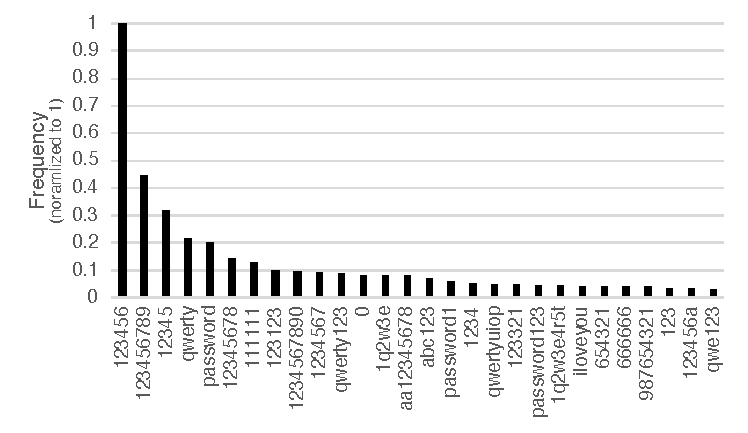
\includegraphics[width=\textwidth]{figs/password-dist.pdf}
  \caption{The most common passwords, according to
  NordPass (\url{https://nordpass.com/most-common-passwords-list/}),
  sorted by their frequency descending.
A small number of common passwords dominate.}
\end{figure}

Ideally, we would want all passwords to be equally as likely,
from the adversary's perspective.
(These would be ``high-entropy'' passwords.)
If a system generated a truly random password for each user,
each password would be indeed equally likely.
But then it becomes very difficult for a user to remember their 
password, much less many random passwords for many different services.

Typically, people have to remember their passwords,
so we let them pick their own passwords.
When they do,
it turns out that many people are likely to choose
the same password.

\marginnote[-2in]{
  \begin{tabular}{cc}
    Rank & Password \\
1 & \ttt{123456}\\
2 & \ttt{123456789}\\
    3 & 12345\\
    4 & qwerty\\
    5& password\\
    6& 12345678\\
    7& 111111\\
    8& 123123\\
    9& 1234567890\\
    10& 1234567\\
    11& qwerty123\\
    12& 000000\\
    13& 1q2w3e\\
    14& aa12345678\\
    15& abc123\\
    16& password1\\
    17& 1234\\
    18& qwertyuiop\\
    19& 123321\\
    20& password123
  \end{tabular}
  \medskip
  \captionof{table}{The most popular passwords in 2021, according to 
  NordPass, \url{https://nordpass.com/most-common-passwords-list/}.}
}

How do we convince humans to choose hard-to-guess passwords? 

\begin{itemize}
  \item \emph{Require longer passwords?} If someone tries to use 
    \ttt{abc123} as a password but it's not long
    enough, they might use \ttt{abc123456}---but
    this doesn't really add much uncertainty.
    There are standard ways to lengthen passwords,
    and a clever attacker will try these first.
  \item \emph{Prohibit using common English words in passwords?}
    It's not clear that this is a good idea.
    Five randomly chosen words from the dictionary will
    form a strong password, and prohibiting English words
    in passwords may make passwords much more difficult to remember.
      
  \item \emph{Force password changes?}
    This makes it harder for users to remember their password, and
    may actually cause users to choose easier-to-guess passwords
    (since these may be easier to remember).
    Forcing a password change may be more effective if the system has
    suffered a breach and the users' passwords have leaked out.

  \item \emph{Generate password for the user?} This is the only way
    to be guaranteed a strong password. But then the user is stuck
    having to memorize a random string.
    Few systems take this approach, mostly because it is so inconvenient
    for the system's users.

\end{itemize}

So, in spite of our best efforts, users will likely choose
easy-to-guess passwords.
What can we do about this?

\subsection{Dealing with poor passwords}
A typical password might be sampled from a distribution with roughly
20 bits of 
entropy---if an adversary is able to make $2^{20}$ guesses
at the password, they can expect to guess the password correctly.
One can computer easily make $2^{20}$
authentication requests to another in a few
minutes.
Therefore, when using passwords as an authentication
mechanism, an authentication system must \emph{always} 
somehow limit the number of password guesses.

For example, some phones allow 10 guesses at the screen-lock PIN 
before the device resets itself.
Limiting the number of guesses effectively prevents a \emph{single}
account from being compromised---provided that the password is not
too too weak.
One downside is guess limits create the possibility for denial-of-service
attacks: an attacker can potentially make 10 guesses at your password and lock
you out of your phone or online-banking account.

In addition, in many physical computer systems have multiple authorized 
users, each with their own password.
If the guess limit is enforced only on a per-user basis, then an attacker
can often compromise \emph{some} account on the machine if it is allowed
10 guesses at \emph{every} user's password.
Preventing these types of attacks requires some additional measures: websites
that use password authentication rate-limit guesses by IP, or use CAPTCHAs, etc.

\subsection{Storing Passwords on a Server}


Since, as we have seen, passwords are easy to guess, avoiding 
password-based authentication entirely is the safest option where
possible.

When a system must use passwords for authentication, the safest
way to store them (e.g., on a server) is using a
\emph{salted cryptographic password-hashing function}.
The goal is to make it as difficult as possible for an attacker
to recover the plaintext passwords, given the hashed values stored on the server.

To describe how this works: when a user creates an account with password pw,
the server chooses a random 128-bit string, called a \emph{salt},
and the server stores the salt and the hash value
$h=H(\text{salt}\|\text{pw})$, where $H$ is a special password-hashing function.

The server then stores a table that looks like this:

\medskip
\begin{tabular}{c|c|c}
  user & salt & $H(\text{salt}\|\text{pw})$ \\
	\hline
	alice & $r_a$ & $h_a$ \\
	bob & $r_b$ & $h_b$ \\
\end{tabular}
\medskip

Later on, when the user sends a password $\text{pw}'$ to the server to authenticate, 
the server can use the salt and hash function to compute a value $h' = H(\text{salt}\|\text{pw}')$.
If this hash value $h'$ matches the server's stored value $h$ for this user,
the server accepts the password.

To explain the rationale for this design:
\begin{itemize}
  \item The password-hashing function $H$ is designed to be relatively expensive
        to compute---possibly using a large amount of RAM and taking a second or 
        more of computation.
        This makes it more difficult for an attacker to brute-force invert the
        hash value, since each guess at the password requires a second of computation
        (instead of the microseconds required to compute a standard hash function,
        such as SHA256).
  \item The use of a per-user random salt ensures that guesses at one user's password
    are useless in inverting another user's password hash.\marginnote{A \emph{rainbow table}
    is a common data structure that an attacker can use to invert unsalted password hashes.
    A rainbow table is essentially a compressed table $(\texttt{passwd}, H(\texttt{passwd}))$
    pairs, where $H$ is a common hash function, and $\texttt{passwd}$ ranges over a 
    large set of common passwords.

    An attacker can download rainbow tables for common cryptographic hash
    functions, such as MD5 or SHA1, from the web.
    If the password hash is salted with a 128-bit
    salt, it will be infeasible to produce a table that covers
    any reasonably large fraction of the $(\texttt{salt}\|\texttt{passwd})$ pairs.
}
        Salting also defeats \emph{precomputation attacks}, in which an attacker
        precomputes the hashes of many common passwords to speed up this hash-inversion
        step later on.
\end{itemize}


\subsection{Storing Passwords on a Client: Password Manager}
When using passwords to authenticate to a website, 
a user can install a password manager on their
computer that will generate random passwords for them.
Since the user doesn't need to remember these passwords,
they can be sampled truly at random from a high-entropy distribution.
Once the user logs into their computer, they can
then access their randomly generated passwords and
use them to log in to their websites. 

Internally, the password-manager software maintains a table of 
servers and the corresponding passwords:

\medskip
\begin{tabular}{c|c|c}
  server & user & pw \\ \hline
  \ttt{amazon.com} & \ttt{alice} & \ttt{3xyt42...} \\
  \ttt{mit.edu} & \ttt{alice4} & \ttt{a21\$z...} \\
\end{tabular}
\medskip

But password-based authentication, even with a strong password,
still requires sending passwords over the network.
If an adversary can watch our network or can compromise the authentication
server, they can see our password.
Transport-later security, which we will discuss later on, can
protect against network eavesdroppers, but a better solution is to
authenticate without ever sending the password over the network.
That is the topic of the next section.

\section{Authentication over the Network}
We have so far been talking about a human manually
authenticating to a device (ATM, phone, laptop, etc.)
by physically entering a PIN or password into the device.
But we often log in to some server on the network---Facebook,
Gmail, MIT, and so on. 
In this scenario, we can get much more creative
with the authentication mechanism we use and the
security properties we can demand.


\subsection{Challenge-Response Protocols}
We now assume that our computer has some key~$k$
(e.g., a random 128-bit string), 
and the server also holds the same key~$k$. 
Then a challenge-response protocol proceeds as follows:

\todo{use the crypto latex library to make this nice}

\begin{enumerate}
	\item The server chooses a long random string~$r$, which we often call a \textit{nonce} and sends it to the authenticating client.
  \item The client computes an authentication ``tag'' $t \gets \MAC(k, r)$, where $\MAC(\cdot, r)$ is hard to compute without knowing $k$.
    (The function $\MAC$ here is a Message Authentication Code, which we will talk more specifically about
        in \cref{lec:mac}.)
        The sends the MAC tag $t$ to the server.
  \item The server receives a tag $t'$ from the client and ensures that $t' = \MAC(k,r)$.
        If so, the server considers the authentication successful.
\end{enumerate}

\marginnote{An \textbf{unsafe} way for the client to simultaneously authenticate to the 
server and send a request would be for the client to compute the MAC tag $t \gets \MAC(k,r)$
and then send $(t, \mathsf{req})$ to the server.
A network attacker could modify the client's request to $(t, \mathsf{req'})$ en
route to the server without the server being able to detect this attack.}
In practice, the client often wants to simultaneously authenticate to the server
and send a request $\mathsf{req}$, such as $\mathsf{req} = \ttt{rm file.txt}$.
To accomplish this, the client can compute the MAC tag $t$ as
$t_{\mathsf{req}} \gets \MAC(k, r \| \mathsf{req})$.,
Then the client sends the pair $(t_{\mathsf{req}}, \mathsf{req})$ to the server.
In this way, the server can simultaneously authenticate the client
and be sure that the request $\mathsf{req}$ came from the client.

\section{Two-Factor Authentication}
As we have already seen, passwords are a weak authentication
mechanism: humans are bad at choosing strong passwords and 
attackers have become good at stealing password databases
and recovering many users' passwords at once.

A common technique to harden password-based authentication systems
is to combine passwords with a second method of 
authentication---one with a different failure mode. 
Common authentication schemes are:

\begin{itemize}
	\item Something you know: password, PIN, etc
	\item Something you have: USB key, phone, etc
	\item Something you are: biometrics (fingerprint, face ID)...
\end{itemize}

\subsection{Time-based One-Time Passwords (TOTP)}
In this scenario, the server requests a code along
with the password. The user has a device, such as 
a phone, that shares a secret key $k$ (e.g., a random 128-bit string) 
with the server.
Both parties agree on a protocol by which to
generate this code---something like $\MAC(k, \texttt{gettimeofday() / 30})$.
The phone can generate the code, display it to the user, and the server
can then verify the code by recomputing it.

\textbf{A common attack.}\marginnote{A \emph{phishing} attack is one
in which an attacker tricks a user into giving away their Gmail password,
for example, by creating a website that looks, for example, like the \ttt{gmail.com}
login page.}
Time-based one-time passwords are also an imperfect authentication mechanism.
For example, an attacker can simply ask the user to give her the one-time code by pretend to be tech support, 
or the user's employer, or a customer-service representative.
This is essentially a phishing attack.
The code is then good for 30 seconds, so the attacker can then
just enter the code into the website on their end.
Similar attacks would include setting up a fake
website that looks like the real one, etc.
One benefit of TOTP codes (unlike passwords) is that the attacker
must use a stolen TOTP code within $\approx$30 seconds of stealing
it, which requires a much more sophisticated attack.

\subsection{Avoiding phishing: U2F (simplified)}
To prevent phishing attacks entirely, we can use a more complex authentication protocol.
If we include the name of the server that the user is trying to log in to in the request that we sent to the device,
the code will be bound to a particular website.
For example, the code might look something like $\MAC(k, r\|\ttt{amazon.com})$.
U2F key fobs use a protocol along these lines for authentication.
If the attacker sets up \ttt{amason.com} and gets the user to visit it,
the U2F device will only generate a code that is good for \ttt{amason.com}
and not the real \ttt{amazon.com}. 
	
\section{Biometrics}
Biometrics are physical features like your fingerprints, your face, etc.
They are very convenient to use for authentication, since you will not forget them and cannot easily lose them.
Biometrics most useful when authenticating in person to a device, such as for phone unlock, or
to grant a person access to a secure vault.
In these settings, the device performing the authentication has a ``trusted input path''
that can provide some assurance that a real human who owns that biometric is on the other end.
Biometrics are not so useful for authenticating over a network because the network typically
does not provide a trusted input path (i.e., does not provide any assurance that the biometric
readings are coming from a real human), and the biometric data itself is not particularly secret.
In particular, if we used biometrics for network authentication,
an adversary who knows what your fingerprints looks like could log in to your account.
(Since biometrics are essentially impossible to change, this is a major drawback.)

\chapter{Collision Resistance and File Authentication}

In the last chapter, we focused on authenticating people---ensuring that
a person (or a request on behalf of that person) is likely who they claim to be.
In this chapter, we will focus on authenticating
files, code, and other data.
When we say that we want to authenticate a file,
we mean that we want to verify that the file's
contents are exactly as they were when we or
someone we trust last viewed them.
The key new tool we use to do so is a \textit{collision-resistant hash function}. 

\section{Intuition: Collision resistance}
For our purposes, a hash function $H$ 
maps a bitstring of any length onto a fixed-size space of outputs,
so the type signature is $H: \bin^* \rightarrow \bin^{\lambda}$.

In order for a hash function to be \textit{collision-resistant}, we want it to be the case that for any input, the generated output should be \textquote{unique.} Of course, it cannot really be unique---we are mapping infinitely many inputs onto finitely many outputs---but we want it to be \textit{computationally infeasible} to find a 
pair of distinct inputs that have the same hash values (a ``collision'').

\begin{framed}
\noindent
\textbf{Security goal:} A hash function $H$ is \emph{collision resistant} if
it is \textquote{computationally infeasible} to find two distinct strings
$x$ and $x'$ such that $H(x) = H(x')$.
\end{framed}

Given a long message $m$, it's hash $H(m)$ under a collision-resistant
hash function is like a short ``fingerprint'' of the message---the
hash essentially uniquely identifies the message $m$.
For that reason, collision-resistant hash functions let you authenticate 
a long message $m$ by authenticating the  short fixed-length string $H(m)$.
We often call the hash value $H(m)$ a \emph{digest}.

\subsection{Applications}
\subsubsection{Secure File Mirroring}
Often a user wants to download large files (e.g., software updates) from a far-away server.
To speed up this process, a company or Internet-service provider may set up local \emph{mirrors}
of the remote files.
Users can then download the files from the nearby mirror instead of the far-away server.
However, without additional security measures, the mirror may 
server users a different file than the one the mirror fetched from the origin server.
If the mirror is malicious, it can, for example, trick the user into installing
a backdoored software update.
(We saw an attack based on mirrors in~\cref{sec:intro:xcode}.)

To protect against a malicious mirror, we can add some authentication on the file that the mirror hosts.
Say that the origin server publishes a large software update~$f$.
The origin server will send the file $f$ to its mirrors and the origin
server itself will serve the hash digest $d\gets H(f)$ to anyone who asks for it.
A user who wants to fetch the update can download $d$ from the origin server directly---this
will be fast since the digest is tiny.
Then, the client can fetch the update itself from a (potentially untrustworthy) mirror.
When the client receives a file $\hat f$ from the mirror, it can check that $d = H(\hat f)$
to ensure that $\hat f$ is the true software update.
If $H$ is collision resistant, then if the hash value $H(\hat f)$ matches the origin server's digest $d$,
the files are almost certainly identical.

\subsubsection{Subresource Integrity}
If a program fetches a file from some content
delivery network, it can store the hash of that
file locally and use it to verify that the
contents of the file did not change since the
application was developed.

\subsubsection{Outsourced File Storage}
If you want to store your files on a cloud
provider, you want to be sure that the cloud
provider does not maliciously modify the files
without you noticing. To make sure of this, you
can store $H(\text{files})$ locally, which takes
very little storage space. Then, when you
redownload your files locally, you can recompute
the hash to verify that they were not tampered
with.

\section{Defining collision resistance (slightly more formally)}
An adversary's goal in breaking a collision
resistant hash function is to find a collision---a
pair of values $m_0, m_1 \in \zo^*$ such that
$m_0 \neq m_1$ and $H(m_0) = H(m_1)$.

\begin{definition}[Collision Resistance]\label{def:crhf}
	A function $H: \bin^* \rightarrow \bin^{\lambda}$ is collision-resistant 
  if for all \textquote{efficient} adversaries $\calA$, we have that:
  \[ \Pr[H(m_0) = H(m_1), m_0 \neq m_1: (m_0, m_1) \leftarrow \calA()] \leq \text{``negligible''} \]
\end{definition}

In words, this means that the probability of finding a collision is so small that no efficient adversary could hope to do it.

There are two ways of thinking about the terms ``efficient'' and ``negligible'' that 
we use in this definition---one mindset we use in practice and the other mindset we use in theory.

\begin{itemize}
	\item In theory$\ldots$
		\begin{itemize}
      \item All of our cryptographic constructions are parameterized by an integer $\lambda \in \{1, 2, 3, \dots\}$
            that we call the \textit{security parameter}.
            So instead of a single collision-resistant hash function $H$, we have a family of functions
            $\{ H_1, H_2, H_3, \dots \}$, where the function $H_\lambda$ has $\lambda$-bit output. 
			\item An \textquote{efficient} algorithm is a randomized algorithm that runs in time polynomial in $\lambda$.
			\item A \textquote{negligible} function is one that grows slower than the inverse of every polynomial---a function that is $O(\frac{1}{\lambda^c})$
            for all constants $c \in \mathbb{N}$.  
		\end{itemize}
	\item In practice$\ldots$
		\begin{itemize}
			\item We use a fixed hash function $H$ with a fixed-length output,
        which might be as 256 or 512 bits.
			\item An \textquote{efficient} adversary is one that runs in time $\leq 2^{128}$.
			\item A \textquote{negligible} probability is some very small constant, like one smaller than $2^{-128}$.
		\end{itemize}
\end{itemize}

\subsection{Understanding which attacks are feasible}

Typically, we think of an attack that runs in more than $2^{128}$ time
as infeasible and an event that happens with probability less than $2^{-128}$
is one that will never happen.
These seemingly magic constants come from empirical considerations:

\begin{table}[htpb]
	\centering
	%\caption{Big numbers in terms of hashes}
	%\label{tab:exp-work}

	\begin{tabular}{rl}
		$2^{30}$ & operations/second on a laptop \\
		$2^{58}$ & ops/sec on Fugaku supercomputer \\
		$2^{68}$ & hashes/second on the Bitcoin network (as of Fall 2022) \\
    $2^{92}$ & hashes/yr on the Bitcoin network\\
		$2^{114}$ & hashes required to use enough energy to boil the ocean \\
		$2^{140}$ & hashes required to use one year of the sun's energy \\
	\end{tabular}
\end{table}

See Lenstra, Kleinjung, and Thom{\'e} for an entertaining
discussion of these constants.\autocite{lenstra:universal}

\begin{table}[htpb]
	\centering
  %\caption[Exponents as probabilities][3em]{Exponents as probabilities}
	%\label{tab:exp-probability}

	\begin{tabular}{rl}
		$2^{-1}$ & fair coin lands heads \\
    $2^{-13}$ & \parbox{3.5in}{probability that a randomly sampled\\[-3pt] MIT grad is a Nobel Prize winner}\\
    $2^{-19}$ & probability of being struck by lightning next year\\
		$2^{-28}$ & probability of winning the Mega Millions jackpot\\
		$2^{-128}$ & will essentially never happen \\
	\end{tabular}
\end{table}



\marginnote{For most cryptosystems, there is a tradeoff between the
attacker's running time and success probability.
For example, an attacker running in time $T$ can find a collision in
a hash function with $n$-bit output with probability $T^2/2^n$.
So, as the attack runs for more time, it has a better chance of
finding a collision.
}
The takeaway is that if an attacker finds a collision with probability
$2^{-128}$, we can be extremely sure that a collision will never occur.

\section{Constructing a collision-resistant hash function}
The current standard for fast collision-resistant
hashing is SHA256 (a.k.a. SHA2), which was designed by the NSA in 2001.
The SHA2 hash functions are designed using the following common
two-step approach:

\marginnote{
We can also build collision-resistant hash functions
that are secure under \textquote{nice} cryptographic assumptions,
such as the assumption that factoring large numbers is hard.
Unfortunately, hash functions based on
these nice assumptions tend to be very slow and, as a result, 
are almost never used in practice.
}

\begin{enumerate}
  \item Build a small collision-resistant hash
    function on a fixed-size domain $H_{small}: \bin^{2\lambda} \rightarrow \bin^\lambda$.
    This step is, to some degree, \textquote{more art than science}.
    The standard practice is to design a hash function that
    defeats all known collision-finding attacks.
    If no known attack works well, we declare the
    candidate function to be collision resistant.

	\item Use $H_{\text{small}}$ to construct $H: \bin^* \rightarrow \bin^\lambda$.
    This can be done very cleanly using the \textquote{Merkle-Damg\aa{}rd} approach described
    below.
    This step requires no additional assumptions:
    we can prove unconditionally that if $H_{\text{small}}$ is
    collision resistant, then $H$ is as well.
\end{enumerate}

\marginnote{Another way to build collision-resistant hash functions
is to use the so-called ``sponge'' construction.
It is similar to the approach described here in that we start
with a small primitive, which we assume secure in some sense, 
and then we use the small primitive to build a hash function
on a large domain.}

\subsection{Merkle-Damg\aa{}rd}
The Merkle-Damg\aa{}rd construction gives a way to construct
a collision-resistant hash function for all bitstrings (i.e., $\zo^*$)
from a collision resistant hash function that maps $2\lambda$-bit strings
down to $\lambda$-bit strings, sketched out in \Cref{fig:merkle-damgard}.

\begin{figure}[htpb]
  \centering
  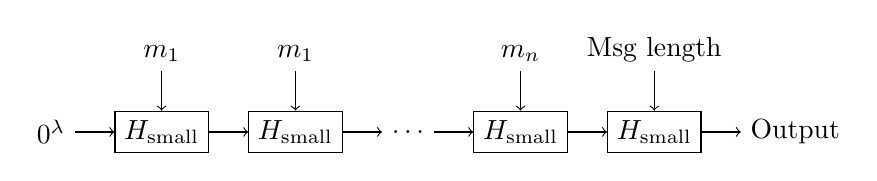
\begin{tikzpicture}
    \node (iv) {$0^\lambda$};
    \node [right=.5cm of iv] (H1) [draw] {$H_\textrm{small}$};
    \draw [->] (iv) edge (H1);
    \node [above=.5cm of H1] (m1) {$m_1$};
    \draw [->] (m1) edge (H1);
    \node [right=.5cm of H1] (H2) [draw] {$H_\textrm{small}$};
    \draw [->] (H1) edge (H2);
    \node [above=.5cm of H2] (m2) {$m_1$};
    \draw [->] (m2) edge (H2);
    \node [right=.5cm of H2] (Hdot) {$\ldots$};
    \draw [->] (H2) edge (Hdot);
    \node [right=.5cm of Hdot] (Hn) [draw] {$H_\textrm{small}$};
    \draw [->] (Hdot) edge (Hn);
    \node [above=.5cm of Hn] (mn) {$m_n$};
    \draw [->] (mn) edge (Hn);
    \node [right=.5cm of Hn] (Hfinal) [draw] {$H_\textrm{small}$};
    \draw [->] (Hn) edge (Hfinal);
    \node [above=.5cm of Hfinal] (len) {Msg length};
    \draw [->] (len) edge (Hfinal);
    \node [right=.5cm of Hfinal] (out) {Output};
    \draw [->] (Hfinal) edge (out);
  \end{tikzpicture}
  \caption{Sketch of the Merkle-Damg\aa{}rd construction for a
    collision-resistant hash function.}
  \label{fig:merkle-damgard}
\end{figure}


The Merkle-Damg\aa{}rd construction first splits the
message into $\lambda$-sized blocks $[m_1, \ldots, m_n]$ and successively hashes them together.
In the following pseudocode,
the function $\mathsf{ToBlock}$ converts an integer, representing the length of the input message
in blocks, into a $\lambda$-bit string.
Then the Merkle-Damg\aa{}rd construction is:
\begin{figure}
\begin{framed}
\noindent
  $H(m_1, \dots, m_n)$: \qquad \text{// Merkle-Damg\aa{}rd construction}
\begin{itemize}[noitemsep]
  \item Let $b \gets 0^\lambda$.
  \item For $i = 1, \dots, n$:
   \begin{itemize}
     \item Let $b \gets H_\text{small}(b, m_i)$.
   \end{itemize}
 \item Let $b \gets H_\text{small}(b, \mathsf{ToBlock}(n))$.
 \item Output $b$.
\end{itemize}
\end{framed}
\caption{The Merkle-Damg\aa{}rd construction of a large-domain
collision-resistant hash function $H$ from a small-domain
collision-resistant hash function $H_\text{small}$.}
  \label{fig:md}
\end{figure}
(Here, we are assuming that the message is at most 
$\lambda 2^{\lambda}$ bits long.)
\marginnote{In practice, standard hash functions have limits on the
length of the messages that they can hash. For example, SHA256 can
hash messages of length up to $2^{64}-1$ bits.}

We won't prove it here, but we can use the fact that $H_{small}$ is collision-resistant to prove that $H$ must also be collision-resistant. The basic idea of the proof is to show that given a collision in $H$, we can easily compute a collision in $H_{\text{small}}$. 

\paragraph{Note:} In 
the Merkle-Damg\aa{}rd construction of \cref{fig:md},
we initialize the variable $b$ to the all-zeros string.
The construction is collision-resistant if we omit the all-zeros
string and start by setting $b \gets m_1$ and then continue by hashing $m_2, m_3, \dots$.
The construction is \emph{not} collision resistant if we omit the length block
$\mathsf{ToBlock}(n)$ that we hash in at the end.


\subsection{The Birthday Paradox}
\marginnote{If you sample $2^{\lambda/2}$ random $10\lambda$-bit strings and hash them
with a hash function that has $\lambda$-bit outputs, you will find a collision 
among these inputs with constant probability.}
An important thing to understand when dealing with hash functions is the ``Birthday Paradox,'' 
which states that given a hash function with $\lambda$-bit output, you can 
always find a collision in time $O(\sqrt{2^\lambda}) = O(2^{\lambda/2})$.
So, if you want to force an attacker to use at least $2^{128}$ to find a collision,
you must use a hash function with at least 256 bits of output.

\subsection{Domain Separation}
In many applications, we have a one-input CRHF (such as SHA256) $H: \bin^* \rightarrow \bin^{256}$ 
and we need to construct a two-input CRHF $H_2(x, y)$. 

\paragraph{Bad idea.} An obvious solution to construct the two-input hash function $H_2$ 
is to concatenate the two values, so that $H_2(x, y) = H(x || y)$.
However, this construction allows two different pairs of messages to hash to the same value:
\[H_2(\text{"key", "value"}) = H_2(\text{"ke", "yvalue"}).\]
Both Amazon and Flickr had a bug arising from
this---they concatenated all parameters before
hashing, and had parameters such that two
different intents had the same concatenation.\autocite{flickr}

\subsection{Length-Extension}
Recall the concept of Message Authentication Codes
(MAC) from the last lecture---a code that can be
sent along with a message to verify that the message was not changed.
(We will see the formal definition in \cref{lec:mac}.)

\paragraph{Bad idea.}
Poorly designed software uses $\MAC(k, m) = H(k \| m)$ as a very simple construction of a MAC.
However, this construction has an easy attack---given $\MAC(k, m)$, it is easy to compute $\MAC(k, m\|m')$ 
without knowing the key $k$ if $H$ is a hash function built with the Merkle-Damg\aa{}rd construction.
To do this, the attacker hashes the output of $\MAC(k, m)$ with two more blocks---a new 
message $m''$ and another length block. Now, we
have computed $\MAC(k, m\|m')$ where $m'$ is the
original length block plus some custom message
without knowing the key~$k$. 

This problem here is that we were using a hash
function that was \emph{only} guaranteed to be
collision resistant, but we assumed that it had other
properties (such as that it is guaranteed to be
difficult to compute the hash of an extension of
the original message).  \Cref{fig:merkle-damgard-extension}
sketches out the length-extension attack on the Merkle-Damg\aa{}rd
construction from \Cref{fig:merkle-damgard}.

\begin{figure}[htpb]
  \centering
  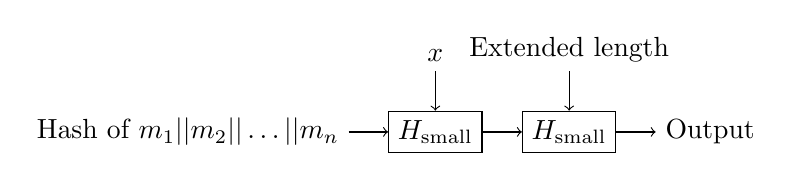
\begin{tikzpicture}
    \node (start) {Hash of $m_1 || m_2 || \ldots || m_n$};
    \node [right=.5cm of start] (H1) [draw] {$H_\textrm{small}$};
    \draw [->] (start) edge (H1);
    \node [above=.5cm of H1] (x) {$x$};
    \draw [->] (x) edge (H1);
    \node [right=.5cm of H1] (Hfinal) [draw] {$H_\textrm{small}$};
    \draw [->] (H1) edge (Hfinal);
    \node [above=.5cm of Hfinal] (len) {Extended length};
    \draw [->] (len) edge (Hfinal);
    \node [right=.5cm of Hfinal] (out) {Output};
    \draw [->] (Hfinal) edge (out);
  \end{tikzpicture}
  \caption{Sketch of the extension attack on the Merkle-Damg\aa{}rd
    construction, starting with a hash of $m_1 || m_2 || \ldots || m_n$
    to compute the hash of $m_1 || m_2 || \ldots || m_n || \textsf{ToBlock}(n) || x$.}
  \label{fig:merkle-damgard-extension}
\end{figure}


\section{Applications: Merkle Trees}
In many settings, an origin server has $N$ files (e.g., Android app binaries)
and wants to serve these files from potentially untrustworthy mirror servers
(e.g., Akamai servers) distributed around the globe.

To do this, the origin server can put the $N$ files at the leaves of a
binary tree.
Then the server hashes together pairs of files, then hashes each pair of
hashes and so on until it eventually ends up with
a single root hash $h$.
The client fetches the root hash $h$ from the origin
server directly.

Later on, the client can download any one of the $N$
files from the untrustworthy mirror server.
The mirror can produce the file, along
with $O(\log N)$ hashes---the sibling
nodes of each node on every path from the file's
leaf to the root.
The client can use the root hash $h$ it got from
the origin server, along with the additional hashes
from the mirror server, to be convinced that the mirrored
file it downloaded was authentic.

\todo{Add diagram from lecture.}


\chapter{Message Authentication Codes}

\label{lec:mac}

So far, we have talked about authenticating \emph{people} and authenticating \emph{files}. In this section, we will discuss authenticating \emph{communication}. If we have two parties that are communicating over the network, we want some way to guarantee to each party that the message they received really came from the other party and was not tampered with along the way.

At a first glance, this seems impossible. If there is some eavesdropper Eve in between the two parties, they can just replace the message with one of their own choosing and the other party will have no idea. To make this possible, we need to relax the scenario a bit and add an assumption---that the two parties share some secret key $k$. 

With this shared key $k$ between the two parties, our goal will be to add some \textquote{tag} onto the message that validates its authenticity. Necessarily, this tag will be a function of this shared key $k$. If this were not the case, the eavesdropper would be able to compute a valid tag herself---the secret $k$ is the only information in this scenario that Eve does not know.

% figure out how to use cryptocode and make a diagram like

%    k              k 
% client -------> server
%         m, tag
%\procedureblock

\section{Defining message authentication codes}

\paragraph{Syntax.}
A message authentication code (MAC) 
over key space $\mathcal{K}$, 
message space $\mathcal{M}$ , and tag space $\calT$
is an efficient algorithm 
$\MAC \colon \calK \times \calM \to \calT$.
In order for a MAC to be useful, it must be \emph{secure},
in the following sense.
We first give the definition and then explain why it is a useful
one:

\begin{definition}[MAC Security: Existentially unforgeability against adaptive chosen message attacks]\label{def:mac-sec}
A MAC $\MAC$ over key space $\calK$ and message space $\mathcal{M}$ is secure 
(existentially unforgeable against adaptive chosen
message attacks) if any poly-time adversary
$\mathcal{A}$\marginnote{In practice,
\textquote{a poly-time adversary} means
\textquote{any real-life adversary}. But we need
to place some mathematical bound on real-life to
make the proofs work out.} wins the following
game with at most negligible probability:
  \begin{itemize}[noitemsep]
    \item The challenger samples a MAC key $k \getsr \calK$.
    \item For $i = 1, 2, \dots$ (polynomially many times)
      \begin{itemize}
        \item The adversary sends any message $m_i \in \calM$ 
              to the challenger 
        \item The challenger responds with $\mathsf{MAC}(k, m_i)$. 
      \end{itemize}
    \item The adversary sends the challenger a message-tag pair $(m^*, t^*)$.
    \item The adversary wins the game if $\mathsf{MAC}(k, m^*) = t^*$ and $m^* \notin \set{m_1, m_2, \ldots, m_n}$.
  \end{itemize}
  \marginnote{A subtlety of this definition is that, even if the MAC scheme is
  secure under this definition, it is possible for an adversary, given 
  a valid message-tag pair $(m,t)$ to produce a second valid message-tag pair
  $(m,t')$ on the same message without knowing the secret key.
  }

	% TODO: finish this diagram
	%\procedureblock{MAC Security}{
	%	$\mathcal{A}$ \> \> \textbf{Ch} \\
	%}
\end{definition}

\subsection{Intuition for the security definition}
To formulate our security notion, we need to define
the adversary's goal and the adversary's power.

The adversary's goal in this definition is 
to compute a valid MAC of \emph{any} message $m\in \mathcal{M}$
of its choice.
It's not entirely obvious why we care about the adversary producing 
a valid MAC on \textit{any} message: ``If the
adversary MACs a message that is jibberish, they
are unlikely to be able to do any harm with it,''
you might think. 
But there will certainly be applications
that authenticate messages that violate whatever
definition of \textquote{non-jibberish} we define.
So allowing the adversary to forge a MAC tag on any 
message makes the definition as broadly applicable as possible.

\marginnote{This has some interesting implications---importantly, the adversary can store these messages along with their MAC and replay them later.}
As far as the adversary's power goes: we, as usual in cryptography,
restrict the adversary to be efficient (i.e., to run in polynomial time).
But in the MAC security game we also allow the adversary to obtain
MAC tags on messages of its choice.
This captures the reality that in many systems, an adversary can trick
an honest system into MACing adversarial messages.
For example, if an email-backup system MACs every email that a
user receives, an adversary may be able to obtain MAC tags on messages
of its choice by sending emails to the backup system.


\subsection{MACs require pseudorandomness}
The fact that it is even possible to construct a MAC seems a bit surprising---in effect, for a MAC to satisfy the definition, the tag has to effectively be random. But the only \textquote{randomness} that we have is the key $k$---to generate tags for arbitrarily many messages, we need much more randomness than one key's worth. This seems impossible.
How can we generate a large number of random-looking tags from only a single
short random key?

We get ourselves out of this conundrum by observing that the adversary
must be an \emph{efficient} algorithm.
So while we cannot generate a large number of truly random bits from a
short key, we can---under appropriate and reasonable
cryptographic assumptions---generate a large number of bits that \emph{look}
truly random from the perspective of any efficient algorithm.
We call these bits \emph{pseudorandom}.

This surprising and powerful idea leads us to our next cryptographic primitive\ldots

\section{Pseudorandom Functions}

A pseudorandom function is defined over a keyspace $\calK$,
and input spacei $\calX$ and output space $\calY$.
To be useful a pseudorandom function must satisfy the following
security definition:

\begin{definition}[Pseudorandom Function, PRF]\label{defn:prf}
A function $F: \mathcal{K} \cross \calX \rightarrow \calY$ is a pseudorandom
function if all efficient algorithms $\mathcal{A}$ win
the following game with probability $\tfrac{1}{2} + \text{\textquote{negligible}}$: 

  \begin{itemize}[noitemsep]
    \item The challenger samples a random bit $b \gets \zo$ and a key $k \getsr \calK$.
    \item If $b = 0$, the challenger sets $f(\cdot) \deq F(k, \cdot)$.
    \item If $b = 1$, the challenger sets $f(\cdot) \getsr \Funs[\calX, \calY]$.
      \marginnote{Here, $\Funs$ is the set of all functions from $\calX$ to $\calY$.}
    \item Then for $i = 1, 2, \dots$ (polynomially many times):
      \begin{itemize}
        \item The adversary sends the challenger a values $x_i \in \calX$.
        \item The challenger responds with $y_i \gets f(x_i) \in \calY$.
      \end{itemize}
    \item The adversary outputs a guess $\hat{b}$ at the bit $b$.
    \item The adversary wins if $b = \hat{b}$.
  \end{itemize}
First, the challenger will sample a random $b \leftarrow \bin$ and a key $k \leftarrow \mathcal{K}$. 
\end{definition}

The adversary can trivially win this game with
probability $\tfrac{1}{2}$ by just guessing the
bit $b$ at random.
This definition asserts that
no efficient adversary can do much better than that.

If we have such a pseudorandom function $F$, we
could easily construct a MAC---we can just use the
message as the input to the pseudorandom function
along with the key: $\MAC(k, m) \deq F(k, m)$.


\subsection{Constructing pseudorandom functions from one-wayness}

It is not at all obvious that pseudorandom functions should exist
at all! They seem like a very magical primitive indeed.

One surprising fact is that if there exists \emph{any} function that
is ``hard to invert,`` in a sense we will define, then pseudorandom
functions exist.
For example, if you believe that factoring large numbers is difficult
(as many people do), then pseudorandom functions exist.

In particular the following definition captures the notion of a
function that is hard to invert:
\begin{definition}[One-Way Function]\label{def:owf}
A function $f \colon \calX \to \calY$ is a \emph{one-way function} if
for all efficient adversaries $\calA$, 
\[ \Pr[f(\calA(f(x))) = f(x) \colon x \getsr \calX ] \leq \text{``negligible''}.\]
\end{definition}

Having defined one-way functions, we now have the following surprising and
non-obvious result:\marginnote{Notice that if
$\classP = \classNP$, one-way functions do not exist,
and therefore psuedorandom functions do not exist.
}
\begin{theorem}
Psueodorandom functions exist if and only if one-way functions exist.
\autocite{HILL99}
\end{theorem}

In practice, we assume that:
\begin{itemize}
  \item the function $f(x) \deq \text{SHA256}(x)$ is a one-way function
    where the domain is the set of 256-bit strings,
  \item the function $f(x) \deq \text{AES}(x, 0^{128})$ is a one-way function,
    where the domain is the set of 128-bit strings, and
  \item the function $f(x) \deq 2^x \bmod p$ is a one-way function
    on domain $\{1, \dots, p\}$, for a sufficiently large prime $p$.
\end{itemize}

\subsection{Pseudorandom functions in practice}

In practice, we use the Advanced Encryption
Standard (AES) as a pseudorandom function.
The AES function on key length $\kappa \in \{128, 192, 256\}$
has the type signature
$\mathsf{AES}: \bin^\kappa \times \bin^{128} \rightarrow \bin^{128}$.
That is, it takes a 128-bit input and generates a 128-bit output.
\marginnote{We
don't have any mathematical proof that AES is
a pseudorandom function. However, 
it has undergone a tremendous amount of cryptanalysis and the best attacks on AES are only marginally better than the obvious brute-force attacks.}

\section{From pseudorandom functions to MACs}

\paragraph{MACs for short messages.}
Using AES as a pseudorandom function on a 128-bit domain,
we can build a MAC for 128-bit messages as described above
: $\MAC(k, m) \deq \mathsf{AES}_k(m)$. 
However, since AES takes only 128 bits as input, using AES
directly, we can only authenticate 128-bit messages. 

\paragraph{Insecure ways to construct a MAC for long messages.}
A bad way to construct a MAC for long messages from a pseudorandom 
function $F$ for 128-bit messages is
just to chop our message $m$ up into 128-bit blocks
$m = (m_1, m_2, \dots)$
and MAC each block separately.
Our tag, then, would look something like $\left(F(k,m_1), F(k,m_1)\right)$.
However, there is a problem! Given the tag $t = (t_1, t_2)$ for a message $m=(m_1, m_2)$, we can easily generate a valid tag 
$t' = (t_2, t_1)$ for a different message $m'=(m_2, m_1)$. 

\paragraph{MACs for long messages: The easy way.}
\marginnote{
Notice that we cannot use AES as the pseudorandom
function $F$ in this construction, since AES only
takes a 128-bit input.
In this case, we would need a collision-resistant
hash function $H \colon \zo^* \to \zo^{128}$,
but it is always possible to find collisions
in hash functions with 128-bit output in time $2^{64}$.
So such a MAC can never be secure against attackers running
in time $2^{64}$.
}
If we have a pseudorandom function $F$ with an input space of 256-bits,
we can construct a MAC on arbitrary-length messages using the ``hash-and-sign'' paradigm.
In particular, we use a collision-resistant hash function $H\colon \zo^* \to \zo^{256}$ 
(\cref{def:crhf}) and we define the MAC on message space $\zo^*$ as:
\[ \MAC(k,m) \deq F(k, H(m)).\]


In practice, we typically do not construct MACs in this way because
collision-resistant hash functions are typically more expensive to
compute (per bit of input) than pseudorandom functions, such as AES.

\subsection{MACs for long messages: Cipher-Block Chaining MAC}

\marginnote{
Applying the PRF to the last block using an independent random key is important.
If we do not use a new key, an adversary can mount a length-extension attack.
That is, if the adversary asks for $t = \mathsf{MAC}(k, m_1)$ and $t' = \mathsf{MAC}(k, t)$, $t'$ is also a valid key for the original message with two zero blocks attached $\mathsf{MAC}(k, m_1 \| 0 \| 0)$. The chain of AES applications becomes equivalent, since zero blocks are equivalent to skipping the XOR and adding AES applications.
}

A common and secure way to construct a MAC for long messages from a MAC for short messages
is to \emph{chain} the output of each of these calls to the pseudorandom function.
Given our chopped message $(m_1, m_2, \ldots, m_n)$, we will generate $t_1 = F(k,m_1)$ as before. When generating $t_2$, we will first XOR $t_1$ into the input: 
$t_2 = F(k, m_2 \oplus t_1)$. This continues until the end of the message, at which point have a tag $t_n$.
Finally, we apply the PRF \emph{with a different key} $k'$ to the value $t_n$ and output this tag $t \gets F(k', t_n)$. 
This construction is called CBC-MAC or CMAC. % TOOD: explanation of why we need a second key here would be useful---the diagram in lecture 9/21 was very useful to understand the same-key attack.


\begin{figure}[htpb]
	\centering
	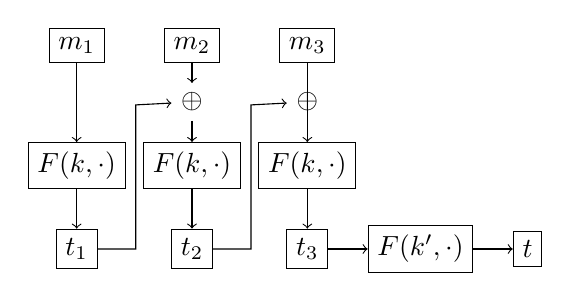
\begin{tikzpicture}
		\node (m0) [draw] {$m_1$};
    \node[below =1cm of m0] (f0) [draw] {$F(k, \cdot)$};
		\node[below =0.5cm of f0] (t0) [draw] {$t_1$};
		\draw [->] (m0) edge (f0) (f0) edge (t0);

		\node[right=0.75cm of m0] (m1) [draw] {$m_2$};
		\node[below =0.25cm of m1] (m1xt0) {$\oplus$};
		\draw [->] (t0) - ++(0.75,0) -- ++(0.75,1.83) -- (m1xt0);
    \node[below =1cm of m1] (f1) [draw] {$F(k, \cdot)$};
		\node[below =0.5cm of f1] (t1) [draw] {$t_2$};
		\draw [->] (m1) edge (m1xt0) (m1xt0) edge (f1) (f1) edge (t1);

		\node[right=0.75cm of m1] (m2) [draw] {$m_3$};
		\node[below =0.25cm of m2] (m2xt1) {$\oplus$};
		\draw [->] (t1) - ++(0.75,0) -- ++(0.75,1.83) -- (m2xt1);
    \node[below =1cm of m2] (f2) [draw] {$F(k, \cdot)$};
		\node[below =0.5cm of f2] (t2) [draw] {$t_3$};
    \node[right=0.5cm of t2] (out) [draw] {$F(k', \cdot)$};
    \node[right=0.5cm of out] (outp) [draw] {$t$};
		\draw [->] (m2) edge (f2) (f2) edge (t2);
    \draw [->] (t2) edge (out);
    \draw [->] (out) edge (outp);
	\end{tikzpicture}
  \caption{The CBC-MAC construction.}
	\label{fig:}
\end{figure}

CBC-MAC is going out of favor for two reasons:
\begin{enumerate}
  \item It is impossible to parallelize the MAC computation:
        the chaining procedure is inherently sequential so you 
        cannot speed it up, even if you have a computer with many 
        CPU cores.
  \item Computing the MAC requires one PRF invocation \emph{per block} of the message.
        There are even faster MACs that require only one PRF invocation
        \emph{per message} total, 
        plus a number of fast ``non-cryptographic'' operations
        per message block.
        These MACs can be faster than CBC-MAC on some processors.
        The GMAC construction we will see next is one example.
\end{enumerate}

% TODO: diagram

\subsection{A parallelizable MAC: Carter-Wegman MAC}\label{sec:mac:cw}

We now describe a different way to authenticate long messages.
This MAC scheme is parallelizable and also requires only one 
single PRF invocation per message authenticated (independent of
the message length).
The construction is named the Carter-Wegman MAC, after its
inventors.\autocite{CW81}
Modern encryption schemes, including AES-GCM (\cref{sec:enc:gcm})
use a Carter-Wegman-style MAC as a key ingredient.

For this construction, we will use the notation
$\Z_p$ to indicate the set of integers modulo $p$
with addition and multiplication modulo $p$.
So $x + y \in \Z_p$ means that we add $x$ and $y$
as integers and reduce the result modulo~$p$.
Typically, we will think of $p$ as a prime---of
64 bits, for example.
The construction uses a fixed a prime number $p$ as a parameter,
where $p \approx 2^n$ for security parameter $n$.\marginnote{So
in practice, we take $p \approx 2^{128}$
for 128-bit security.}

\paragraph{Universal hash function.}

Before we look at the construction of the Carter-Wegman MAC, we first
define an important building block: the notion of a \emph{universal hash
function}, or UHF for short.  A universal hash function is keyed, and
provides collision-resistance when the adversary does not know the key.
Specifically, we say that $H$ is a universal hash function if, when an
adversary chooses two messages $m$ and $m'$ where $m\neq m'$,

$$
Pr[H(k, m) = H(k, m')] \leq \text{negl.}
$$

Intuitively, a universal hash function is a weaker primitive than a
collision-resistant hash function: the adversary does not know the
precise hash function that will be applied to their messages, because
the adversary does not know what key will be used.

One simple and practical construction of a universal hash function
is based on polynomials.  Given a long message $m$, break it up into
fixed-size chunks $m_0, m_1, \ldots, m_{l-1}$.\marginnote{In practice,
these fixed-size chunks are going to be 128 or 256 bits long.}  Then,
the hash of that message is defined as:

$$
H(k, m_0 || m_1 || \ldots || m_{l-1}) = (m_0 + m_1 k + m_2 k^2 +
  \ldots + m_{l-1} k^{l-1}) \mod p
$$

We can give some intuition for why $H$ is a universal hash function
(i.e., collision-resistant for a randomly chosen key).  In order for
a pair of messages $m$ and $m'$ to collide, it must mean that
$H(k, m) = H(k, m')$, which in turn means that $H(k, m) - H(k, m') = 0$.
Expanding the definition of $H$ as a polynomial, this means that

$$
(m_0 - m'_0) + (m_1 - m'_1) k + (m_2 - m'_2) k^2 + \ldots + (m_{l-1} - m'_{l-1}) k^{l-1} = 0
$$

which is another way of saying that $k$ is a root of that degree-$l-1$
polynomial.  We know that there can be at most $l-1$ roots of a
degree-$l-1$ polynomial, but there are $p \approx 2^n$ possible choices
for $k$, so the probability that our randomly-chosen $k$ happens to be
one of those roots is $\frac{l-1}{p}$, which is negligible.

\paragraph{MAC construction.}

The MAC uses a pseudorandom function 
$F \colon \calK \times \Z_p \to \Z_p$.
\marginnote{Here, the input space of the pseudorandom 
function $F$ is the set of integers in $\{0, \dots, p-1\}$.
Given a pseudorandom function on bitstrings, it is indeed
possible to construct one that operates on numbers in 
$\Z_p$ like this by interpreting each number as a bitstring.}
The keyspace for the MAC is $\calK$, so the MAC key consists of a key for 
the pseudorandom function.
The message space for the MAC is $\calM = \Z_p^{\leq L}$,
the set of vectors of integers of $\Z_p$ elements of length
at most $L$ where $L \ll p$.
Here, assume that the message vector has length at least $1$.

One other difference is that this MAC construction is 
\emph{randomized}. So there are now two algorithms:
\begin{itemize}
  \item $\MACSign(k, m) \to t$, which takes as input a key $k$ and message $m$
        and outputs a MAC tag $t$, and 
  \item $\MACVerify(k, m, t) \to \zo$, which takes as input a key $k$,
    message $m$, tag $t$, and outputs an accept/reject bit.
\end{itemize}
The security definition here is essentially the same as for deterministic MACs,
except that we use different algorithms to generate and verify the MAC tags.

The Carter-Wegman MAC construction is then:

\medskip
\noindent
$\MACSign(k, m \in \Z^{\leq L}_p) \to t$.
\begin{itemize}[noitemsep]
  \item Compute $v \gets F(k, 0) \in \Z_p$.
  \item Parse the message into chunks as $(m_1, \dots, m_{\ell}) \gets m \in \Z_p^\ell$.
  \item Compute $M(v) \gets m_1 v + m_2 v^2 + m_3 v^3 \cdots + m_{\ell} v^{\ell} \in \Z_p$. \\
        \marginnote{Essentially we are viewing the blocks of the message 
        $m$ as coefficients of a degree-$t$
        polynomial $M(\cdot)$. We then evaluate this polynomial 
        at the secret point $v$ determined by the MAC key.}
        \hcg{Check the definition of the message polynomial $M$. Should 
        there be an additional $v^{t+1}$ monomial?}
  \item Sample a nonce $r \getsr \Z_p$.
  \item Output $t \gets \big(r, F(k, r) + M(v)\big) \in \Z^2_p$ as the MAC tag.
\end{itemize}

\medskip
\noindent
$\MACVerify(k, m, t) \to \zo$.
\begin{itemize}[noitemsep]
  \item Compute $v \gets F(k, 0) \in \Z_p$.
  \item Parse the message into chunks as $(m_1, \dots, m_{\ell}) \gets m \in \Z_p^\ell$.
  \item Compute $M(v) \gets m_1 v + m_2 v^2 + m_3 v^3 + \cdots + m_{\ell} v^{\ell}\in \Z_p$. \\
  \item Parse the tag $(r, z) \gets t \in \Z^2_p$.
  \item Output ``1'' if and only if $z - F(k, r) = M(v)$. 
\end{itemize}


\paragraph{Security intuition.}
\marginnote{For a detailed treatment of Carter-Wegman security 
see Boneh and Shoup's textbook, \emph{A Graduate Course in Applied Cryptography},
Section 7.4.}
The security argument here goes as follows:
\begin{itemize}
  \item First, we appeal to the PRF security property to argue
        that we can replace the values $F(k_F, r)$ used to generate
        the tags with truly random values.

  \item Next, we show that as long as the $\MACSign$ algorithm never
        samples the same nonce $r$ twice, the masking values $F(k,r)$
        are independent random values that complete hide the values $M(v)$.
        So, the adversary learns no information on the secret point $v$
        by making MAC queries.

  \item Now, say that the adversary finds a forged message-tag pair $(m^*, t^*)$.
    There are two cases:
        \begin{itemize}
          \item Either the forgery uses a fresh random nonce $r^*$ that did 
            not appear as the response to any of the adversary's MAC queries.
            In this case, the forgery is only valid with probability $1/p$. 
          \item Alternatively, the forger could use a random nonce $r^*$
            that is equal to the nonce $r$ returned from one of the adversary's
            MAC queries.
            In this case, we have the following relations, where message
            $m$ polynomial $M$ was the message the adversary queried of
            the challenger:
            \begin{align*}
              F(k, r) &= M(v) - z\\
              F(k, r) &= M^*(v) - z^*\\
              0 &= \big(M(v) - M^*(v)\big) + (z - z^*).
            \end{align*}
            Since $m \neq m^*$, we know $z \neq z^*$.
            So $(M(\cdot) - M^*(\cdot)) + (z^* - z)$ is a non-zero polynomial
            of degree at most $t$. 
            Since such a polynomial can have at most $\ell \leq L$ zeros in $\Z_p$,
            and since the adversaries view is independent of the evaluation
            point $v \in \Z_p$, the probability that the adversary's 
            forgery is valid is at most $\ell/p$.
        \end{itemize}

     In either case, the adversary's probability of forging is
     $O(L)/p = \poly(\lambda) \cdot \negl(\lambda) = \negl(\lambda)$
     on security parameter $\lambda$.
\end{itemize}



\chapter{Digital Signatures}
\label{sec:sig}

In the last section, our strategy for
authentication depended on two parties sharing a
secret key.
In that discussion, we completely left
out of the picture how these parties should
exchange this secret key.
Our implication was that they
went to some private room and exchanged the key in
secret, but in many cases this is not practical:
if they could whisper a key, why not just whisper the message?

Luckily, there is a way to get around this requirement for a shared secret using \emph{public-key cryptography}.\autocite{DH76} % TODO: cite DH
\marginnote{The original Diffie-Hellman paper from 1976, which introduced
public-key cryptography, is a fascinating read.}

\section{Definitions}
The basic idea of public-key cryptography, applied
to authentication, is that each party will
generate two linked keys---a secret signing key
and a public verification key.
The verification key will be good enough to verify that a signature
is valid, but not to generate new signatures.

\begin{definition}[Signature Scheme]
	A signature scheme is associated with a message space $\calM$ and three efficient algorithms $(\Gen, \Sign, \Ver)$.

      \marginnote{In theoretical papers, people will write $\Gen(1^\lambda)$ to indicate that the key-generation
      algorithm takes as input a length-$\lambda$ string of ones.
      This is just a hack to make the input given to $\Gen$ $\lambda$ bits long so that the
      $\Gen$ algorithm can run in time polynomial in its input length: $\poly(\lambda)$.
      If we express $\lambda$ in binary, then $\Gen(\lambda)$ gets a $\log_2 \lambda$-bit input
      and can only run in time $\poly(\log \lambda)$.
      This distinction is really unimportant, but if you see the $1^\lambda$ notation, you will
      now know what it means.}
	\begin{itemize}
    \item $\Gen(\lambda) \to (\sk, \vk)$.
      The key-generation algorithm as input a security parameter $\lambda \in \N$ and outputs a secret signing key $\sk$ and public verification key $\vk$.
      The algorithm $\Gen$ runs in time $\poly(\lambda)$.
    \item $\Sign(\sk, m) \to \sigma$.
      The signing algorithm takes as input a secret key $\sk$ and a message $m \in \calM$, and outputs a signature $\sigma$.
    \item $\Ver(\vk, m, \sigma) \to \zo$.
      The signature-verification algorithm takes as input a public verification key $\vk$, a message $m \in \calM$, and a signature $\sig$, 
      and outputs $\bin$, indicating acceptance or rejection.
	\end{itemize}
	
\end{definition}

For a signature scheme to be useful, a correct verifier must always accept messages from an
honest signer. Formally, we have:

\begin{definition}[Digital signatures: Correctness]
  A digital-signature scheme $(\Gen, \Sign, \Ver)$ is \emph{correct} if,
  for all messages $m \in \calM$:
  \[ \Pr\big[\Ver(\vk, m, \Sign(\sk, m)) = 1 \colon (\sk, \vk) \gets \Gen(\lambda) \big] = 1. \]
\end{definition}

The standard security notion for digital signatures is very similar
to that for MACs (\cref{def:mac-sec}).
The only difference here is that a digital-signature scheme splits the single
secret MAC key into two keys: a secret signing key and a public verification key.
Otherwise the definition is essentially identical.

\begin{definition}[Digital signatures: Security -- existential unforgeability under chosen message attack]\label{def:sig-sec}
  A digital-signature scheme $(\Gen, \Sign, \Ver)$ is \emph{secure} if
  all efficient adversaries win the following security 
  game with only negligible probability:
  \begin{itemize}[noitemsep]
    \item The challenger runs $(\sk, \vk) \gets \Gen(\lambda)$ and sends $\vk$ to the adversary.
    \item For $i = 1, 2, \dots$  (polynomially many times)
      \begin{itemize}
        \item The adversary sends a message $m_i \in \calM$ to the challenger.
        \item The challenger replies with $\sigma_i \gets \Sign(\sk, m_i)$.
      \end{itemize}
    \item The adversary outputs a message-signature pair $(m^*, \sigma^*)$.
    \item The adversary wins if $\Ver(\vk, m^*, \sigma^*) = 1$ and $m^* \not \in \{m_1, m_2, \dots\}$.
  \end{itemize}
\end{definition}

Notice that this   security definition does not guarantee that an attacker cannot forge a new signature on a message that it has already seen a signature of. 
Namely, given a valid
message-signature pair $(m, \sigma)$ an adversary may be able to produce additional valid message-signature
pairs on the same message: $(m, \sigma'), (m, \sigma''), \dots$.

In some applications, we want to prohibit an attacker from finding \emph{any}
new message-signature pair. We call this security notion ``\emph{strong} existential unforgeability under chosen message attack.''  
The definition is the same as in \cref{def:sig-sec} except that we require
the adversary to find a valid-message signature pair $(m^*, \sigma^*)$
such that $(m^*, \sigma^*) \not \in \{ (m_1, \sigma_1), (m_2, \sigma_2), \dots \}$.
Standard digital-signature schemes, such as the elliptic-curve digital signature
algorithm (EC-DSA) or the RSA algorithm with full-domain hashing (RSA-FDH),
are believed to have this strong security property.

\section{Constructing a Signature Scheme}
In the following sections, we will show how to construct a digital-signature
scheme from any one-way function (\cref{def:owf}).

We will generate a signature scheme that is secure, but that has relatively large
signatures and public keys: to achieve security against attackers running
in time $2^\lambda$, this signature scheme has signatures of $O(\lambda^2)$ bits.
Widely used modern digital signature schemes (e.g., EC-DSA) have signatures
of $O(\lambda)$ bits.\marginnote{One benefit of the signature scheme that 
we present here is that---unlike EC-DSA, RSA, DSA, and other widely used
signature schemes---this one is plausibly secure even against \emph{quantum}
adversaries.  There is ongoing work to standardize signature schemes secure
against quantum adversaries; see \url{https://csrc.nist.gov/projects/pqc-dig-sig}}

We will construct this scheme in three stages:

\begin{enumerate}
	\item Construct a signature scheme for signing a \emph{single bit}.  

        \item Construct a \emph{one-time secure} signature scheme for signing a \emph{fixed length} messages.
        With this scheme, an attacker who sees two signatures under the same signing key can forge signatures.
        In addition, the secret signing key for this scheme will be larger than the size of the message 
        being signed.
      \item Construct a \emph{one-time secure} scheme for \emph{arbitrary-length messages}.
        Here, we construct a one-time signature scheme whose secret signing key is independent of 
        the length of the signed message.

      \item Construct a \emph{many-time secure} scheme (i.e., a fully secure one under 
        \cref{def:sig-sec}) for \emph{arbitrary-length messages}.
        This last scheme is a fully secure and fully functional digital-signature scheme.
\end{enumerate}

\section{Constructing a Signature Scheme for Signing a Single Bit}

This signature scheme is not useful on its own, and is given only as a step towards the final construction.  It uses as a building block a one-way function $f:\calX\rightarrow\calY$.  Recall that $f$ a one-way function if it is easy to compute but hard to invert; namely there is an efficient algorithm that given $x\in\calX$ outputs $f(x)$, and at the same time any efficient algorithm given $y=f(x)$ for a random $x\leftarrow \cal X$, finds an inverse $x'\in\calX$ such that $f(x')=f(x)$ with only negligible probability.  

\begin{itemize}
  \item $\Gen() \to (\sk, \vk)$. 
    \marginnote{In this construction, we leave the security parameter $\lambda$
    implicit.
    To be fully formal, $\Gen$ would take $\lambda$ an input.
    The one-way function $f$ and its domain $\calX$ would both
    depend on $\lambda$. So we would write $f_\lambda$ and $\calX_\lambda$.
    }
    Choose two random elements $x_0, x_1$ from $\calX$ and let $(y_0,y_1)=(f(x_0),f(x_1))$.  Output $\sk=(x_0,x_1)$ and $\vk=(y_0,y_1)$.
    
	\item $\Sign(\sk, b) \to \sigma$.  Parse $\sk=(x_0,x_1)$ and output $\sigma=x_b$, 
	\item $\Ver(\vk, b, \sig) \to \zo$. Parse $\vk=(y_0,y_1)$ and output~$1$ if and only if $f(\sig)=y_b$. 
    (Otherwise, the signing routine rejects.)
\end{itemize}


\section{One-time-secure Signatures (Lamport Signatures)} \label{sec:lamport}

In this section we give a very simple and elegant construction 
of a one-time-secure digital signature scheme, due to Lamport.\autocite{L79}
The construction is a straightforward generalization of  the signature scheme constructed above:  Each message is signed bit-by-bit, where each bit is signed using a fresh and independently generated secret key. 


Before giving the construction, we define one-time security for 
digital-signature schemes.
This signature scheme is not generally useful on its own, but is
useful as a building block.

\begin{definition}[Digital signatures: One-Time Security]\label{def:sig-once}
A digital-signature scheme $(\Gen, \Sign, \Ver)$ over message space $\calM$ is \emph{one-time secure} if all efficient adversaries win
the following game with negligible probability:
  \begin{itemize}[noitemsep]
    \item The challenger generates $(\sk, \vk) \leftarrow \Gen(\lambda)$ and sends $\vk$ to the adversary.
    \item The adversary sends the challenger \emph{single} message $m \in \calM$.
    \item The challenger responds with $\sig = \Sign(\sk, m)$.
    \item The adversary outputs $(m^*, \sig^*)$.
    \item The adversary wins the game if $\Ver(\vk, m^*, \sig^*) = 1$ and $m^* \neq m$.
\end{itemize}
\end{definition}

\paragraph{Lamport signatures.}
We now construct a one-time secure signature scheme for messages in $\bin^n$,
for some fixed message length $n \in \N$. 
To do this, we will define the following algorithms, which make use of a
one-way function $f \colon \calX \to \calY$:
\begin{itemize}
  \item $\Gen() \to (\sk, \vk)$. 
    %\marginnote{In this construction, we leave the security parameter $\lambda$ implicit. To be fully formal, $\Gen$ would take $\lambda$ an input. The one-way function $f$ and its domain $\calX$ would both     depend on $\lambda$. So we would write $f_\lambda$ and \calX_\lambda$.    }
    Choose $2n$ random elements from $\calX$,
    the domain of the one-way function $f$.
    Arrange these values in to a $2 \times n$
    matrix, which forms the secret signing key $\sk$.
    The public verification key just consists of the $2n$
    images of these values under the one-way function $f$:
\[ \sk \gets \begin{pmatrix}
	x_{10} & \ldots & x_{n0} \\
	x_{11} & \ldots & x_{n1} \\
	\end{pmatrix},\quad \vk \gets \begin{pmatrix}
	f(x_{10}) & \ldots & f(x_{n0}) \\
	f(x_{11}) & \ldots & f(x_{n1}) \\
\end{pmatrix}.\]
	\item $\Sign(\sk, m) \to \sigma$ outputs $(x_{1m_1}, \ldots x_{nm_n})$, where $m_1 \dots m_n$ 
    are the individual bits of the length-$n$ message $m \in \zo^n$.
	\item $\Ver(\vk, m, \sig) \to \zo$ parses the 
    the message into bits $m = m_1\dots m_n \in \zon$ and
    the signature $\sig$ into its individual symbols $\sig = (x_1^*, \ldots x_n^*) \in \calX^n$.
    The signing routine accepts if, for all $i \in \{1, \dots, n\}$:
    \begin{equation}
      f(x^*_i) = \vk_{i,m_i}.\label{eq:lamport}
    \end{equation}
    In other words, the routine accepts if applying the one-way function $f$ to each symbol
    of the signature matches the corresponding value in the verification key.
    (Otherwise, the signing routine rejects.)
\end{itemize}

This signature scheme has relatively large keys:
the verification key, in particular consists of $2n$ values,
where each is of length $\Omega(\lambda)$ bits.
So the total length is roughly $2n\lambda$ bits---much
longer than the $n$-bit message being signed.

In addition, notice that an adversary who sees signatures
on even two messages can forge signatures on messages of its choice.
In particular:
\begin{itemize}[noitemsep]
  \item The adversary first asks for a signature on the message $m_0 = 0^n$.
It receives $\sig_0 = (x_{10}, \ldots, x_{n0})$.
  \item The adversary then then asks for a signature on the message $m_1 = 1^n$.
    It receives $\sig_1 = (x_{11}, \ldots, x_{n1})$.
  \item At this point, the adversary has the entire secret signing key! 
\end{itemize}
However, we will show that this scheme is indeed one-time secure.

\begin{claim} 
The Lamport signature scheme is one-time secure under the
assumption that $f$ is a one-way function.
\end{claim}
\marginnote{Remember that if $\classP = \classNP$, 
one-way functions, and also digital signature schemes, do not exist. 
So any proof of security of a digital-signature scheme will require
some sort of cryptographic assumption.}

In cryptography, we generally prove these security
claims by \emph{reduction}: we will show that
if there exists an efficient adversary $\calA$
that breaks the security of our scheme,
then we can construct an efficient adversary $\calB$ 
that breaks one of our assumptions.
If we do this, we have reached a contradiction to one
of our assumptions, so the first adversary cannot exist.

\begin{proof}[Proof of Claim]
Suppose there exists an adversary $\A$ that wins the 
one-time-security game of \cref{def:sig-once} with non-negligible probability $\epsilon$.
That is, the adversary can produces $(m^*, \sig^*)$ such that $\Ver(\vk, m^*, \sig^*) = 1$ and $m \neq m^*$ given only $\sig = \Sign(\sk, m)$.
We can then construct an adversary $\B$ that can use $\A$ to 
invert the one-way function.

\marginnote{Lamport's construction shows that if one-way functions
exist, then so do digital signatures.
Can you show that if digital signatures exist, then so do one-way
functions?}

In particular, our adversary $\calB$ will use algorithm $\calA$
as a subroutine to invert the one-way function.
We will show that if $\calA$ wins in the one-time signature security
game often, then algorithm $\calB$ will invert the one-way function
often, which is a contradiction.

Assume our one-way function is of the form $f \colon \calX \to \calY$
and that the Lamport signature scheme is on $n$-bit messages.
The one-way-function adversary $\calB$ operates as follows:
\begin{itemize}[noitemsep]
  \item The adversary $\calB$ is given a point $y \in \calY$
    and its task is to produce a preimage of $y$ under $f$. 
  \item The adversary $\calB$ generates a signing keypair as follows:
    \begin{itemize}[noitemsep]
      \item It runs the key-generation algorithm for the Lamport signature scheme $(\sk, \vk) \gets \Gen()$.
      \item The adversary chooses a random value $i^* \getsr \{1, \dots, n\}$
            and a random bit $\beta^* \getsr \zo$.
          \item The adversary sets $\vk_{i^*,\beta^*} \gets y$.
            That is, it inserts the one-way-function point it must invert
            into a random location in the verification key.
    \end{itemize}
  \item The adversary then sends the verification key $\vk$ to the Lamport-signature adversary $\calA$.
  \item The adversary $\calA$ asks for the signature on a message $m = m_1 m_2 \dots m_n \in \zon$.
  \item If $m_{i^*} = \beta^*$, then algorithm $\calB$ cannot produce a valid signature on the message
        $m$ and it outputs FAIL.
  \item Otherwise, the algorithm $\calB$ returns the signature $\sigma = (\sk_{1,m_1}, \dots, \sk_{n,m_n}) \in \calX^n$
        to algorithm $\calA$.
  \item Algorithm $\calA$ then produces a forged message-signature pair $(m^*, \sigma^*)$,
        where $m \neq m^*$.
  \item Algorithm $\calB$ parses $m^* = m^*_1 \dots m^*_n \in \zon$
        and $\sigma^* = \sigma^*_1 \dots \sigma^*_n \in \calX^n$. Then:
        \begin{itemize}[noitemsep]
          \item If $m_{i^*} = m_i$, algorithm $\calB$ outputs FAIL.
          \item Otherwise, algorithm $\calB$ outputs $x \gets \sigma^*_{i^*} \in \calX$.
        \end{itemize}
\end{itemize}

First, notice that whenever $(m^*, \sigma^*)$ is a valid message-signature
pair and whenever algorithm $\calB$ does not output FAIL, algorithm $\calB$
outputs a preimage $x \in \calX$ of point $y \in \calY$ under the one-way function $f$.
That is because, by the verification relation (\ref{eq:lamport}) for Lamport signatures,
\[f(x) = f(\sigma^*_{i^*}) = \vk_{i^*,m^*_{i^*}} = \vk_{i^*, 1 - m_i} = \vk_{i^*, \beta^*} = y.\]

Now, we must show that algorithm $\calB$ does not output FAIL too often.
Since algorithm $\calB$ chooses the values $i^*$ and $\beta^*$ at random,
and since the adversary $\calA$ behavior is \emph{independent} of these values,
we can say:
  \begin{itemize}
    \item the probability of the first failure event is $1/2$,
          since there are two possible choices of $m_{i^*}$ and only 
          one of these is bad, and 
    \item the probability of the second failure event is at most $1/n$,
          since $m$ and $m^*$ must differ in at least one of $n$ bits,
          and there is a $1/n$ probability that this differing bit is
          at index $i^*$.
  \end{itemize}

The events that $\calA$ breaks the signature scheme
and that either of these failures occur are all \emph{independent}.
Then if $\calA$ breaks the one-way function with probability $\epsilon$,
our one-way-function adversary $\calB$
inverts the one-way function with probability
\[ \epsilon_\text{one-way} = \epsilon \cdot \frac{1}{2} \cdot \frac{1}{n}.\]

The probability of either bad is at most $1/2 + 1/n$,
by the union bound.
Therefore if algorithm $\calA$ breaks one-time security of Lamport's
scheme with probability $\epsilon$,
If $\epsilon$ is non-negligible, then $\epsilon_\text{one-way} = \epsilon/2n$
is also non-negligible, and we have a contradiction.
\end{proof}

% LECTURE 6

\section{A one-time signature scheme for arbitrary-length messages}
In the Lamport signature scheme (\cref{sec:lamport}), the length of the keys scales with the size of the message being signed.
To adapt our scheme from above into a scheme that works on arbitrary-length messages without the key growing arbitrarily large, we will use a strategy called \emph{hash-and-sign}.\marginnote{Essentially all signature schemes used in practice use this hash-and-sign construction.}
In essence, the signing algorithm will pass the message through a hash function to generate a fixed-size digest before applying a signature
scheme that works only on fixed-length messages.

This paradigm is called ``hash and sign,'' and is very common.
In practice, hashing is computationally cheap operation while signing turns out to be computationally relatively expensive.
So it is common to hash a message before signing it in order to reduce the size of the message that must be signed. 

The following claim gives the general construction: 

\begin{claim}[Hash-and-sign paradigm]
Given a collision-resistant hash function $h: \bin^* \rightarrow \bin^{n}$ and a signature scheme $(\Gen, \Sign, \Ver)$ for message space $\calM = \bin^n$ (such as the one in \cref{sec:lamport}), there exists a signature scheme $(\Gen', \Sign', \Ver')$ for $\calM' = \bin^*$ as follows:

\begin{itemize}
  \item $\Gen' \deq \Gen$. The key-generation algorithm is unchanged.
	\item $\Sign'(\sk, m) \deq \Sign(sk, h(m))$. We hash the message using the hash function $h$ before passing the hashed message to the original signing function.
	\item $\Ver'(\vk, m, \sig) \deq \Ver(\vk, h(m), \sig)$. We use the original $\Ver$ to check that the tag matches \emph{hash} of the original message.
\end{itemize}
\end{claim}

\subsubsection{Security Intuition}
Suppose that there exists an efficiency adversary that breaks $(\Gen', \Sign', \Ver')$.
In particular, given $((m_1, \sig_1, \ldots, (m_t, \sig_t))$, the adversary is able to construct a valid
message-signature pair $(m^*, \sig^*)$ such that $m^* \notin \set{m_1, \ldots, m_t}$.
There are then two cases: 

\begin{enumerate}
	\item $h(m^*) \in \set{h(m_1), \ldots, h(m_t)}$. If this is the case, there is some $i \in [t]$ such that $h(m^*) = h(m_i)$. However, $h$ is collision-resistant as in the definition, so this is a contradiction!
	\item $h(m^*) \notin \set{h(m_1), \ldots, h(m_t)}$. Since the message that we pass to the underlying signature scheme is $h(m)$, this means that the adversary has found a valid signature for $h(m)$ under the original scheme $(\Gen, \Sign, \Ver)$ after seeing only signatures of $h(m_1)\neq h(m), \ldots, h(m_t)\neq h(m_t)$. This breaks the security of the underlying signature scheme, which is a contradiction!
\end{enumerate}

\subsubsection{Application to Lamport}
We can apply the hash-and-sign paradigm to the Lamport signature scheme from \cref{sec:lamport}.
We can fix our input to the Lamport scheme at, for example, 256 bits, and then run messages through a hash function that outputs 256 bits before passing them to the Lamport scheme.
This gives a \emph{one-time-secure} signature scheme for messages of arbitrary length.

\subsubsection{Security implications of hash and sign}
\marginnote{Recall that we faced a similar problem in our MAC construction. Why not use hash and MAC there? The reason is that we used AES as our PRF, which takes input of $\bin^{128}$. As explained by the birthday paradox, it is possible to find a collision in an output space of size $2^{128}$ in only time $2^{64}$! This does not provide sufficient security for practical use, as it would be quite practical to find collisions. If we had a version of AES that outputted 256 bits, we could indeed apply hash and sign.

Another reason to not use hash and MAC is that MACs can be faster to compute than collision-resistant hash functions.}

In practice, hash-and-sign can actually \emph{increase} the security of our signature scheme, in a certain sense. As shown in case 2 above, it is absolutely crucial that the hash function used is collision-resistant: if not, an adversary can find messages that cause collisions, and then a signature for one message will also be a valid signature for the other. However, in practice we often think of hash functions like SHA256 as behaving like \emph{random oracles}.
That is, for a hash function $h \colon \zo^* \to \zo^\lambda$ and a string $x \in \zo^*$ we think of the value $h(x)$ as being an independently
sampled and uniformly random value from the co-domain of the hash function, $\zo^\lambda$.
(Of course, a real-world hash function is \emph{never actually} a random
oracle. A random oracle from $h \colon \zo^* \to \zo^\lambda$ would take
infinitely many bits to describe, while real-world hash functions have
finite size (and polynomial-size descriptions).)

Recall that the standard security definition for
digital signatures (\cref{def:sig-sec}) allows
the attacker to request signatures on messages
of its choice.
If we pass a message through a hash function before signing
it using an underlying signature scheme scheme, however, 
we effectively randomize the message---the adversary can no longer control the
input to the underlying signature scheme. This allows us to define
another meaningful definition of security:

\begin{definition}[Digital signatures: security against random message attacks]
Any efficient adversary given the public verification key and a list of random message-signature pairs $((m_1, \sig_1), \ldots, (m_t, \sig_t))$ cannot generate a forged
message-signature pair $(m^*, \sig^*)$ 
such that $\Ver(\vk, m^*, \sig^*) = 1$ and $m^* \notin \set{m_1, \ldots, m_t}$.
\iffalse
For all efficient adversaries $\calA$:
  \[\Pr\left[ \Ver(\vk, m^*, \sig^*) = 1 \colon 
\begin{aligned}
  (\sk, \vk) &\gets \Gen()\\
  m_i &\getsr \calM \text{, for $i \in \{1, \dots, t\}$}\\
  \sig_i &\gets \Sign(\sk, m_i) \text{, for $i \in \{1, \dots, t\}$}\\
  (m^*, \sigma^*) &\gets \calA\big((m_1, \sig_1), \dots, (m_t, \sig_t) \big)
\end{aligned} \right] \]
\fi
\end{definition}

Note that this definition is \emph{not} good enough on its own---an adversary often does have the ability to generate signatures for messages of his choice. However, paired with a hash function modeled as a random oracle, this definition becomes very useful---if the inputs are passed through the hash function before they are passed to the signature scheme, they become effectively random. We can even relax the definition further without losing practicality: by the same logic, with hash function in front of the signature scheme, what the adversary needs to sign is really not a message of their choise, but is the \emph{hash} of a message of their choice---effectively a random value.

\begin{definition}[Digital signatures: random security against random message attacks] \label{def:signatures_random_security}
	Any efficient adversary given $\vk$ and a list of random message-signature pairs $((m_1, \sig_1), \ldots, (m_t, \sig_t))$ and random $m^* \notin \set{m_1, \ldots, m_t}$ cannot generate $\sig^*$ such that $\Ver(\vk, m^*, \sig^*) = 1$.
\end{definition}

It is possible to formally argue that given a signature scheme satisfying \cref{def:signatures_random_security} and a random oracle, we can construct a scheme satisfying existential unforgeability under chosen message attacks.

\section{From one-time security to many-time security}
\label{sec:sig:manytime}
After applying the hash-and-sign strategy above to our Lamport scheme, we
have a signature scheme that is one-time secure for messages of arbitrary
length. In order for the scheme to be useful and satisfy our security
definition, we need to be able to sign polynomially many messages with
a single key pair. To do this, we will use a construction very similar
to the Merkle tree construction we have seen before.

Informally, we will build up a binary tree of Lamport keys of depth 256.
The signing key in each of the $2^{256}$ leaf nodes will be used to
actually sign messages; we will use a random leaf node to sign a message,
so the fact that there are $2^{256}$ of them means that the probability
of accidentally choosing the same leaf twice is negligible ($2^{-128}$).
The signing key in an intermediate nodes (and in the root) will be used
to sign the (public) verification keys of the two corresponding child
nodes in the tree.  \cref{fig:lamport_tree} shows a sketch of this tree.


\begin{figure}[htpb]
	\centering
	\begin{forest}
		[ {$\sk_\varepsilon, \sigma_\varepsilon = \Sign_0(\sk_\varepsilon, \vk_0 || \vk_1))$}
			[ {$\sk_0, \sigma_0 = \Sign_0(\sk_0, \vk_{00} || \vk_{01})$ }
				[ {$\sk_{00}, \sigma_{00}$ }
                                  [ $\ldots$ $\ldots$ ] ]
				[ {$\sk_{01}, \sigma_{01} = \Sign_0(\sk_{01}, \vk_{010} || \vk_{011})$} [ $\ldots$ $\ldots$  ] ]
			]
			[ {$\sk_1, \sigma_1$ }
				[ {$\sk_{10}, \sigma_{10}$} [ $\ldots$ $\ldots$  ] ]
				[ {$\sk_{11}, \sigma_{11}$} [ $\ldots$ $\ldots$  ] ]
			]
		]
	\end{forest}
	\caption{Sketch of the tree of Lamport signature keys used for the
          many-time secure signature construction.}
	\label{fig:lamport_tree}
\end{figure}

Importantly, every signing key in the tree will be used to sign only one
message ever: the key at non-leaf nodes will only ever sign the pair of
its children, and the key at leaf nodes will only ever be used to sign
a single message.

The signature, in this scheme, will consist of the signatures and
verification keys along the path from the root to the chosen leaf node.
The signature will also include information about which child node
was chosen.

This tree, of course, is impractically large, but we can solve that
problem by lazily constructing it using a pseudorandom function.
That is, instead of actually building up all of the leaves of the tree,
we will build up the tree (i.e., generate the signing keys, verification
keys, and signatures) on-demand, and furthermore, we will build it in
a deterministic way using the pseudorandom function, so that we don't
have to remember what parts we might have already computed in the past.

To make the construction more precise, we will assume that we are given:
\begin{compactitem}
  \item a pseudorandom function $f$ with keyspace $\calK$, and
  \item a one-time secure signature scheme $(\Gen_0, \Sign_0, \Ver_0)$.
\end{compactitem}
We will need the ability to run the (non-deterministic) $\Gen_0$
algorithm on specific randomness, so as to make it deterministic.
For a PRF key $k \in \calK$ and string $s$, we will write $\Gen_0^{F(k,
s)}()$ to indicate the process of running the key-generation algorithm
$\Gen_0$ using randomness derived from the output of the PRF $F(k, s)$.
We will assume the use of SHA256 (with a 256-bit digest length) as
a collision-resistant hash function.  Using these building blocks,
we will construct a many-time secure signature scheme $(\Gen, \Sign,
\Ver)$ for arbitrary-length messages (i.e., on message space $\zo^\ast$),
where all of the algorithms are efficient ($\poly(\cdot)$ running time).

Our construction is as follows:

\begin{framed}
\begin{itemize}
  \item $\Gen() \to (\sk, \vk)$:
    \begin{itemize}
      \item Sample a fresh PRF key $k \getsr \calK$.
      \item Set $(\sk_\epsilon, \vk_\epsilon) \gets \Gen_0^{F(k, \text{``''})}()$.
      \item Output $(\sk, \vk) \gets (k, \vk_\epsilon)$.
    \end{itemize}

  \item $\Sign_t(k, m) \to \sigma$: 
    \begin{itemize}
      \item Choose a random 256-bit value $r = (r_1 \dots r_{256}) \in \zo^{256})$.
      \item Compute $(\sk_r, \vk_r) \gets \Gen_0^{F(k, \text{r})}()$
      \item Compute $\sigma_r \gets \Sign_0(\sk_r, \text{SHA256}(m))$.
      \item Compute $\sigma_\varepsilon$, $\vk_0$, $\vk_1$,
                    $\sigma_{r_1}$, $\vk_{r_1 0}$, $\vk_{r_1 1}$,
                    $\sigma_{r_1 r_2}$, $\ldots$,
                    $\sigma_{r_1 r_2 \ldots r_{255}}$,
                    $\vk_{r_1 r_2 \ldots r_{255} 0}$,
                    $\vk_{r_1 r_2 \ldots r_{255} 1}$
            as shown in \cref{fig:lamport_tree}.
      \item Output $\sigma \gets (r, \sigma_\varepsilon, \vk_0, \vk_1, \sigma_{r_1}, \vk_{r_1 0}, \vk_{r_1 1}, \ldots, \sigma_r)$.
    \end{itemize}
  \item $\Ver_t(\vk_\epsilon, m, \sigma) \to \zo$:
    \begin{itemize}
      \item Parse $(r, \sigma_\varepsilon, \vk_0, \vk_1, \sigma_{r_1}, \vk_{r_1 0}, \vk_{r_1 1}, \ldots, \sigma_r) \gets \sigma$.
      \item Output ``1'' if and only if 
        \begin{itemize}
          \item $\Ver_0(\vk_r, \sigma_r, \text{SHA256}(m)) = 1$
        and 
      \item $\Ver_0(\vk_x, \sigma_x, \vk_{x0} || \vk_{x1}) = 1$ for every
        prefix $x$ of $r$ (from $\varepsilon$ to $r_1 r_2 \ldots r_{255}$).
        \end{itemize}
    \end{itemize}
\end{itemize}
\end{framed}



\section{Choosing Signature Schemes}
The signature scheme we presented in \cref{sec:sig:manytime}
is not particularly efficient in terms of signature size.

\begin{table}[htpb]
	\centering
	\caption{Statistics about various signature schemes used in practice}
	\label{tab:sig_schemes}

	\begin{tabular}{rcccc}
		\textbf{Algorithm} & $\vk$ size & $\sig$ size & signatures/sec & verifications/sec \\
		\bf{SPHINCS+-128} & 32 B & 8000 B & 5 & 750 \\
		\bf{RSA 2048} & 256 B & 256 B & 2,000 & 50,000 \\
		\bf{ECDSA256} & 32 B & 64 B & 42,000 & 14,000 \\
	\end{tabular}
\end{table}

Many deployed systems today use the ECDSA256 signature scheme.
Legacy application still use RSA signatures, though because of their
relatively large public-key and signature sizes, few new applications
use these schemes.\marginnote{Hashing is much, much faster than signing---the commonly used SHA256 hashing algorithm can compute around 10,000,000 hashes per second. 
This is one reason the hash-and-sign paradigm 
is so useful.
}


\chapter{RSA Signatures}
\label{chap:rsa}

In this chapter, we will discuss the RSA digital-signature scheme.
The RSA paper\autocite{RSA} was tremendously influential because it gave
the first constructions of digital signatures and public-key encryption.
(We will talk about public-key encryption in detail later on.)

The RSA cryptosystem is going out of style for a few reasons: 
generating RSA keys is relatively expensive and the keys are relatively large
(4096 bits for RSA versus 256 bits for more modern elliptic-curve-based cryptosystems).
In addition, a large-scale quantum computer could---in theory, at least---break
RSA-style cryptosystems.

The RSA cryptosystem is worth studying for a few reasons:
\begin{itemize}
  \item RSA's security is related to the problem of factoring large integers,
        which is (arguably) the most natural ``hard'' computational problem
        out there.
       
  \item RSA gives the only known instantiation of a \emph{trapdoor one-way permutation},
        which we will define shortly.

  \item RSA has a number of esoteric properties that are useful for advanced
        cryptographic constructions. For example, it gives a ``group of unknown order.''
        See
    \href{https://toc.cryptobook.us/book.pdf#page=436}{Boneh-Shoup, Chapter 10.9} for details.

  \item RSA signatures are used on the vast majority of public-key certificates today.\footnote{As
    of today, around 94\% of certificates in the Certificate Transparency logs use RSA signatures:
\url{https://ct.cloudflare.com/}.}

The most commonly used type of RSA signatures (``PKCS \#1 v1.5'') is
more complicated---and no more secure---than the
construction we describe here, but that
construction is still used for historical reasons.

\end{itemize}

\section{Trapdoor one-way permutations}

\begin{figure}
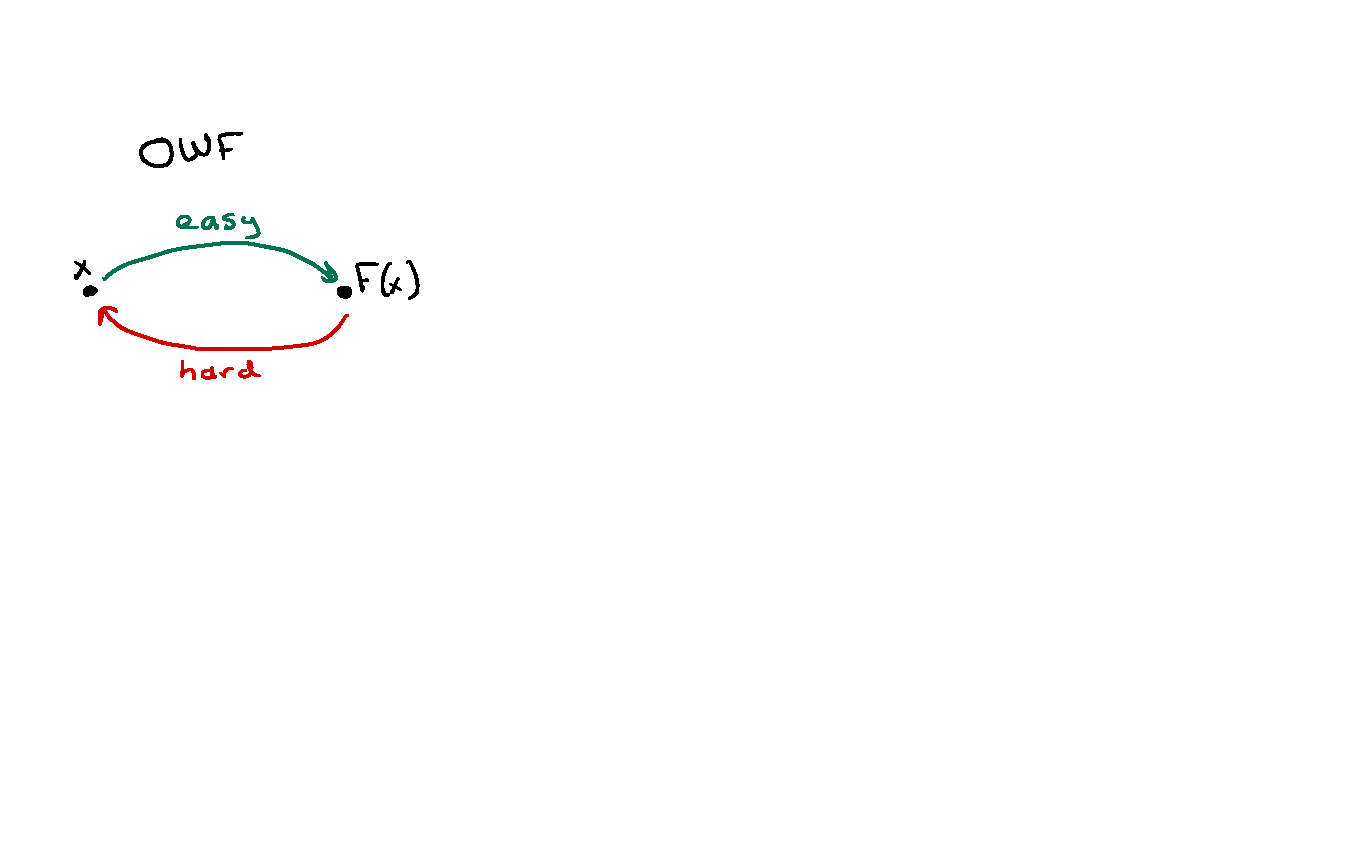
\includegraphics[width=0.45\textwidth]{figs/rsa-owf.pdf}
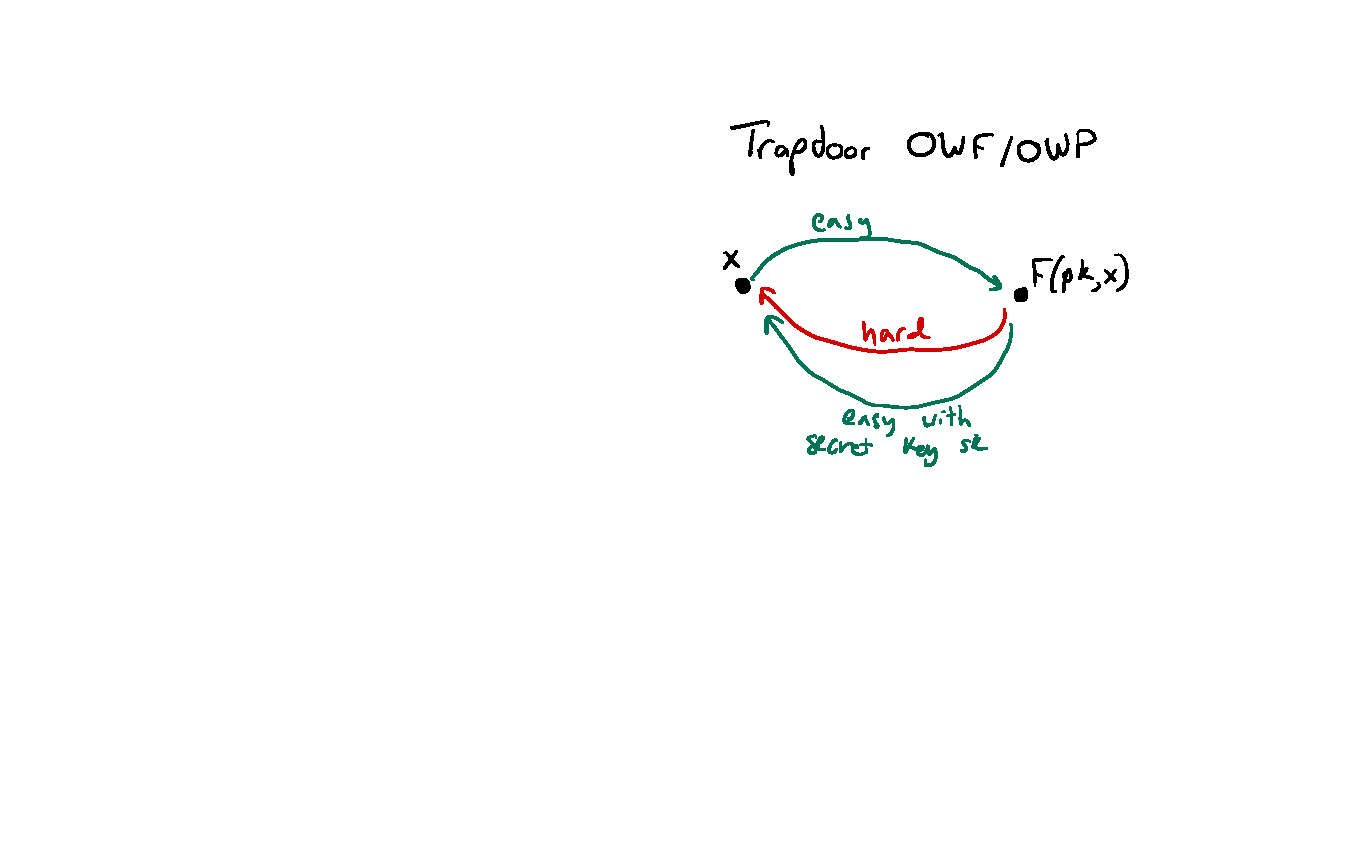
\includegraphics[width=0.55\textwidth]{figs/rsa-trapdoor.pdf}
\caption{A one-way function (at left) is hard to invert on random inputs.
A trapdoor one-way function/permutation (at right) is a function keyed
by a public key. The function is easy to invert given the secret key 
and is hard to invert otherwise.
}
\end{figure}

RSA implements a \emph{trapdoor one-way function}.
Informally, a trapdoor one-way function is a function that is
easy to compute in the forward direction but that is hard to 
invert \emph{except} to someone knowing a secret key.
So it is like a one-way function with a ``trapdoor'' that allows
efficient inversion.

RSA actually implements a trapdoor one-way \emph{permutation}---that is,
it maps an input space onto itself with no collisions.

\subsection{Definition}

Formally, a trapdoor one-way permutation over input space $\calX$ is a triple of
efficient algorithms:\marginnote{If we wanted to be completely formal, the
input space would be parameterized by the security parameter $\lambda$.
So we would have a family of input spaces $\{\calX_\lambda\}_{\lambda \in \N}$---%
one for each choice of $\lambda$. This way the input space can grow with~$\lambda$.}

\begin{itemize}
  \item $\Gen(1^\lambda) \to (\sk, \pk)$.
        The key-generation algorithm takes as input the security parameter $\lambda \in \N$,
        expressed as a unary string, and outputs a secret key and a public key.
  \item $F(\pk, x) \to y$.\marginnote{In the RSA construction, the input space $\calX$
depends on the public key, but we elide that technical detail here.}
        The evaluation algorithm $F$ takes as input the
        public key $\pk$ and an input $x \in \calX$, and outputs 
        a value $y \in \calX$.
  \item $I(\sk, y) \to x'$.
        The inversion algorithm $I$ takes as input the secret key $\sk$
        and a point $y \in \calX$, and outputs its inverse $x \in \calX$.
\end{itemize}

\paragraph{Correctness.}
Informally, we want that for keypairs $(\sk, \pk)$ output by $\Gen$,
we have that $F(\pk, \cdot)$ and $I(\sk, \cdot)$ are inverses of each other.
More formally, for all $\lambda \in \N$, $(\sk, \pk) \gets \Gen(1^\lambda)$, and $x \in \calX$,
we require:
\[ I(\sk, F(\pk, x))= x.\]

\paragraph{Security.}
Security requires that $F(\pk, \cdot)$ is hard to invert (in the sense of a one-way function)
on a randomly sampled input in the input space $\calX$, even when the adversary 
is given the public key $\pk$.
That is, for all efficient adversaries $\calA$, there exists a negligible function $\negl(\cdot)$
such that 
\[ \Pr\left[ 
\calA(\pk, F(\pk, x)) = x
\colon \begin{aligned}
  (\sk, \pk) &\gets \Gen(1^\lambda)\\
  x &\getsr \calX
\end{aligned}\right] \leq \negl(\lambda).\]

When we use the RSA cryptosystem, we make the assumption 
that the RSA function is hard to invert given only the public key:
\begin{defn}[RSA Assumption]
The RSA function $(\Gen, F, I)$ is a trapdoor one-way permutation.
\end{defn}

\paragraph{\textbf{IMPORTANT}:}
Just as a one-way function is only hard to invert on a \emph{randomly sampled input},
a trapdoor one-way function is only hard to invert on a randomly sampled input.
Many of the cryptographic failures of RSA come from assuming that the RSA
one-way function is hard to invert on non-random inputs.


\subsection{Digital signatures from trapdoor one-way permutations}

This construction is called ``full-domain hash.''\autocite{BR93}
The construction makes use of a hash function $H$ and resulting
signature scheme is secure, provided that we model the hash function~$H$
as a ``random oracle.''

In other words, to argue security, it is not sufficient to show that
$H$ is, for example, collision resistant.
Instead, we can only prove security provided that we pretend that $H$
is a truly random function---i.e., in the random-oracle model.
When we instantiate the hash function $H$ with some concrete cryptographic
hash function, such as SHA256, we hope that the resulting signature
scheme is still secure.
In practice, this approach works quite well.

One way to think about it is that if a signature scheme is secure
in the random-oracle model, then the concrete signature scheme
is in some sense secure against attacks that do not exploit the peculiarities
of the hash function.

\medskip 

In the construction, we use:
\begin{itemize}
  \item a trapdoor one-way permutation $(\Gen, F, I)$, and
  \item a hash function $H \colon \zo^* \to \calX$,
        which we model as a random oracle in the
        security analysis.
\end{itemize}

\paragraph{Construction.}
We construct a digital-signature scheme $(\Gen, \Sign, \Ver)$ as follows:
\begin{itemize}
  \item $\Gen$ -- Just run the key-generation algorithm for the
        trapdoor one-way permutation.
  \item $\Sign(\sk, m) \to \sigma$.
        Hash the message down to an element $h$ of the input space $\calX$
        of the trapdoor one-way permutation using the hash function $H$. Then invert
        the trapdoor one-way permutation at that point:
        \begin{itemize}
          \item Compute $h \gets H(m)$.
          \item Output $\sigma \gets I(\sk, h)$.
        \end{itemize}
      \item $\Ver(\pk, m, \sigma) \to \zo.$ 
        \begin{itemize}
          \item Compute $h' \gets H(m)$.
          \item Accept if $F(\pk, \sigma) = h'$.
        \end{itemize}
\end{itemize}

Notice that the use of a hash function here is \textbf{critical} to
security, since (in the random oracle) it means that forging a signature
is as hard as inverting $F$ on a random point in its co-domain.
Without the hash function, forging a signature is only as hard as 
inverting $F$ on an attacker-chosen point in its co-domain, which 
could be easy.

\paragraph{Correctness.}
For all $\lambda \in \N$, $(\sk, \pk) \gets \Gen(1^\lambda)$, and $m \in \zo^*$,
we have:
\begin{align*}
\Ver(\pk, m, \Sign(\sk, m)) &= 1\{ F(\pk, I(\sk, H(m))) = H(m) \}\\
&= 1\{ I(\sk, F(\pk, I(\sk, H(m)))) = I(\sk, H(m)) \}
\intertext{and by correctness of the trapdoor one-way permutation:}
&= 1\{ I(\sk, H(m)) = I(\sk, H(m)) \} = 1.
\end{align*}

\paragraph{Security.}
The intuition here is that if the adversary cannot invert $F$,
it cannot find the preimage of $H(m)$ under $F$ for any message
on which it has not seen a signature.
See \href{https://toc.cryptobook.us/book.pdf#page=550}{Boneh-Shoup Chapter 13.3}
for the full security analysis.

\section{The RSA construction: Forward direction}

The algorithms for 
key-generation and 
for evaluating the RSA permutation
in the forward direction are not too complicated.

In what follows, we present RSA with 
public exponent $e=5$.
The same construction works with many other choices of $e$,
just by replacing all of the ``5''s below with some other
small prime: 3, 7, 13, etc.
A popular choice of the public exponent $e$ in practice is $e=2^{16}+1$.
The complexity of computing the RSA function in the forward
direction scales with the size of $e$, so we prefer small
choices of $e$.

\begin{itemize}
  \item $\Gen(1^\lambda) \to (\sk, \pk)$.\marginnote{In practice,
    we usually take the bitlength of primes to be $\lambda=1024$
    or $\lambda = 2048$.}
  \begin{itemize}
    \item Sample two random $\lambda$-bit primes $p$ and $q$
      such that $p \equiv q \equiv 4 \pmod 5$.\marginnote{%
        Standard RSA implementations require
        the weaker condition that the public exponent $e$
        shares no prime factors with $p-1$ and $q-1$.
        Using the stronger condition here simplifies 
        the inversion algorithm.}
    \item Set $N \gets p \cdot q$.
    \item Output $\sk \gets (p, q)$, and $\pk = N$.
  \end{itemize}
  \item $F(\pk = N, x) \to y$.
\begin{itemize}
  \item The input space for the RSA function is \\
    $\calX = \Z^*_N$---the set of elements in $\{0, 1, 2, \dots, N-1\}$
    relatively prime to $N$.
    \item Output $y \gets x^5 \bmod N$.
\end{itemize}
\end{itemize}

\begin{remark}
The key-generation algorithm relies on us being able
to sample large random primes.
One perhaps surprising fact is that there are many many 
large primes.
In particular, if you pick a random $\lambda$-bit number,
the probability that it is prime is roughly $1/\lambda$.\marginnote{For more 
on this, look up the Prime Number Theorem.}

We can sample a random $\lambda$-bit prime by just
picking random integers in the range $[2^\lambda, 2^{\lambda + 1})$
until we find a prime.
We can test for primality in $\approx \lambda^4$ time using
the Miller-Rabin primality test.
We also need that there are infinitely many primes congruent to
$4 \bmod 5$, but fortunately there are.
Generating RSA keys is expensive---it can take
a few seconds even on a modern machine.
\end{remark}

Notice that computing the RSA function in the forward direction is
relatively fast: it just requires three multiplications 
modulo a 2048-bit number $N$. That is, to compute $x^5 \bmod N$, we compute:
\[ (x^2)^2 \cdot x = x^5\mod N.\]


\medskip

Before describing the RSA inversion algorithm, we discuss 
why the RSA trapdoor one-way permutation should be hard
to invert without the secret key.

\subsection{Why should the RSA function be hard to invert?}
To invert the RSA function, the attacker's is effectively given
a value $y \getsr \Z_N$ and must find a value $x$ such that $x^5 = y \bmod N$.
Or, put another way, the attacker's task is essentially the following:
\begin{itemize}
  \item \textbf{Given:} A polynomial $p(X) \deq X^5 - y \in \Z_N[X]$,
                        for $y \getsr \Z_N$.
  \item \textbf{Find:}  A value $x \in \Z_N$ such that $p(x) = 0 \in \Z_N$.
\end{itemize}

So the attacker must find the root of a polynomial modulo a composite integer~$N$.

The premise of RSA-style cryptosystems is that we only
know of essentially two ways to find roots of polynomials modulo $N$:
\begin{itemize}
\item \textbf{Factor $N$ into primes} and find a root modulo each of the primes.
      (We will say more on this in a moment.)
      Since the best algorithms for factoring run in time roughly $2^{\sqrt[3]{\log N}} = 2^{\sqrt[3]{\lambda}}$,
      this approach is infeasible at present without knowing the factorization of $N$.
      \marginnote{In \cref{sec:fact} we present a factoring algorithm that runs
      in sub-exponential time $2^{\sqrt{\log N \log \log N}}$.
}

\item \textbf{Find a root over the integers} and reduce it modulo $N$.\marginnote{Actually,
      it suffices to find a root over the rational numbers, but the distinction isn't important here.}
      For example, it is easy to find a root of polynomials such as:\\
\begin{align*}
  X + 4 &= 3 &&\mod N,&\\
  X + 2Y &= 5 &&\mod N,&\\
  X^2 &= 9 &&\mod N\text{, and}&\\
  X^2-3x+2 &= (X-2)(X-1) = 3 &&\mod N.
\end{align*}\marginnote{There are many clever attacks 
for solving polynomial equations modulo composites
that work in certain special cases, but for most purposes
these are the two known attacks.}
When $y \getsr \Z_N$, the probability that $y$ is a perfect
5-th power, and thus that there is an integral root to $X^5 - y$,
is $\sqrt[5]{N}/N \approx 2^{-4\lambda/5}$, which is negligible
in the security parameter~$\lambda$.
So solving this equation over the integers is a dead end.

\paragraph{Is inverting the RSA function as hard as factoring the modulus?}
No one knows---the question has been open since the invention of RSA.
We do know that finding roots of certain polynomial equations, such as
$p(X) \deq X^2 - y \bmod N$ for random $y \getsr \Z_N$ \emph{is} as 
hard as factoring the modulus $N$.
But for RSA-type polynomials, the answer is unclear.

\end{itemize}

\section{The RSA construction: Inverse direction}

To understand how the inversion algorithm works, we will need some
number-theoretic tools.


\subsection{Tools from number theory}
For a natural number $N$, let $\phi(N)$ denote the number of integers
in $\Z_N = \{1, 2, 3, \dots, N\}$ that are relatively prime to $N$.\marginnote{Two
natural numbers are \emph{relatively prime} if they share no prime factors.}
When $p$ is prime $\phi(p) = p-1$.
The function $\phi(\cdot)$ is called \emph{Euler's totient function}.

When $N=pq$ is the product of two distinct primes, $\phi(N) = (p-1)(q-1)$.
That is so because all numbers in $\Z_N$ are relatively prime to $N$ except
$N$ and the multiples of $p$ and $q$:
\[ p, 2p, 3p, \dots, (q-1)p,\ \ \ q, 2q, 3q, \dots, (p-1)q.\]
So there are $N - (q-1) - (p-1) - 1 = (p-1)(q-1)$ numbers
in $\Z_N$ relatively prime to $N$.

\begin{theorem}[Euler's Theorem]\label{thm:euler}
Let $N$ be a natural number. Then for all $a \in \Z^*_N$,
\[ a^{\phi(N)} = 1 \mod N.\]
\end{theorem}
\begin{proof}
Consider the sets $\Z^*_N$ and $\{ax \bmod N \mid x \in \Z^*_N\}$.
These sets are equal, so the product of the elements in the two
sets is equal.
Let $X \gets \prod_{x \in \Z^*_N} x \bmod N$.
Then 
\[ X = a^{\phi(N)}X \bmod N \quad \Rightarrow\quad 1 = a^{\phi(N)} \bmod N.\]
\end{proof}



\begin{lemma}\label{lemma:inv}
Let $p$ and $q$ be distinct primes congruent to $4$ modulo $5$.
Define the integer $d = \frac{\phi(N) - 4}{5} + 1$.
Then $5d \equiv 1 \bmod \phi(N)$.
\end{lemma}

\begin{proof}
Observe that
\[ p \equiv 4 \bmod 5 \quad \Rightarrow \quad \phi(N) - 4 \equiv 0 \bmod 5,\]
so $\frac{\phi(N) - 4}{5}$ is an integer and thus $d$ is well defined.
Then $5 d = \phi(N) - 4 + 5 = 1 \bmod \phi(N)$.
\end{proof}


\subsection{Inverting the RSA function}

With the number theory out of the way, we can now describe how
to invert the RSA function.
All we have to do is to show how to compute a fifth root of $y \bmod N$.

\begin{itemize}
  \item $I(\sk, y) \to x$.
\begin{itemize}
  \item The secret key $\sk$ consists of the prime factors $p,q$ of $N$.
        Recall that $\phi(N) = (p-1)(q-1)$.
  \item Compute the integer $d \gets \frac{\phi(N) - 4}{5} + 1$, as in
    \cref{lemma:inv}.\marginnote{%
    We sometimes call $d$ the \emph{private exponent} in RSA.}

  \item Return $y^d \bmod N$.
\end{itemize}
\end{itemize}

It is not obvious why the inversion algorithm is correct.
Say that $y = x^5 \bmod N$.
Then:
\begin{align*}
  y^d &= (x^5)^d &&\bmod N\\
      &= x^{5d} &&\bmod N\\
&= x^{k \cdot \phi(N) + 1} &&\bmod N, \qquad \text{for some $k \in \Z$, by \cref{lemma:inv}}\\
        &= x \cdot (x^{\phi(N)})^k &&\bmod N\\
&= x &&\bmod N, \qquad\text{by \cref{thm:euler}}.\\
\end{align*}
We could write $5d = k \phi(N) + 1$ because from \cref{lemma:inv},
we know that $5d \equiv 1 \bmod \phi(N)$.

\paragraph{Using other public exponents.}
For our RSA-inversion algorithm to work, we need only to
compute the multiplicative inverse $e$ modulo $\phi(N)$.
That is, we need to compute an integers $d$ such that
$ed \equiv 1 \bmod \phi(N)$.
Such an inverse always exists when $e$ and $\phi(N)=(p-1)(q-1)$ are
relatively prime.
RSA implementations typically use the extended Euclidean
algorithm to compute the multiplicative inverse of $e$ modulo $\phi(N)$.
That algorithm is more general, but the one we used in \cref{lemma:inv}
is simpler and is self-contained.

\paragraph{Inverting RSA is easy on a negligible fraction of points.}
Recall the RSA is 
If the preimage under the RSA function of a point $y$ is very very small,
then 
If $x < N^{1/5}$, then computing $x$ given $y = x^5 \bmod N$ is \emph{easy}.


\paragraph{Is inverting RSA as hard as factoring the modulus $N$?}
The inversion algorithm we showed here requires knowing the prime factors
of the modulus $N$.
Inverting RSA is thus \emph{no harder than} factoring $N$.

Is inverting RSA \emph{as hard as} factoring $N$?
In particular, if we have an efficient algorithm $\calA$ that inverts
RSA, can we use $\calA$ to factor the modulus $N$?
No one knows!

Most cryptographers, I would guess, believe that inverting the RSA function
is as hard as factoring.
But for all we know, it could be that computing fifth roots modulo $N$ is \emph{easier}
than factoring the modulus.



\chapter{Public-key Infrastructure}

In the last chapter, we discussed digital
signatures, which allow us to authenticate messages
without a shared secret.
For example, if I have the public signature-verification key 
of the university dean, I can verify that signed emails from 
the dean really came from her and not from someone pretending to be her.
But to verify the signature on the dean's message, I need to know her
signature-verification key $\vk$.
How can I (the recipient) obtain this verification key without
a secure channel to the dean (the sender)?

Unfortunately, there are no perfect solutions to this problem.
In this section, we will discuss some of the approaches that
we use in practice.

\section{Public-key infrastructure}

The goal of a public-key infrastructure is to facilitate
the mapping of \textbf{human-intelligible names} to
\textbf{signature-verification keys}.
Examples of human-intelligible names that we map to keys
are: email addresses, domain names, legal entities, phone numbers, and
usernames (e.g., within a company).

We can think of the public-key infrastructure as implementing
the following (grossly simplified) API:
\[ \mathsf{IsKeyFor}(\vk, \texttt{name}) \to \zo.\]
That is, given a verification key $\vk$ and a name $\texttt{name}$, 
the public-key infrastructure gives a way to check whether this mapping
is valid.

% TODO: exmaples: chisel, meet in person, trusted source, blockchain

We now discuss some ways to implement this API.

\section{Option 1: Use verification keys as names}
One option is to just refer to everyone by the bytes of
their signature-verification key.
This way, there is no need to do a messy name-to-verification-key 
translation at all.

This is not practical for humans generally: it would be difficult
to remember your friends' names if you had to call them by 
random 32-byte strings!
However, some digital services such as Bitcoin indeed use verification
keys as identities: when you want to transfer Bitcoin to someone,
you send the coins to an account identified by their public key.
The public key \emph{is} name of that account.

Using keys as names has a two major problems:
\begin{itemize}
	\item Verification keys are hard to remember. Things like email addresses, domain names, kerberos usernames, phone numbers, and so on, are much easier for humans to remember.
	\item There is no way to update the name-to-key mapping. If you lose the secret key associated with your name/account, there is no way to ``update'' the key to a new value. In practice, people lose their secret keys all the time, so supporting key updates is critical in most systems.
\end{itemize}

% TODO: this introduction does not flow very well
% it might be good to have a section elaborating on the need to change keys a bit more.

\section{Trust on first use (TOFU)}
Another strategy is to avoid having any global mapping from names to verification keys.
Instead, a client can just accept the first verification key 
that it sees associated with a given name.
The secure shell system (\ttt{SSH}) uses TOFU for key management by default.

In particular, the key-validation logic looks like this:

\begin{framed}
\noindent
$\mathsf{keymap} \gets \{ \}$.

\medskip
\noindent
$\mathsf{IsKeyFor}(\vk, \texttt{name}):$ 
\begin{compactitem}
\item If $\mathsf{keymap}[\texttt{name}]$ is undefined:
      \begin{compactitem}
      \item Set $\mathsf{keymap}[\texttt{name}] \gets \vk$.
      \item Return true..
      \end{compactitem}

\item Else: Return $\mathsf{keymap}[\texttt{name}] == \vk$.
\end{compactitem}
\end{framed}

That is, the client will accept the \emph{first} verification key 
it sees associated with a particular name.
Later on, the client will only accept the same verification key
for that name.

TOFU is very simple to implement and provides a meaningful security
guarantees. 
There are two drawbacks:
\begin{itemize}
  \item If the first key that client receives for a particular name 
        is incorrect/attacker-generated, the attacker can forge signatures
        under that name.
  \item It is not clear with TOFU how to handle key updates. In most systems that use TOFU, whenever the sender's key changes, the system notifies the user and allows them to accept or reject the new key. The burden is then on the user to figure out whether the sender really did change their signing keypair, or whether there is an attack in progress.
\end{itemize}

\section{Certificates}
Another option is to rely on a few parties to
manage the mapping of names to public keys.
These entities are called \emph{Certificate Authorities} (CAs).
Your operating system and web browser typically come bundled with a
set of roughly 100 public signature-verification keys, owned by 
each of 100 CAs.

Whenever the owner of website \ttt{example.com}, for example, generates 
a new public key $\vk_\ttt{example.com}$, the website owner can ask a 
certificate authority to certify that $\vk_\ttt{example.com}$ really belongs to \ttt{example.com}.
The certificate authority does this by signing the
pair $(\ttt{example.com}, \vk_\ttt{example.com})$
using its own signing keypair $\vk_\text{CA}$
to generate a signature $\sigma_\text{CA}$.
This signed attestation $(\ttt{example.com},\allowbreak \vk_\ttt{example.com},\allowbreak \sigma_\text{CA})$
is called a \textit{certificate}.
\marginnote{In practice the structure of certificates is much more complicated
than we are showing here, and include all sorts of additional metadata. But the 
basic idea is the same as we describe here.}

When a client connects to \ttt{example.com}, the server at \ttt{example.com}
will supply the client with the certificate $(\ttt{example.com},\allowbreak \vk_\ttt{example.com},\allowbreak\sigma_\text{CA})$.
As long as this certificate was signed by a CA that the client trusts (i.e., 
a CA for which the client has a verification key),
the client can validate the certificate and conclude that 
the verification key $\vk_\ttt{example.com}$ really belongs to \ttt{example.com}.

In pseudocode the logic for verifying certificates looks like this:
\begin{framed}
\noindent
$\mathsf{caKeys} \gets \{\vk_\text{Verisign}, \vk_\text{Let's Encrypt}, \dots \}$.

\medskip
\noindent
$\mathsf{IsKeyFor}((\vk, \sigma), \texttt{name}):$ 
\begin{compactitem}
\item For each $\vk_\text{CA}$ in $\mathsf{caKeys}$:
      \begin{compactitem}
      \item If $\Ver(\vk_\text{CA}, (\texttt{name}, \vk), \sigma) = 1$: Return true.
      \end{compactitem}
\item Return false.
\end{compactitem}
\end{framed}

A very nice feature of certificate-based public-key infrastructure is that
the client does not need to communicate with the CA to validate a 
name-to-key mapping. The client only needs to perform one signature-verification
check.
\marginnote{In order to use TLS on a website you own, you need to convince one of the certificate authorities to give you a certificate---i.e., to sign your $(\ttt{name}, \vk)$ pair. 
To do so, the CA will have some protocol to follow---typically, you will send your $(\ttt{name}, \vk)$ pair to the CA, who will then ask you to verify that you own the name somehow. This is called \textit{domain validation}.
In the case of web certificates, the CA may verify ownership by requiring you to upload a file file to your server, to add a new DNS record with a random value, or something similar.
Once the CA is convinced that you own the domain, the CA will reply with a certificate: a signature over the tuple $(\ttt{name}, \vk)$. This $(\ttt{name}, \vk, \sig_{\text{CA}})$.
}

Certificates in practice works quite well:
\begin{itemize}[noitemsep]
	\item The client only needs to store $\approx 100$ CA verification keys,
        and yet the client can validate the name-to-key mappings for millions of websites.
	\item A client can choose which CAs to trust 
        (though in practice, clients typically delegate this decision to software vendors).
	\item The client never needs to interact with the CA.
\end{itemize}

However, certificates still have some drawbacks:
\begin{itemize}[noitemsep]
  \item If an attacker compromises \emph{any} CA, they can generate certificates for any domain.
	\item Certificate authorities often perform quite minimal validation of domain ownership.
	\item If a server's private key gets stolen, 
        there is no great plan for \emph{revoking} or updating a name-to-key mapping.
\end{itemize}

\subsection{Domain Validation}

Domain Validated (DV) certificates are quite common. CA validation uses a simple technical check for domain ownership. For example, the CA asks the requester amazon.com to put a nonce in a file on an amazon.com server. Then, the CA retrieves that file, and checks the nonce. The (reasonable) assumption is that only the server owner could have created such a file. Alternately, the CA could ask the requester to create certain Domain Name Services (DNS) records under amazon.com, e.g., acme-challenge.amazon.com.

This check is often automated, and is fast, convenient, cheap. An example DV CA is {\bf Let's Encrypt}. It is easy to use and free; the requester doesn't have to be a real company.

DV certificates only have low-level DNS ownership guarantees: "CA validated that owner of certificate owns amazon.com". However, the guarantee closely matches what CAs can be expected to validate in real life. 

A standard protocol for validating domain ownership is ACME\footnote{https://tools.ietf.org/html/rfc8555\#section-8.3}.

\subsection{Revocation}
In many cases, a CA will want to delete or change a name-to-key mapping.
This process is called \emph{certificate revocation}.
There are several possible reasons for this:
\begin{itemize}[noitemsep]
	\item The owner of a verification key may have their corresponding secret key
        be lost or stolen.
	\item A company may want to rotate keys, 
        for example to update to a new cryptographic algorithm.
	\item A website may go out of business and another entity buys their domain name.
	\item Software bugs may lead a user to generate an
        insecure keypair that they later want to revoke.\autocite{yilek2009private,nemec2017return}
\end{itemize}

In a scheme that uses certificates, this seems like a hard problem: since there is no interaction with the CA to verify a certificate, there is no way for a CA to \textquote{take back} a certificate. There are again no excellent solutions to this, but there are a few strategies used in practice.

\paragraph{Expiration Dates}
One pragmatic way to handle revocation is to add
an expiration date to each generated
certificate---if this expiration date has passed,
the client will reject the certificate. This way,
a server will need to re-authenticate to the CA
that they own the name that they claim to own
periodically. So, for example, an attacker that steals
a website's secret key will only be able to use it 
until the certificate expires.
In practice, certificates used on the Internet
typically expiration dates between 90 days 
and 1-2 years.

\paragraph{Software Updates}
Another solution is for the browser (or client, more generally)
to maintain a list of revoked certificates.
On every connection, the browser will check whether the provided certificate is in this local revocation list and refuse it if so.
Since browsers today check for updates very frequently, this strategy can respond to a stolen secret key quickly. However, there is a large storage cost since now every browser needs to store this (potentially large) list of revoked certificates.

\paragraph{CA Revocation List}
To avoid depending on browser manufacturers to update this revocation list, another strategy is to ask the CA for it directly. One way to do this is similar to the above: periodically query the CA to download its updated revocation list and check that each certificate is not in this list. This method has fallen out of favor, in part because clients (e.g., behind corporate firewalls) cannot connect directly to the CAs to download these revocation lists.



\part{Transport Security}

\chapter{Introduction to Encryption}

So far, we have explored methods for authenticating data---verifying that it has not been modified in transit.
However, the integrity-protection mechanisms we
have discussed provide no \emph{confidentiality}:
a network eavesdropper can still view everything that 
we send over the network.

In this chapter, we will discuss \emph{encryption},
which allow two parties to exchange messages over an insecure
network while hiding the contents of their communications.

% TODO: demo of tcpdump output would be cool

We will cover encryption in a sequence of steps:
\begin{itemize}
  \item First, we will construct an encryption scheme with a \emph{weak form of security} for \emph{fixed-length messages} for settings in which the sender and recipient have a \emph{shared secret key}.
  \item Next, we will show how to extend this scheme to support \emph{variable-length messages}.
  \item Then, we will show how to improve the scheme to have a \emph{strong form of security}.
  \item Finally, we will show how to implement encryption in settings in which the sender and recipient \emph{have no shared secrets}.
\end{itemize}
At the conclusion of this part, we will discuss how deployed systems
use encryption, and 
we will think about some problems that encryption does not solve.

\section{Background}

\paragraph{The need for encryption}
The internet is a massive network of wifi access
points, routers, switches, undersea cables, DNS
servers, and much more.
There are many, many
devices for a potential adversary to compromise
and many vantage points from which an attacker can 
observe network traffic. Every single hop your
packets take is a potential point of compromise.

To make matters worse, most standard network protocols provide \emph{no authentication or encryption}: in Ethernet, IP, DNS, 
email, HTTP, and others, an adversary is free to modify and read the traffic we send and receive. 
Protecting confidentiality typically requires augmenting these standard network
protocols with some form of authentication and encryption.

\paragraph{Systems using encryption}
Encryption shows up in a large number of deployed systems. A few examples are:
\begin{itemize}
  \item \textbf{Messaging apps}, such as WhatsApp, Signal, and iMessage, encrypt
        traffic between app users so that the server cannot easily read it.
  \item \textbf{Network protocols}, such as SSH and HTTPS use encryption to 
        protect traffic between a service's clients and servers.
  \item \textbf{File-storage systems} use encryption to protect data at rest.
        So if a thief steals your laptop, they will not easily be able to read
        the encrypted files on your hard disk.
\end{itemize}

\section{Encryption Scheme Syntax}
Encryption schemes are defined with respect to a key space $\calK$, a message space $\calM$, and a ciphertext space $\calC$.
For now, think of $\calK = \calM = \zo^n$ and $\calC = \zo^{2n}$,
for a security parameter $n$.\marginnote{Remember that in practice,
we will often take the size of the keyspace $\abs{\calK}$ to be at least
$2^{128}$ to prevent brute-force key-guessing attacks.} 
An encryption scheme then consists of two algorithms:

\begin{itemize}
	\item $\Enc: \calK \times \calM \rightarrow \calC$
	\item $\Dec: \calK \times \calC \rightarrow \calM$
    \marginnote{As we will see later on, the decryption algorithm 
    $\Dec$ can sometimes output \textquote{FAIL} or $\bot$.}
\end{itemize}

The definition of correctness for an encryption scheme just states
that if you encrypt a message $m$ with a key $k$, and then you decrypt
the resulting ciphertext with the same key $k$, you end up with the 
same message $m$ that you started with:
\begin{definition}[Encryption Scheme, Correctness]
An encryption scheme is correct if, for all keys $k \in \calK$ and all messages $m \in \calM$, $\Dec(k, \Enc(k, m)) = m$.
\end{definition}

Defining security for encryption scheme is tricky business.
Many of the most obvious security definitions are insufficient:
\begin{itemize}
  \item \textbf{Bad definition:} \emph{``An encryption scheme is secure 
        if it is infeasible for an attacker to recover the plaintext
        message given only a ciphertext.}
        This definition admits encryption schemes in which the ciphertext
        leaks half of the plaintext bits.
  \item \textbf{Bad definition:} \emph{``An encryption scheme is secure 
        if it is infeasible for an attacker to recover any bit of
        the plaintext message given only a ciphertext.}
        This definition admits encryption schemes in which the ciphertext
        leaks the parity of the plaintext bits.
\end{itemize}

The starting-point (weak) security definition we will use
is called \emph{indistinguishability under adaptive chosen plaintext attack}
($\INDCPA$).
Intuitively, a scheme is CPA-secure if an attacker cannot tell which of two chosen messages are encrypted, even after seeing encryptions of many attacker-chosen messages.

\begin{definition}[Encryption Scheme, CPA Security (weak)]\label{defn:cpa}
Formally, an encryption scheme $(\Enc, \Dec)$ over message space $\calM$
and key space $\calK$ is CPA-secure if 
all efficient adversaries win
the following game with probability at most $\tfrac{1}{2}$ + ``negligible:''
  \begin{itemize}[noitemsep]
		\item The challenger samples $b \rgets \bin$ and $k \rgets \calK$.
    \item Polynomially many times: \quad \emph{// Chosen-plaintext queries}
          \begin{itemize}
            \item The adversary sends the challenger a message $m_i \in \calM$
            \item The challenger replies with $c_i \gets \Enc(k, m_i)$.
          \end{itemize}
    \item The adversary then sends two messages $m^*_0, m^*_1 \in \calM$ to the challenger.
          (We require $\abs{m^*_0} = \abs{m^*_1}$.)
          \marginnote{Standard encryption systems do not hide the
          length of the message being encrypted.
          So, if the message space $\calM$ contains messages of different
          lengths, our security definition requires the adversary to distinguish
          the encryption of two messages of the \emph{same} length.}

    \item The challenger replies with $c^* \gets \Enc(k, m^*_b)$.
		\item The adversary outputs a value $b' \in \bin$. The adversary wins if $b=b'$. 
	\end{itemize}
\end{definition}

One potentially surprising consequence of the CPA-security definition 
for encryption schemes is:
\begin{center}
\emph{For an encryption scheme to be secure in any meaningful sense,\\
the encryption algorithm \textbf{must} be randomized}.
\end{center}\marginnote{In contrast, secure MACs can be---and typically are---deterministic!}

If the encryption algorithm is deterministic (i.e., not randomized),
an attacker can win the CPA security game in \cref{defn:cpa}
with probability 1.
To do so:
\begin{itemize}[noitemsep]
  \item The attacker first asks for encryption of a message $m_0$
and receives a ciphertext $c_0$.
  \item Then, the attacker attacker choose a message $m_1 \neq m_0$ and
sends $(m^*_0, m^*_1) = (m_0, m_1)$ to the challenger
and receives the challenge ciphertext $c^*$.
  \item If $c^* = c_0$, the attacker outputs 0.
Otherwise, the attacker outputs 1.
\end{itemize}

Deterministic encryption schemes are not only broken in theory,
they are also broken in practice.
For example, if you encrypt the pixels of an image using a deterministic
encryption scheme, the encrypted image essentially reveals the plaintext image.

\paragraph{Why CPA security is a ``weak'' form of security}
There are two reasons why CPA security is a weak or insufficient 
definition of security for an encryption scheme:
\begin{itemize}
  \item First, the CPA security definition
    guarantees nothing about message
    \emph{integrity}: an attacker can modify the
    ciphertext and potentially change the meaning
    of the encrypted message in a meaningful way
    (even if the attacker does not know the encrypted message!).
  \item Second, the CPA security definition guarantees
    nothing in the event that the adversary can obtain
    \emph{decryptions} of ciphertexts of its choosing.
    In practice, attackers can often obtain decryptions
    of chosen ciphertexts.
    for example, in a system where a client sends encrypted messages to a server and the server does something in response, an attacker can send encrypted queries to the server and observe its behavior to learn some function of the decrypted contents of the message. Later on, we will expand our definition to include these \textit{chosen ciphertext attacks}.
\end{itemize}

\section{One-time Pad}
The one-time pad is perhaps the simplest encryption scheme.
Its keyspace, message space, and ciphertext space are all the set of $n$-bit strings.
The algorithms are then:
\begin{itemize}
  \item $\Enc(k, m) \to c$. Compute $c \gets (k \oplus m)$.
  \item $\Dec(k, c) \to m$. Compute $m' \gets (k \oplus c)$.
\end{itemize}

The encryption scheme is correct since $\Dec(k, \Enc(k, m)) = k \oplus (k \oplus m) = m$.
A less obvious fact is that it is also \emph{one-time secure}:
if an attacker sees only one message with encrypted a one-time-pad key $k$,
it learns nothing about the underlying plaintext.
\marginnote{The one-time pad is actually one-time secure in a very strong sense:
it protects confidentiality even against a computationally unbounded attacker---one
that can perform arbitrary amounts of computation.}

\paragraph{The ``two-time pad'' attack}
The one-time pad is insecure if the same key $k$ is every used to 
encrypt two messages.
In particular, if two ciphertexts are ever computed using the same key, we
have:
\begin{align*}
  c_1 &= k \xor m_1 \\
  c_2 &= k \xor m_2 \\ 
  c_1 \oplus c_2 &= (k \xor m_1) \xor (k \xor m_2) = m_1 \xor m_2.
\end{align*}
The attacker then learns the XOR of the two encrypted messages,
which is often enough to leak all sorts of sensitive information
about the plaintext.
For example, if the attacker knows some bits of $m_1$, it can learn
some bits of $m_2$.

\paragraph{Why the one-time pad is useful}
The one-time pad encryption scheme feels in some sense useless: if a secure channel exists through which Alice and Bob can exchange an $n$-bit secret key, they may as well use that channel to exchange the message itself!
There is some merit still in the one-time pad: it is possible
to exchange the key ahead of time, and then send encrypted messages
later on.
Diplomats indeed used the one-time pad in this way throughout the 20th century.
They would exchange huge books of keying material (random strings) 
and then use these keys to communicate securely over long distances.

In practice, it is much more convenient to be able to exchange a \emph{short}
key and then use it to encrypt many \emph{long} messages.

\section{A Weak Encryption Scheme}\label{sec:lec8:weakenc}
What we effectively need is a way to generate many bits of random-looking keys 
(i.e., keys for the one-time pad encryption scheme)
from a single short random string.

To generate this, we can use a pseudorandom function! 
\marginnote{If you forget what a pseudorandom function is, refer back to \cref{defn:prf}.}
In particular, we would like a pseudorandom 
function of the form $F \colon \bin^n \times \bin^n \rightarrow \bin^n$. 
\marginnote{In practice, we will use AES or another block cipher
as a pseudorandom function, so we will have $n = 128$ or so.}

Using such a pseudorandom function, we can construct a new 
encryption scheme that replaces the truly random keys 
with pseudorandom keys generated from the pseudorandom function.
The keyspace and message space for this encryption space are $\zo^n$
and the ciphertext space is $\zo^{2n}$.
The algorithms are:
\begin{itemize}
	\item $\Enc(k, m) \to c$:
      \begin{itemize}
        \item Sample a random value $r \rgets \bin^n$.
              We call this the ``nonce.''
        \item Compute a one-time key $k \gets F(k, r)$ using the pseudorandom function.
        \item Use this key to compute the ciphertext using the one-time pad: 
          output $c \gets (r, k \xor m) \in \zo^{2n}$.
      \end{itemize}
	\item $\Dec(k, c)$:
        \begin{itemize}
          \item Parse the ciphertext $c$ into $(r, c')$.
          \item Compute $m \gets c' \xor F(k, r)$.
        \end{itemize}
\end{itemize}
\marginnote{While this encryption scheme is CPA-secure,
it provides no message integrity.
For any string $\Delta \in \zo^n$,
an attacker can modify a ciphetext $(r, c')$ to $(r, c' \oplus \Delta)$.
This ciphertexts now decrypts to the original message XORd
with the attacker-chosen string $\Delta$.
}

Correctness holds by construction.
The security argument goes in three steps:
\begin{itemize}
  \item First, we argue that if $n$ is large enough, the probability 
        that the encryption algorithm ever chooses the same $r$ value twice
        is negligible.
        \marginnote{By the Birthday Paradox, after encrypting $T$ messages,
        the probability of a repeated $r$ value is $O(T^2/2^n)$,
        which is negligible in the key length~$n$.}
  \item Second, we argue that as long as the encryption algorithm
        never chooses the same $r$ value twice, 
        we can replace the values $F(k, r)$ with truly random strings.
        By the security of the pseudorandom function, the adversary will
        not notice this change.
  \item At this point, we can appeal to the security of the one-time pad scheme
        to argue that the adversary has no chance of winning the security 
        game (\cref{defn:cpa}).
\end{itemize}

For security to hold, it is crucial that the probability 
that the encryption algorithm uses the same encryption nonce $r$ twice
be negligibly small.
If the encryption algorithm ever selects the
same random nonce $r$ twice, the pad $F(k, r)$ will be identical in 
two ciphertexts.
An attacker can then apply the two-time-pad attack to recover the XOR of the two messages.

By the Birthday Paradox, if we sample the nonce from a space of size $2^{128}$, we can expect a collision in 128-bit random values once around $2^{64}$ have been generated. Therefore, any single encryption-key must be used for $\ll 2^{64}$ messages.
Cryptographic standards typically limit the number of bytes that users can
encrypt with the same key to prevent these sorts of problems.


\section{Encrypting longer messages: Counter mode}
\label{sec:enc:ctr}

The CPA-secure encryption scheme of \cref{sec:lec8:weakenc} only
allowed encrypting messages of a fixed length.
We now show how to use \emph{counter-mode encryption} to extend
this scheme to support messages of arbitrary length.
That is, we will construct an encryption scheme 
$\Enc \colon \calK \times \zo^* \to \zo^*$
for messages of any length.
\marginnote{In practice, encryption schemes place some
(large) bound on the length of encrypted messages.
For example, the AES-GCM cipher has a maximum message
limit of just under 64 GiB.
}

Counter-mode encryption works much as the CPA-secure encryption
scheme we have already seen in \cref{sec:lec8:weakenc}, except 
that we split the message into blocks and encrypt each block separately.

\newcommand{\ToString}{\mathsf{ToString}}
We will use the function $\ToString \colon \{0, \dots, 2^n-1\} \to \zon$,
which converts an integer in $\{0, \dots, 2^n -1\}$ to an $n$-bit string in the natural way.

The encryption scheme uses a pseudorandom function $F \colon \calK \times \zon \to \zon$.
The secret encryption key is a key $k \in \calK$ for the pseudorandom function.
To encrypt a message, we choose a fresh random value $r \getsr \{0, \dots, 2^n-1\}$ and 
XOR the $i$th block of the message with the value $F(k, \ToString(r+i \bmod 2^n))$.

\begin{itemize}
  \item $\Enc(k, m):$
    \begin{itemize}
      \item Split the message $m$ into blocks of $n$ bits: $(m_1, m_2, m_3, \dots, m_\ell)$.
            The last message block $m_\ell$ may be shorter than $n$ bits.
      \item Sample a random nonce 
            $r \getsr \{0, \dots, 2^n-1\}$.
        \marginnote{The nonce is sometimes called an ``initialization vector'' or ``IV.''} 
      \item For $i = 1, \dots, \ell$: Compute $c_i \gets m_i \oplus F(k, \mathsf{ToString}(r+i \bmod 2^n))$.\\
            (If the last message block $m_\ell$ is less than $n$ bits long, 
            truncate the last ciphertext block $c_\ell$ to the length of $m_\ell$.)
      \item Output the ciphertext $c = \big(r, c_1, \dots, c_\ell)$.
    \end{itemize}

  \item $\Dec(k, c):$
    \begin{itemize}
      \item Parse the ciphertext $c$ as $(r, c_1, \dots, c_\ell)$,
            where all values but the last are exactly $n$ bits long.
          \item For $i = 1, \dots, \ell$: Compute $m_i \gets c_i \oplus F(k, \ToString(r+i \bmod 2^n))$.
            (Truncate $m_\ell$ to the length of $c_\ell$.)
      \item Output the message $m = (m_1 \| \dots \| m_\ell)$.
    \end{itemize}

\end{itemize}

As long as the space of random values $r$ is large enough to ensure that
the encryption routine never evaluates the pseudorandom function $F(k, \cdot)$
on the same input twice, this scheme will be CPA secure.

You may notice that this encryption scheme reveals
the length of the encrypted message to the attacker! This
indeed is a potential risk, but in some sense it
is required: if we were to hide the length of the
message, we would need to set some maximum message
length and pad it up to this length. If we did
this, encrypting a single word would necessarily
result in a ciphertext equal in length to the
ciphertext of encrypting a movie! This would
greatly decrease the practicality of our
encryption scheme. For applications where hiding
the length is especially important, the messages
can be padded to ensure they are all the same
length before they are passed to the encryption
scheme.


\chapter{Authenticated Encryption}

We have just constructed an encryption scheme with
weak (CPA) security: one that provided security
given that the adversary could see
\emph{encryptions} of messages of her choice.
The ``gold standard'' security notion for encryption
schemes allows the attacker to receive both encryptions
of messages of its choice 
\emph{and} decryptions of ciphertexts of its choice.
Our security notion then says that 
even an attacker with this power should not be
able to distinguish which of two chosen plaintext
message a given ciphertexts encrypts.
This new and strong notion of security for encryption
schemes is called 
\emph{security against adaoptive chosen-ciphertext attacks}.

\paragraph{Motivation: Chosen-ciphertext security}
It is not clear why chosen-ciphertext security is the right 
security notion to consider. 
In real-life applications, why would we ever allow an attacker
to obtain \emph{decryptions} of ciphertexts of its choosing?
It turns out that, in many settings, attackers can indeed
trick honest parties into decrypting adversarially ciphertexts
and revealing their contents.

As a simple example, imagine a server that receives encrypted
requests from the network, decrypts them, and either:
\begin{itemize}
  \item returns an error if the decrypted request is malformed, or
  \item silently processes the request otherwise.
\end{itemize}
In this case, an attacker can send ciphertexts to the server and
learn information about their decryptions by noticing whether or not
the server returned an error message.
\marginnote{If the server returns an error when the decrypted message
is illformed, we often call it a \emph{padding oracle}.
Many many real-world protocols using non-chosen-ciphertext-secure encryption
schemes fall victim to this sort of attack.}

CPA-secure encryption schemes provide \emph{no} security guarantees
in this setting. Even if the server leaks a single bit to the attacker 
about the
decrypted value (such as whether the decrypted ciphertext is a
well-formed request or not), the attacker could potentially learn 
the entire secret key!

As a concrete application-level example, consider what could
happen if SSH (the secure shell protocol) used the counter-mode
encryption scheme, as described in the previous lecture, without any
authentication.  A user might send the command
\texttt{echo secret > secret-file} to write their secret string,
\texttt{secret}, to their own private file \texttt{secret-file}.
The encryption of this command, sent over the network, would be the XOR
of the command and the PRF-generated pseudorandom bytes.  Suppose that
the adversary knows the user is running this command, but doesn't know
the contents of the 6-byte secret string.  Consider what
happens if the adversary XORs the encrypted message with the hexadecimal
bytes \texttt{00 00 00 00 00 00 00 00 00 00 00 00 00 00 5c 11 0e 02 4a
04 58 04 05 05 06}.  The leading zeroes mean that the first part of the
command, \texttt{echo secret > }, will remain unchanged.  When the server
decrypts the latter part of the command (originally \texttt{secret-file}),
however, it will obtain the XOR of \texttt{secret-file} and the bytes that
the adversary XOR'ed in, which happens to turn into the string \texttt{/tmp/public}.
As a result, if the server now runs this command, the user's secret data
will be written to a file \texttt{/tmp/public}, which might be available
to an adversary that also has an account on that same server and can look
at files in \texttt{/tmp}.

Chosen-ciphertext security guarantees that such attacks are ineffective.


\section{Defining Authenticated Encryption}

Authenticated-encryption schemes simultaneously provide message 
integrity (as a MAC does) and confidentiality (as CPA-secure encryption does).
Additionally, authenticated-encryption schemes remain secure even when 
an attacker can see encryptions and decrypts of ciphertexts of her choice.
Perhaps unsurprisingly, the standard way to construct an authenticated-encryption
scheme is to combine a CPA-secure encryption scheme with a MAC in a careful way.

We now formally define our strong security notion:
\emph{indistinguishability under chosen ciphertext attacks}, 
also known as IND-CCA2 security or CCA security.

\begin{definition}[CCA security for encryption (strong)]\label{defn:cca}
An encryption scheme is \emph{secure against 
adaptive chosen-ciphertext attacks}
if every efficient adversary wins the following 
game with probability at most $\tfrac{1}{2} + \text{\textquote{negligible}}$:

  \begin{itemize}[noitemsep]
		\item The challenger samples $b \rgets \bin$ and $k \rgets \calK$.
    \item The adversary can make either of the following queries to the challenger
      repeatedly:
      \begin{itemize}
    \item \emph{Chosen-plaintext queries}
          \begin{itemize}
            \item The adversary sends the challenger a message $m_i \in \calM$
						\item The challenger replies with $c_{m_i} \gets \Enc(k, m_i)$.
          \end{itemize}
    \item \emph{Chosen-ciphertext queries}
          \begin{itemize}
						\item The adversary sends the challenger a \emph{ciphertext} $c_j \notin \set{c_{m_0}, \ldots, c_{m_i}}$
						\item The challenger replies with $m_{c_j} \gets \Dec(k, c_j)$.
          \end{itemize}
      \end{itemize}
    \item The adversary then sends two messages $(m^*_0, m^*_1) \in \calM^2$ to the challenger,
          where $\abs{m^*_0} = \abs{m^*_1}$.
    \item The challenger replies with $c^* \gets \Enc(k, m^*_b)$.
    \item The adversary can make more chosen-plaintext queries
      and more chosen-ciphertext queries. (The adversary may not
      make a chosen-ciphertext query on the challenge ciphertext $c^*$.)
		\item The adversary outputs a value $b' \in \bin$.
    \item The adversary wins if $b=b'$. 
	\end{itemize}
\end{definition}


\subsection{Encrypt then MAC}
We typically achieve CCA security using the ``encrypt-then-MAC'' construction:
\begin{itemize}
  \item First, encrypt the message using a CPA-secure encryption scheme on key $k_\mathsf{Enc}$.
  \item Next, MAC the \emph{ciphertext} using a secure MAC scheme and an independent key 
    $k_\mathsf{MAC}$.\marginnote{As we discuss below,
    it is possible to derive both keys $k_\mathsf{Enc}$
    and $k_\mathsf{MAC}$ from a single key $k$ using a pseudorandom function.}
  \item Output the ciphertext and the MAC tag.
\end{itemize}
The decryption routine first checks the MAC tag, then decrypts the ciphertext.

Using independent keys $(k_\mathsf{Enc}, k_\mathsf{MAC})$ is important 
in encrypt-then-MAC, as in many other cryptographic constructions.
For example, a CPA-secure encryption scheme using $n$-bit keys can reveal
the low order $n/2$ bits of its secret key in the ciphertext.
And a secure MAC scheme using $n$-bit keys can reveal the high-order
$n/2$ bits of its secret key in each MAC tag.
Used independently, the encryption scheme and the MAC scheme are both
secure.
Used together with the same key $k$, the attacker learns all $n$ bits
of the key $n$ and can break both primitives!

So, in general, you should always use independent keys for different primitives.
To reduce the amount of keying material parties need to store, it is actually 
sufficient to store a single secret key $k$ for a pseudorandom function $F$
and derive all subsequent keys from the pseudorandom strings $F(k, 0), F(k, 1), \dots$.

\begin{theorem}[Informal]
The Encrypt-then-MAC construction yields a CCA-secure encryption scheme,
provided that: the underlying encryption scheme is CPA-secure and the
underlying MAC scheme is secure (existentially unforgeable against adaptive chosen message attacks).
\end{theorem}

\paragraph{Warning! \textbf{Only} use encrypt-then-MAC}\marginnote{Reminder:
You should never need to implement authenticated-encryption schemes yourself.
Instead use an off-the-shelf implementation that does the hard work for you.
AES-GCM is one popular and widely implemented authenticated encryption scheme
}
There are a number of bad ways to combine encryption and MACs to attempt to
build authenticated-encryption schemes.
MAC-then-encrypt is one way. Encrypt-and-MAC (i.e., MAC the message
instead of the ciphertext) is another.
Neither of these constructions is necessarily CCA-secure when used with a
CPA-secure encryption scheme and a secure MAC scheme.
So the \emph{\textbf{only}} flavor of authenticated encryption you should use
is encrypt-then-MAC.

\section{AES-GCM (Galois Counter Mode)}\label{sec:enc:gcm}
One of the most widely used authenticated-encryption constructions is AES-GCM.
It follows the encrypt-then-MAC paradigm.
It uses AES as a pseudorandom function for counter-mode encryption (\cref{sec:enc:ctr}).
It uses a Carter-Wegman-style MAC (\cref{sec:mac:cw}) as the MAC scheme.

There are a few optimizations that AES-GCM uses beyond what we have described:
\begin{itemize}
  \item AES-GCM derives both the encryption and MAC keys from a single short key
        using a pseudorandom function.
  \item AES-GCM implements a fast form of the Carter-Wegman MAC that does not 
        need arithmetic modulo a big prime $p$, as the scheme described in \cref{sec:mac:cw} does.
        Instead, of defining the MAC using $\Z_p$ (integers mod a 128-bit prime $p$),
        GCM works with 128-bit strings.
        The GCM mode of operation replaces addition modulo $p$ with XOR of 128-bit strings
        and it replaces multiplication modulo $p$ with a somewhat complicated operation
        on 128-bit strings.\marginnote{If you are interested, to implement the
        multiplication operation: think of both 128-bit strings as polynomials with 128
        coefficients in $\Z_2 = \{0,1\}$. Multiply the polynomials, reducing the 
        coefficients modulo $2$. Then reduce the resulting polynomial modulo some 
        fixed polynomial of degree-$128$. Then interpret the result as a $128$-bit string.} 
        (Formally, the scheme works over the field $\F_{2^{128}}$ of order $2^{128}$.)
        This gives a big performance boost with no loss in security.
\end{itemize}


% TODO: finish
% TODO: diagram is pretty important here

% test edit

So far, we have talked about encryption systems that require
the sender and recipient to \emph{share a secret key}.
In this chapter, we discuss how the sender and recipient
can agree on a shared secret even if they only ever communicate
over an open (insecure) network.

A key-agreement scheme over keyspace $\calK$ is defined by efficient functions $(\Gen, \Derive)$:
\begin{itemize}[noitemsep]
  \item $\Gen() \to (\sk, \pk)$. The $\Gen$ algorithm 
    generates a secret key and a public key for one party.
    \marginnote{Formally, $\Gen$ also takes as input the security
    parameter.}
  \item $\Derive(\sk_A, \pk_B) \to k$. The $\Derive$ algorithm
    takes as input one party's secret key $\sk_A$ and the
    other party's public key $\pk_B$ and outputs a shared
    key $k \in \calK$.
\end{itemize}

Given this syntax, let us see how two parties can use a key-agreement 
scheme $(\Gen, \Derive)$ to agree on a shared secret:
\begin{enumerate}[noitemsep]
  \item Alice runs $(\sk_A, \pk_A) \gets \Gen()$ and sends $\pk_A$ to Bob.
  \item Bob runs $(\sk_B, \pk_B) \gets \Gen()$ and sends $\pk_B$ to Alice.
	\item Alice and Bob both then compute a key $k \in \calK$ as:
		\begin{itemize}
      \item Alice computes $k \gets \Derive(\sk_A, \pk_B)$.
      \item Bob computes $k \gets \Derive(\sk_B, \pk_A)$.
		\end{itemize}
\end{enumerate}


\paragraph{Correctness.} 
Correctness for a key-agreement scheme just says that the two parties
should always agree on the same shared secret:

\begin{definition}[Key Agreement Correctness]
We say that a key-agreement scheme is \emph{correct} if
for all 
$(\sk_A, \pk_A) \gets \Gen()$ and
$(\sk_B, \pk_B) \gets \Gen()$, it holds that: 
\[ \Derive(\sk_A, \pk_B) = \Derive(\sk_B, \pk_A). \]
\end{definition}

\paragraph{Security.}
The standard notion of security for a key-agreement scheme
only considers \emph{passive attacks}:
we consider adversaries that can view the
network traffic but cannot modify it.
In practice, we can combine key-agreement
schemes with authentication schemes (e.g., digital signatures)
to prevent active attacks by in-network adversaries.

Our security definition for key agreement says that even
if an adversary sees both parties' public keys, it should
not be able to distinguish the shared secret from random.
That is, the following probability distributions
$D_\text{real}$ and $D_\text{random}$ should be 
computationally indistinguishable:\marginnote{When we
say that two distributions are \emph{computationally indistinguishable},
we mean that if we give the adversary a sample from one or the other,
it can guess which sample it got with probability at most $1/2 + \text{``negligible''}$.}
\begin{align*}
  D_\text{real} &\deq \left\{ 
(\pk_A, \pk_B, k) \colon  \begin{aligned}
  (\sk_A, \pk_A) &\getsr \Gen()\\
  (\sk_B, \pk_B) &\getsr \Gen()\\
  k &\getsr \Derive(\sk_A, \pk_B)
\end{aligned}
\right\} \\
  D_\text{random} &\deq \left\{ (\pk_A, \pk_B, k) \colon  \begin{aligned}
  (\_, \pk_A) &\getsr \Gen()\\
  (\_, \pk_B) &\getsr \Gen()\\
  k &\getsr \calK 
\end{aligned}
  \right\}
\end{align*}


\section{Diffie-Hellman key exchange}\label{sec:dh}
We now give a simple and beautiful key-exchange protocol, 
due to Diffie and Hellman.
\marginnote{So far, we have been able to construct our cryptographic entities from constructs like a PRF, which meant that we could use \textquote{unstructured} algorithms like AES to compute them. We so far only know how to construct key-exchange schemes from 
more structured problems (e.g., based on number theory).}

The version we will see uses large primes $p$ 
and $q$ a public parameters, along with a number $g \in \Z^*_p$,
called the ``generator.''
(\textbf{Warning:} The parameters $p$, $q$, and $g$ must have
some particular relation. So do not attempt to pick these parameters
yourself.)
Typically, we will have $p \approx q \approx 2^{2048}$.
\marginnote{For a prime $p$, the 
notation $\Z^*_p$ just denotes 
the non-zero integers modulo $p$.
So when we write $ab \in \Z^*_p$,
we mean $a \cdot b \bmod p$.}

The keyspace of the Diffie-Hellman scheme is $\calK = \Z^*_p$
and the algorithms are as follows:
\begin{itemize}[noitemsep]
  \item $\Gen() \to (\sk, \pk)$.
    \begin{itemize}[noitemsep]
      \item Sample $\sk \getsr \{1, \dots, q\}$.
      \item Set $\pk \gets g^{\sk} \in \Z^*_p$.
      \item Output $(\sk, \pk)$.
    \end{itemize}

  \item $\Derive(\sk_A, \pk_B) \to k$.
    \begin{itemize}[noitemsep]
      \item We have $\sk_A \in \{1, \dots, q\}$ and $\pk_B \in \Z^*_p$.
      \item Output $k \gets (\pk_B)^{\sk_A} \in \Z^*_p$.
    \end{itemize}
\end{itemize}

Before we argue correctness and security, let us consider
the computational efficiency of the scheme:

\paragraph{Efficiency.} In order for the algorithm to be useful,
Alice and Bob must be able to compute $g^x \in \Z^*_p$ efficiently,
for $x \in \{1, \dots, q \approx 2^{2048}\}$.
However, trying to compute $g^x$ where $x$ is 2048
bits long naively would certainly not be
efficient: it would require $x \approx 2^{2048}$ multiplications!
However, we can compute this exponentiation much more efficiently using
the following strategy:
\begin{itemize}[noitemsep]
  \item \textbf{Compute powers of $g$.}
        Write $\ell \gets \lceil \log_2 p \rceil$.
        Then compute $(g, g^2, g^4, g^{8}, g^{16}, \dots, g^{2^\ell})$,
        where all of these are in $\Z^*_p$.
        It is possible to compute $g^{2^{i}}$ with a single multiplication
        modulo $p$ as $g^{2^i} = (g^{2^{(i-1)}})^2 \in \Z^*_p$.
        So this step takes only $\ell = 2048$ multiplications.
        \marginnote{In many applications, the generator $g$ is fixed in advance.
        In this case, the implementation can precompute and store these powers of $g$.}
  \item \textbf{Compute exponentiation.}
        Write the bits of the exponent as $x = x_0 \cdots x_{\ell-1}$.
        Then compute:
        \[ g^x = g^{\sum_{i = 0}^{\ell-1} x_i 2^i} = \prod_{i=0}^{\ell-1} x_i(g^{2^i}) \in \Z^*_p\] 
        This step again takes only $\ell$ multiplications.
\end{itemize}


\paragraph{Correctness.}
Correctness holds since $g^{xy}=g^{yx} \in \Z^*_p$ for all $x,y \in \Z$:
\begin{align*}
  \Derive(\sk_A, \pk_B) = (\pk_B)^{\sk_A} = (\pk_A)^{\sk_B} = \Derive(\sk_B, \pk_A).
\end{align*}


\paragraph{Security.}
To argue security, we must rely on a new computational assumption:
essentially we just assume that the key-agreement scheme is secure.

\begin{definition}[Decision Diffie-Hellman (DDH) assumption]\label{defn:ddh}
The \emph{decision Diffie-Hellman assumption} states that,
for a suitable choice of $p$, $q$, and $g$, the following distributions are 
computationally indistinguishable:\marginnote{To make the
statement fully formal, we need to let $p$, $q$, and $g$ grow
with the security parameter.}
  \begin{align*}
    D_\text{real} &\deq \{ (g, g^x, g^y, g^{xy}) \in (\Z^*_p)^4\colon x, y \,\,\,\,\,\getsr \{1, \dots, q\}\}\\
    D_\text{ideal} &\deq \{ (g, g^x, g^y, g^z) \,\,\,\in (\Z^*_p)^4 \colon x, y, z \getsr \{1, \dots, q\}\}
  \end{align*}
\end{definition}

In practice, we typically first run Diffie-Hellman key
agreement, have the two parties run the
shared secret that they get through a cryptographic hash function, 
and then use the hashed value as an encryption key.
If we model the hash function as a random oracle, security can rely
on a slightly weaker assumption---the ``computational'' Diffie-Hellman
(CDH) assumption.
The CDH assumption asserts, informally, that given $(g, g^x, g^y)$, it is
infeasible to compute $g^{xy}$. More formally, we have:

\begin{definition}[Computational Diffie-Hellman (CDH) assumption]\label{defn:cdh}
The \emph{computational Diffie-Hellman assumption} states that,
for a suitable choice of $p$, $q$, and $g$, and for all adversaries $\calA$:
\[ \Pr[\calA(g, g^x, g^y) = g^{xy} \colon x, y, \getsr\{1, \dots, q\} ] \leq \text{``negligible.''}\]
\end{definition}


\section{The discrete-log problem}
The DDH assumption (\cref{defn:ddh}) is no harder than the following
problem, which asserts that computing $x$ given $(g, g^x) \in (\Z_p^*)^2$
is computationally infeasible:
\begin{definition}[Discrete-log assumption]
The \emph{discrete-log assumption} states that,
for $p$, $q$, and $g$, and for all efficient 
adversaries $\calA$:
  \[ \Pr[\calA(g, g^x) = x \colon x \getsr \{1, \dots, q\} ] \leq \text{``negligible''}.\]
\end{definition}
Given an algorithm for the discrete-log problem, we can use it to solve the DDH problem.
Given a DDH challenge $(g, g^x, g^y, g^{z})$, compute the discrete log of $g^x$ and
test whether $g^z = {(g^y)}^x$.
For certain choices of $p$, $q$, and $g$, the best known algorithm for the DDH problem
is to first solve the discrete-log problem in $\Z^*_p$.

How hard it to solve the discrete-log problem then?
\begin{enumerate}
	\item The most basic attack is to enumerate all $p$ possible values of $x$ and check whether the corresponding $g^x$ matches. This will take time $p \approx 2^{2048}$.
	\item There is a slightly more clever algorithm, called ``Baby Step Giant Step,'' that is able to compute $x$ in time $\sqrt{p}$.
  \item In $\Z^*_p$,
    a much better attack is the Number Field Sieve.
    This algorithm is able to compute $x$ in (roughly) time $\exp((\log p)^{1/3} (\log \log p)^{2/3})$---sub-exponential time!
    \marginnote{An attack that runs in time $\sqrt p$ runs in time $2^{\frac 12 \log p}$. 
    In contrast, the Number Field Sieve runs in time roughly $2^{\sqrt[3]{\log p}}$. This is much much much faster than the $\sqrt p$-time algorithms,
    since the exponent grows much more slowly.}
    The existence of this attack is the reason we require $p$ to be $2048$ bits long to 
    get $128$-bit security.
\end{enumerate}






\section{Generalizations of Diffie-Hellman}

We have described the Diffie-Hellman protocol in terms
of $\Z^*_p$---multiplication of integers modulo $p$.
In particular, the protocol uses a \emph{set} of elements (here, $\Z^*_p$)
and a \emph{binary operation on elements} (here, multiplication modulo $p$).
There is a natural generalization of the Diffie-Hellman
protocol that works with other sets of elements and
binary operations that operate on them.
\marginnote{More precisely, we can define Diffie-Hellman
key exchange with respect to any \emph{finite cyclic group}---a
concept from abstract algebra.
A cyclic group just consists of a \emph{set} of elements
and a \emph{binary operation on elements}.
The set and operation need to satisfy certain mathematical
properties---associativity, etc.

Given a group $\G$, we can then 
define a discrete-log assumption on $\G$ and whenever
discrete-log is hard on $\G$, we can use $\G$ to construct
cryptosystems.
}

The most widely used version of the Diffie-Hellman protocol today
uses \emph{elliptic-curve groups}.
The set of elements in an elliptic-curve group is a set of points $(x,y) \in \Z^2$
in two-dimensional space, 
where $0 \leq x, y \leq p$ for some prime $p \approx 2^{256}$.
The binary operation on elements is some geometric operation
on two points that yields a third point.
Even though the underlying objects are now points instead of integers
modulo $p$, the Diffie-Hellman protocol looks exactly the same in this setting.

The appeal of elliptic-curve cryptosystems is that the best known discrete-log
algorithm on certain elliptic-curve groups is Baby Step Giant Step, which runs
in $\sqrt p$ time.
So, we can use elliptic-curve groups of size $2^{256}$ and the Diffie-Hellman
public keys take only $\approx 256$ bits to represent.
In contrast, when working in $\Z^*_p$, we need to work modulo a prime $p \approx 2^{2048}$
to defeat the Number Field Sieve attack, so Diffie-Hellman public keys in
this setting take $\approx 2048$ bits to represent.



\iffalse
\section{Background: Group theory}
The simplest and most commonly used key-exchange protocol uses
a mathematical concept called a \emph{group}.
A group $\G$ is a set of elements along with an operator
``$\cdot$'' that takes two group elements $g, h \in \G$
and returns a third group element $g \cdot h \in \G$.
A group 


\section{Finite Groups}
In the last section, we defined Diffie-Helman in terms of the \emph{finite group} $\Z_p^*$. However, this scheme can work more generally over any finite group as follows:

\begin{compactenum}
	\item Choose some $g \in G$ that is a \emph{generator} of $G$.
	\item Alice samples $a \gets \abs{G}$ and sends $g^a$ to Bob.
	\item Bob samples $b \gets \abs{G}$ and sends $g^b$ to Alice.
	\item The key is then $g^{ab}$.
\end{compactenum}

The CDH assumption is that it is hard to compute $g^{ab}$ given $g^a$ and $g^b$.

\begin{definition}[Finite Group - Generator]
	A \emph{generator} of a finite group $G$ is an element $g$ such that $G = \set{g, g^2, \ldots, g^q}$ for $q = \abs{G}$. Note that generators are not necessarily easy to find. However, for groups of prime order, every element except 1 is guaranteed to be a generator of the group.
\end{definition}

\begin{definition}[Safe Prime]
	A prime $p$ is a \emph{safe prime} iff $\tfrac{p-1}{2}$ is prime.
\end{definition}

\begin{definition}[Finite Group]
	A finite group consists of a finite set $G$ and binary operation $\cdot$ with the following properties:
	\begin{compactenum}
		\item \textbf{Closure}: $\forall a, b \in G, a \cdot b \in G$
		\item \textbf{Identity}: $\exists 1 \in G$  s.t. $\forall a \in G, a\cdot 1 = 1\cdot a = a$.
		\item \textbf{Associativity}: $\forall a, b, c \in G, a\cdot (b \cdot c) = (a \cdot b) \cdot c$
		\item \textbf{Inverse}: $\forall a \in G, \exists a^{-1} \in G$ s.t. $a\cdot a^{-1} = a^{-1}\cdot a = 1$.
	\end{compactenum}
\end{definition}

The group that we discussed last section, $\Z_p^*$ uses the set of elements $\set{1, \ldots, p-1}$ and defines $\cdot$ as multiplication modulo $p$. The size of $\Z_p^*$ is $\abs{\Z_p^*} = p-1$---even since if $p$ is prime then it is odd. We also discussed the quadratic residual, which is defined with $\set{a^2: a \in \Z_p^*}$ and again uses multiplication modulo $p$. This groups is of size $\abs{QR} = \tfrac{p-1}{2}$. Importantly, $\tfrac{p-1}{2}$ may be prime if $p$ is a \emph{safe prime}.

There are many other groups besides these!
\begin{compactitem}
\item $\Z_p$: $\set{0, 1, \ldots, p-1}$, with the operator as addition modulo $p$.
\item $n \times n$ full rank matrix defined modulo $p$.
\item Elliptic Curve groups are some of the most useful groups in modern cryptography.
\end{compactitem}
\fi


So far, all of the encryption schemes we have seen
require the sender and recipient to 
\emph{share a secret encryption key}.
In this section, we show that it is possible for
a sender to encrypt a message to a recipient even
if the two parties do not share a secret key.

In particular, in ``symmetric-key'' or ``secret-key'' encryption
schemes we have seen so far, the sender and recipient use the \emph{same key}
to encrypt and decrypt messages.
In the ``asymmetric-key'' or ``public-key'' encryption schemes
we consider now, the sender and recipient use \emph{different keys}
to encrypt and decrypt messages.

\section{Defining Public-Key Encryption}
The definition for a public-key encryption scheme will be similar to the 
definitions we saw for symmetric-key encryption:

\begin{definition}[Public-Key Encryption Scheme]
	A public-key encryption scheme over message space $\calM$ 
  consists of three efficient algorithms $(\Gen, \Enc, \Dec)$:
	\begin{compactitem}
    \item $\Gen() \to (\sk, \pk)$: Generates a keypair with secret key $\sk$ and public key $\pk$.
    \item $\Enc(\pk, m) \to c$: Uses public key $\pk$ to encrypts a message $m \in \calM$ 
            to a ciphertext $c$.
    \item $\Dec(\sk, c) \to m$: Uses secret key $\sk$ to decrypt ciphertext $c$ into message $m \in \calM$.
	\end{compactitem}
\end{definition}

\begin{definition}[Public-Key Encryption - Correctness]
For all keypairs $(\sk, \pk) \gets \Gen()$ and for all messages $m \in \calM$,
it holds that $$\Dec(\sk, \Enc(\pk, m)) = m.$$
\end{definition}

\begin{definition}[Public-Key Encryption - Security against chosen-plaintext attacks (Weak)]
  \marginnote{The literature sometimes calls security against chosen-plaintext attacks (``CPA security'')
  \emph{semantic security}.}
  A public-key encryption scheme $(\Gen, \Enc, \Dec)$ is \emph{secure against chosen-plaintext attacks}
  if all efficient adversaries $\calA$ 
  win the following game with probability $\leq \tfrac{1}{2} + \negl$:

	\begin{compactitem}
  \item The challenger generates $(\sk, \pk) \gets \Gen()$ and $b \getsr \bin$ and sends 
        the public key $\pk$ to $\A$.
  \item The adversary $\A$ sends $m_0, m_1 \in \calM$ to the challenger,
        where $\abs{m_0} = \abs{m_1}$.
  \item The challenger responds with $\Enc(\pk, m_b)$		
  \item The adversary outputs $b'$ and wins if $b' = b$.
	\end{compactitem}
\end{definition}
Note that since this is a public-key encryption
scheme, the adversary can use the public key to
generate encryptions of any message of their choice. 
As in the secret-key setting, here it is crucial that
the encryption algorithm be randomized---otherwise
two encryptions of the same message are identical
and the attacker can break CPA security.

For symmetric-key encryption, we also defined
a stronger notion of security that we called
security against chosen-ciphertext attacks (CCA security).
We can extend this definition of CCA security
to the public-key setting.

This security definition asserts that the attacker should not be
able to distinguish the encryption $c^*$ of two messages of its choice,
even if the attacker can obtain decryptions of any ciphertext except
$c^*$.
This is a very strong notion of security (since the security definition
gives the attacker a lot of power) and it is the notion of security
that we typically demand in practice.

\begin{definition}[Public-Key Encryption - Security against chosen-ciphertext attacks (Strong)]
  A public-key encryption scheme $(\Gen, \Enc, \Dec)$ is \emph{secure against chosen-ciphertext attacks}
  if all efficient adversaries $\calA$ 
  win the following game with probability $\leq \tfrac{1}{2} + \negl$:
\begin{compactitem}
\item The challenger generates $(\sk, \pk) \gets \Gen()$ and $b \getsr \bin$ and sends 
  the public key $\pk$ to the adversary $\A$.
\item The adversary may make polynomially many \emph{decryption queries}:
    \begin{compactitem}
    \item The adversary $\A$ sends ciphertext $c$ to the challenger.
    \item The challenger responds with $m \gets \Dec(\sk, c)$		
    \end{compactitem}
\item At some point, the adversary sends a pair of messages $m_0, m_1 \in \calM$
  to the challenger, where $\abs{m_0}=\abs{m_1}$.
\item The challenger returns $c^* \gets \Enc(\pk, m_b)$.
\item The adversary can continue to make decryption queries, provided that
      it never asks the challenger to decrypt the ciphertext $c^*$.
\item The adversary outputs $b'$ and wins if $b' = b$.
\end{compactitem}
\end{definition}

\section{ElGamal Encryption Scheme}
In public-key encryption, we want a sender to be able to encrypt a message
to a recipient 
The goal of public-key encryption is to perform encryption without a shared secret key.

ElGamal's encryption scheme essentially uses Diffie-Hellman key exchange to allow
the sender and recipient to agree on a shared secret key $k$, and then has
the sender encrypt her message with a symmetric-key cryptosystem under key $k$.
\marginnote{ElGamal's scheme was not the first
public-key encryption scheme. The first scheme,
RSA, was much more complicated despite
Diffie-Hellman already having been published.}

\begin{definition}[Hashed ElGamal Encryption]
Let $p$, $q$, and $g$ be integers of the sort we use for Diffie-Hellman
key exchange (\cref{sec:dh}).
In particular, $p \approx q \approx 2^{2048}$
and $g \in \Z^*_p$.
  \marginnote{In practice, we typically use elliptic-curve groups to 
  instantiate ElGamal encryption, instead of $\Z^*_p$.
  But the general principle is exactly the same.}

Let $H: \Z^*_p \rightarrow \bin^*$ be a hash function (modelled as a random oracle). Let $(\Enc', \Dec')$ 
be a symmetric-key authenticated-encryption scheme. Then define:

\begin{compactitem}
\item $\Gen() \to (\sk, \pk)$:
    \begin{itemize}[noitemsep]
          \item Choose $a \gets \{1, \dots, q\}$.
          \item Compute $A \gets g^a \in \Z^*_p$.
          \item Output $(\sk, \pk) \gets (a, A)$.	
    \end{itemize}
  \item $\Enc(\pk, m) \to c$:
    \begin{itemize}[noitemsep]
      \item Choose $r \gets \{1, \dots, q\}$.
      \item Compute $R \gets g^r \in \Z^*_p$.
      \item Compute $k \gets H(\pk^r \in \Z^*_p)$.
      \item Output $c \gets (R, \Enc'(k, m)$.
    \end{itemize}

  \item $\Dec(\sk, c) \to m$:
    \begin{itemize}[noitemsep]
      \item Parse $(R, c') \gets c$.
      \item Compute $k \gets H(R^a \in \Z^*_p)$.
      \item Output $m \gets \Dec'(k, c')$.
    \end{itemize}
\end{compactitem}
\end{definition}

\subsection{Performance}
The performance of this scheme is limited by the exponentiations---the symmetric encryption scheme is quite fast (gigabytes per second), but a single exponentiation can take a millisecond on modern processors. For encryption, this scheme requires two exponentiations ($g^r$ and $\pk^r$). Decryption requires one exponentiation $(R^\sk)$.
To speed up the encryption routine, we can precompute powers of $g$: $g^2, g^4, g^8, g^{16}, \dots$, which saves a factor of two in exponentiations.
\marginnote{Hashed ElGamal encryption is one of the most common public-key encryption
schemes used today.}

\subsection{Security}
If we model the hash function $H$ as a random oracle, 
we can prove security of ElGamal encryption from 
(a) the computational Diffie-Hellman assumption (\cref{defn:cdh}) and
(b) the CCA security of the underlying authenticated-encryption
scheme $(\Enc', \Dec')$.


\chapter{Encryption in Practice}

So far, we have established several constructions
that allow us to hide the contents of
transmissions: we created chosen-plaintext- 
and chosen-ciphertext-secure
encryption schemes that worked with and without
a shared key.
We will now discuss a few practical applications
of transport encryption, and why it is often difficult
to get right.


\section{File Encryption}
Perhaps the most straightforward use of encryption is file encryption.

\paragraph{Example: WhatsApp Encrypted Backup.}
WhatsApp allows the app's users to back up their 
messages and contacts to the cloud.
This way, a user can recover her messages 
if she loses or breaks her phone.
To hide the user's data from WhatsApp's cloud servers, WhatsApp
uses encrypted backup.
To achieve this, the user's device generates
a 128-bit AES key $k$ at the time of backup
and encrypt the message data
(photos, messages, etc.) using AES-GCM$(k, \cdot)$
before sending the \emph{ciphertext} to the
server. In order to allow you to restore your
backup on a new phone, the app allows you to
export 64 decimal digits that encode the AES key
used. When restoring your backup, you will enter
these digits and your phone will fetch the
ciphertext from the server and use these digits to
reconstruct the key and decrypt your messages.
\marginnote{See \href{https://scontent.fphl1-1.fna.fbcdn.net/v/t39.8562-6/241394876_546674233234181_8907137889500301879_n.pdf?_nc_cat=108&ccb=1-7&_nc_sid=ad8a9d&_nc_ohc=ANW9FNYPigIAX93N8Oj&_nc_ht=scontent.fphl1-1.fna&oh=00_AT9IVosU4uWqddd5woEO4eUWw3mbd76IgvwjcqDApb3p9A&oe=63565D66}{\textbf{this document}}
for details on how WhatsApp encrypts backups.
(The document also describes a more complicated
backup scheme that uses passwords for encryption.)}

This is a fairly simple application of file security. However, file encryption can be much more tricky: many applications require or desire features beyond simple encryption and decryption.

\subsection{Case Study: PDF v1.5 Encryption}
One instance of this desire for extra features
that ended up going wrong was a previous version
of the PDF standard, PDF v1.5.\cite{muller2019practical}
This standard provided several features:
\begin{compactenum}
	\item It is possible to password-encrypt some or all of the document.
        (The encryption scheme does not matter, but think of it as
        a secure authenticated-encryption scheme.)
        For example, a PDF could have an unencrypted title page 
        and have the rest of the pages be encrypted.
	\item A PDF document can contain a form that the PDF reader
        submits to a server via HTTP.
	\item A form in a PDF document can reference other parts of a document.
	\item The PDF reader may submit a form when an event happens:
        when the PDF is opened, closed, decrypted, etc.
\end{compactenum}

Each of these features individually seems innocuous.
However, when combined, there is a clever attack that allows an attacker to 
learn the contents of the encrypted portion of a PDF.

The attack works against a PDF document with an \emph{unecrypted (public)
title page}
and an \emph{encrypted (secret) body}.
We assume that the attacker can modify the PDF 
file on its way to the victim.

To mount the attacker, the attacker intercepts the
PDF on the way to the victim and replaces the
title page with an \textquote{evil} title page.
The evil title page:
\begin{itemize}[noitemsep]
    \item contains an invisible PDF form,
    \item reads the contents of the decrypted pages into a PDF form element,
          on the event that decryption of the PDF body succeeds, 
          and then
    \item submits the form via HTTP to \texttt{evil.com}
\end{itemize}
So when the victim recipient enters her password into the PDF
reader to decrypt the document, the evil title page is exfiltrates
the decrypted content to \texttt{evil.com} via a PDF form.

\paragraph{What went wrong?}
The core issue here was that the unencrypted
contents of the document were not authenticated.
That is, an attacker could modify the
unencrypted pages of the document without detection.
A better design would have been to either use
a MAC over all pages of the document or to use
a primitive called ``Authenticated Encryption with
Associated Data'' to authenticate the encrypted data
together with the unencrypted data.

One downside of MACing the entire document is that,
before rendering even a single page of the PDF,
the reader would have to compute a MAC over the
entire PDF.
If the PDF consists of many thousands of pages, 
this could be expensive.
Using a more sophisticated cryptographic construction:
per-page MACs, plus MACs on the document metadata, etc.,
we might be able to construct a scheme that protects
document integrity while allowing partial document
rendering.
But the design of such a scheme would have to carefully
defend document integrity against the sort of attacks
we describe here.

\section{Stream Encryption: Transport Layer Security (TLS)}
The standard Internet data transfer protocols---TCP and UDP---%
provide no integrity or confidentiality whatsoever.
To protect the data that we send over the network, 
we use the \emph{transport-layer security} (TLS) protocol.
The TLS protocol runs on top of TCP and aims to 
provide an encrypted \textquote{tunnel} between a
client and server.\marginnote{HTTPS is simply HTTP run over
TLS.}

While designing a stream-encryption protocol may seem straightforward
at first glance, the task is much more subtle than it would seem.
However, as is often the case in security, 
features and practical requirements make the situation much more complex.

\subsection{Downgrade Attack}
We now give one example of a \emph{downgrade attack}---the
sort of subtle security issue that can arise in protocol design.

The current version of TLS is TLS 1.3. An older
version of the TLS standard, called SSLv3,
is vulnerable to devastating
attacks that allow an attacker to recover the plaintext traffic.
However, for backwards compatibility, many TLS clients
and servers still supported SSLv3 until quite recently.

When a TLS client connects to a TLS server, the two parties
first exchange some messages to decide which version of the TLS
protocol to use.
In particular, the client will try to connect to the server using
the latest version of TLS it supports.
The server will respond back with either a confirmation 
(if the server supports the client's proposed TLS version) or with garbage
(if not).
If garbage, the client will try to connect to the server
with an older version of TLS.

An important point is that \emph{none} of these negotiation messages
are authenticated---the client and server cannot start
using authentication (MACs, signatures, etc.) until they agree on 
which version of TLS to use!
So, an active in-network attacker
can simply replace all of the server responses in
this protocol-negotiation phase
with garbage until the client downgrades all the way to SSLv3.
Once the client and server agree to use SSLv3,
believing that this is their best available option,
the attacker can then monitor and decrypt their
traffic using known attacks on SSLv3.

The best defense against this attack is for both parties to
disable support for SSLv3 completely.

\subsection{TLS Structure}
TLS consists of two main phases:
\begin{compactenum}
\item \textbf{Handshake:}
  In this phase, the client and server use a key-exchange protocol to agree on a shared key to use to encrypt their application-layer traffic. This step uses public-key cryptography, since the client and server initially have no shared secret.
\item \textbf{Record protocol:} This phase is where the actual application-layer communication happens. This phases uses the secret key that the client and server agreed  upon in the handshake phase for authentication and encryption. 
\end{compactenum}

\subsection{TLS Handshake Properties}
In our definitions of public-key encryption, we
had only two (relatively simple) properties: 
correctness and security. 
The TLS handshake, however, has a much more complicated
set of goals:

\begin{compactitem}
\item \textbf{Correctness:} Both parties agree on the same session key 
        at the conclusion of the handshake.
      \item \textbf{Security:} adversary \textquote{learns nothing} about the secret
        key that the parties agree upon at the conclusion of the handshake.
      \item \textbf{Peer authentication:} At the end of the handshake, each party believes that they are talking to the other party.
      \item \textbf{Downgrade protection:} The parties agree on the same version of TLS that they would agree on absent an in-network attacker.
      \item \textbf{Forward secrecy with respect
        to key compromise:} if an attacker
        steals the secrets stored on the client or the server, 
        the attacker cannot decrypt past traffic.
        \marginnote{To provide forward secrecy, modern cryptographic
        protocols use long-term secrets only for signing---not for
        encryption.
        These protocols use \emph{ephemeral} (one-time-use) 
        cryptographic keys for key exchange and encryption.
        Protocol participants delete these ephemeral keys on
        connection teardown and/or they rotate these keys often.

        This way, if an attacker compromises a party's secret key,
        the attacker can only sign messages on behalf of that party;
        the attacker cannot use the secret to decrypt past messages.}
      \item \textbf{Protection against key-compromise impersonation:} If an attacker steals a client's secret key, the attacker should not be able to impersonate other servers to the client.
      \item \textbf{Protection of endpoint
        identities:} The public keys of the two
        parties should never flow over the wire in
        the clear. For example, if a client is
        connecting to a website that uses
        a content-distribution network, such as
        Akamai or Cloudflare, an attacker should
        not be able to tell which website the
        client is connecting to---only that it is
        hosted on Akamai or Cloudflare.
\end{compactitem}

\subsection{TLS Handshake}
The TLS handshake is very carefully designed to achieve these properties. A grossly simplified version looks something like the following:

\begin{compactenum}
\item At the start of the handshake, the TLS client
  holds the public $\pk_{\text{CA}}$ of a certificate authority.
  The TLS server (for example, MIT) holds its secret signing key
  $\sk_\text{MIT}$ and a public-key certificate $\text{cert}_{MIT}$
  binding its public key $\pk_\text{MIT}$ to its domain \texttt{mit.edu}.
\item \textbf{Client Hello}: The client sends the following values to
  the server:
	\begin{compactitem}
		\item a random nonce,
		\item list of supported ciphersuites, and
      \marginnote{A \emph{ciphersuite} contains all of the
          cryptographic parameters needed to perform key exchange,
          hashing, authentication, and encryption.
          For example, one possible ciphersuite for TLS 1.2 is
          \texttt{ECDHE-RSA-AES256-GCM-SHA384}.
          This indicates use of ephemeral elliptic-curve
          Diffie-Hellman key exchange (\texttt{DHE}) with
          RSA signatures (\texttt{RSA}), 256-bit AES
          encryption in GCM mode (\texttt{AES256-GCM}),
          and SHA2-384 as the hash function (\texttt{SHA384}).}
		\item an ephemeral Diffie-Hellman public key.
          (The client constructs this Diffie-Hellman public key
          using its preferred ciphersuite. If the server does not
          support the ciphersuite the client picked, the client
          will have to re-run this step using a different
          ciphersuite.)
	\end{compactitem}
\item \textbf{Server Hello}: The server sends several values to the client, choosing a ciphersuite to use and completing the Diffie-Hellman key exchange. 
  That is, the server sends:
	\begin{compactitem}
		\item a random nonce,
		\item a ciphersuite to use,
		\item and an ephemeral Diffie-Hellman public key
	\end{compactitem}
\item Both partices compute a shared session key $k$
  using Diffie-Hellman key agreement on the ephemeral keys 
  they exchanged.
\item Under encryption using the keys derived from the session key $k$, the server sends the certificate for \ttt{mit.edu} as well as a signature over all messages sent so far, using its long-term secret key $\sk_\text{MIT}$. The client then checks that:
	\begin{compactitem}
	\item the certificate has been signed by one of the client's trusted CAs, and
	\item the signature from the server matches their own record of the messages.
	\end{compactitem}
\item Finally, the client and server run the TLS Record Protocol to exchange encrypted and authenticated application data.
\end{compactenum}

This simplified toy version of the TLS handshake 
does not provide many of the features that the real TLS handshake
provides. But it should give you a flavor of what the real 
handshake looks like.

% TODO: protection of endpoint identities

\section{Properties that TLS does not provide}

\paragraph{Authenticated End-of-File}
TLS does not provide any end-of-file authentication,
or ``clean closure.''
To explain what this means by example:

A popular tool to install the toolchain for the trendy systems programming language Rust is \ttt{rustup}. To use the tool and install the Rust toolchain, the recommanded method is to run the 
command ``\ttt{curl https://sh.rustup.rs | sh}.''
This downloads a shell script from the internet 
over HTTPS and immediately runs it using the shell \ttt{sh}.

Imagine that the contents of the downloaded script
create a temporary directory, copy things into it,
install some things, and finally delete the
temporary directory with something like \ttt{rm -r
/tmp/install}.
An in-network attacker, who knows the structure of the \ttt{rustup}
install script, could drop all of the packets in the stream immediately
after the characters \ttt{rm -r /}.
Eventually, the TLS connection will timeout, an shell will run
the command \ttt{rm -r /}, deleting the user's entire file system.

To protect against this, script writers try to
design their scripts such that if the stream is
cut off in the middle of a download, nothing happens.
For example, the install script might consist of a 
single function definition that is called at the very 
end of the function.

\paragraph{Plaintext Length Obfuscation}
As we have discussed, encryption reveals exactly
the length of the plaintext. If there is data that
is not encrypted that is then included inside the
encrypted data as well, this can cause
a vulnerability---see the CRIME attack.
% TODO: Finish this up. It's a clever attack.
 
% \chapter{Open Questions in Encryption}

So far, we have established what may seem like
a comprehensive set of tools to transmit data over
the network: we have schemes for verifying the
integrity of data and for hiding the contents of
a transmission from an adversary, both with and
without a shared key.

Transport-layer security (TLS) effectively builds
and \textquote{encrypted pipe} between a client and a server.
Through the encrypted pipe that TLS provides, we can run 
any of our favorite TCP-based
protocols---HTTP, SMTP, POP, IMAP, etc.---and can
thus hide our data from an in-network attacker.
And yet, the security guarantees that TLS provides fall
short of the strongest possible security notions we could
desire.

If we were to imagine the best possible security
we could ask for regarding network traffic, it
might look (imprecisely) something like the
following:

\begin{framed}\noindent
\emph{An attacker who controls many parties (clients and servers) as well as the network should \textquote{learn nothing} about who the client is talking to and what she is saying.}
\end{framed}

Unfortunately, the protocols we have for secure communication today
fall far short of this goal:
\begin{itemize}
  \item In order to even begin talking to
    a server, the client must learn the server's IP
    address. This happens using the DNS protocol,
    which is entirely unencrypted---a network
    adversary can easily watch the DNS queries a client
    makes and learn who it is talking to.
  \item In order to send IP packets over the
    internet, the Internet's routing system relies
    on routers in the network knowing the source
    and destination IP addresses of each packet: these are
    included, unencrypted, in the packet header. 
    (In some ways, the \textquote{pipe} analogy fits
      here: anyone can see where the pipe starts and
      where it ends.)
  \item As we discussed, practical encryption
    schemes necessarily reveal the length of the
    ciphertext. In the context of the Internet,
    this means that an attacker can learn the size
    of each TCP packet that a client sends, along
    with timing information.
    (Here the pipe analogy breaks down: an attacker
    can see how much traffic flows through the pipe
    and when.)
\end{itemize}

\section{Solution Attempt: Tor}
The Tor system aims to solve these problems by
bouncing traffic around the internet and hoping
that an attacker does not see too much---there are
no formal guarantees, but Tor is publicly
available and in practice seems to work fairly
well.

Tor works by nesting several of these encrypted pipes: when opening a connection, Tor will first select three \emph{relay nodes} from the Tor network $(a, b, c)$. Tor will then:
\begin{enumerate}
	\item Open a TLS connection to $a$.
	\item Through that TLS connection, instruct $a$ to open a TLS connection to $b$
	\item Instruct $b$ to open a TLS connection to $c$.
\end{enumerate}

The client will then send packets with \emph{nested encryption}---each actual IP packet will be encrypted first for $c$, then for $b$, then for $a$. When the client sends this packet over the \emph{circuit} from $a$ to $b$ to $c$ to the real destination, $a$ will first strip off its layer of encryption then forward the inner packet to $b$. $b$ will do the same, stripping off a layer of encryption and forwarding the packet to $c$. Finally, $c$ will strip off the last layer of encryption and be left with a normal IP packet that it can then send to the destination server. As the response makes it back through the network, each relay node wilil add a layer of encryption. The end result of this is that at any stage, an attacker can see only the immediate source and destination---it is never possible to see both the client and the destination server IP addresses in a single packet.

However, this is not perfect. First, if an attacker controls the guard node ($a$) and the exit node $(c)$, they can correlate the timing of when a packet enters the guard node versus when it exits the exit node, an attacker can reconstruct the source and destination of a given packet. Even without controlling relay nodes, an attacker that monitors the network can learn quite a bit by correlating timing and size information.

\section{Problem: Attacker sees packet sizes and timings}
Even without seeing the destination and source of packets send from and to your machine, an attacker can learn significant amounts about your traffic.
\begin{itemize}
	\item Watching a movie: movie traffic is very distinct, and by monitoring, for example, the length of time that you are watching the movie, they can even learn with fairly high accuracy \emph{which movie} you are watching.
	\item Using ssh: different commands will have different traffic patterns and an attacker can learn which command you are using
	\item Downloading a file: size leaks which file
	\item Browsing the web: sizes leak individual pages.
\end{itemize}

\paragraph{Example: New York Times} The New York Times homepage \ttt{nytimes.com/} downloads 1.56 MB of content, with 76 total assets (images, CSS, JavaScript) required. The webpage to submit a sensitive tip, \ttt{nytimes.com/tips}, downloads 41.92 KB over 15 assets. By trivially counting the number of files you download, an attacker can trivially distinguish these despite TLS theoretically hiding the contents of the requests.

\subsection{Attempts to Solve}
There have been several attempts to solve these problems, none of which work particularly well. 

\begin{enumerate}
	\item \textbf{Random Noise:} One solution is to add some random number to the length of each page and to the number of assets required. However, averaging essentially totally kills this: an attacker can take several samples and average them to recover the true requirements, removing the noise. 
\item \textbf{Padding:} Another option is to just pad every page to match the largest page on the site. For example, for the New York Times, every page could download 50MB and 100 assets, even for tiny pages. This is somewhat secure, but incredibly costly and therefore not practical outside of very specific circumstances.
\end{enumerate}

\section{A Promising Direction: Metadata Privacy for Messaging}
Messaging apps like WhatsApp and iMessage are end-to-end encrypted, but still may leak who you are talking to. This problem is more tractable due to the circumstances of messaging:

\begin{itemize}
	\item Messages are approximately fixed length.
	\item Some latency is OK.
	\item Total daily traffic per user is small.
	\item Each user talks to few messaging partners.
\end{itemize}

Because of these constraints, it is somewhat feasible to use techniques like padding to greatly reduce the amount of data that messaging metadata reveals and to do so in a way that provides strong formal guarantees about security.

\section{Compromised Servers}
Even a perfect encrypted pipe that hides metadata, however, is useless if the server gets compromised (or you do not trust the server). The server learns all your data, and is free to lose it in a breach, sell it, or turn it over to law enforcements, etc. We will discuss ways to reduce the impacts of server compromise, but there are also applications of cryptography that can help.

\subsection{Private Information Retrieval}
A common task between client and server is to read a record from a database. In many cases, we might like to be able to do this without the server learning which record we accessed.\marginnote{A concrete application of this is Google search---in order to give you search results, Google necessarily learns what you are searching. With a PIR scheme, it would be possible for Google to look up search results without learning what you are searching for!}

Consider a server database containing $x_1, x_2, \ldots, x_n \in \bin$. For correctness, we would like that an honest client requesting a record $x_i$ from a server gets the correct $x_i$ in response. For security, our goal is that the clients query is a CPA-secure encryption of the index $i$, meaning that the server can learn nothing about $i$. A simple solution would be for the server to simply return all $n$ bits to the user and allow them to choose the correct bit on the client side. For something like Google search, this would obviously be an infeasible amount of data. Surprisingly, this is possible with $\ll n$ bits of communcation.

To achieve this, we need a new tool called \emph{additively homomorphic encryption}. An additively homomorphic encryption scheme is a CPA-secure secret key encryption scheme $(\Enc, \Dec)$ for messages in $\calM = \Z_p$ with the added property:
\[ \forall k \in \calK,\, \forall m, \hat{m} \in \calM,\, \Enc(k, m) \star \Enc(k, \hat{m}) = \Enc(k, m + \hat{m}) \]
In English, additively homomorphic encryption allows us to learn the encryption of the addition of two messages with only the encrypted messages. This also allows us to multiply by constants, and therefore to compute a matrix-vector product of an encrypted vector and a public matrix.

It is possible to construct an additively homomorphic encryption scheme from the DDH assumption, with only a slight tweak to ElGamal encryption.

\subsubsection{PIR Construction}
We can use this to construct a private information retrieval scheme. To do so, the server must store its database (the $x_i$ values) as a $\sqrt{N} \times \sqrt{N}$ matrix $D$. The client then tells the server which column $j$ it would like by supplying the encryption of a $\sqrt{N} \times 1$ vector $\vec{m}$ with a 1 in the $j$th location. The client sends this encryption (using a key only the client knows) as $\Enc(k, \vec{m})$. The server computes the matrix product $\Enc(k, D\vec{m})$, which gives the $j$th column of the matrix, using additively homomorphic encryption and returns the response to the client, where the client can find the bit they are interested in in the column. 

This allows a client to retrieve a bit from a server's database without the server learning anything about the desired bit, and to do so with only $\sqrt{N}$ communication cost. The server computation cost is high---the server necessarily touches every bit of the database---but this is a very promising idea.


\part{Platform Security} 
\chapter{Architecting a secure system}

So far, we have been focusing on security for network communication. We have established many tools to achieve this, from message authentication codes to public-key encryption.

Ultimately, however, applications need to make use of these tools. And for our network security tools to provide meaningful security, the applications themselves must be reasonably secure. There are many things getting in the way of application security:
\begin{itemize}
	\item Buggy systems, including hardware and software bugs
	\item Malicious components, such as malware
	\item User mistakes
	\item Malicious users: what if the adversary gets the admin's password?
\end{itemize}
This multitude of threats makes designing secure applications quite difficult. To make progress, we will seek to design systems that limit damage when things go wrong. A theme that will be present throughout this section is that we will consider mistakes to be malicious: if we are prepared to handle malicious components, we will similarly be prepared to handle our own buggy code. If we are prepared to limit damage of a malicious user with the admin password, we will also be limiting the damage that a mistake-making admin can cause.

% XXX: not sure where this should go 
\paragraph{Denial of Service Attacks}
One type of attack that you may have heard about are \emph{Denial-of-Service} attacks. This is an attack where a malicious party sends many requests to a system with the intention of overloading the system and \emph{denying service} to honest users. Unfortunately, there is no great solution to these attacks because there is no resource-free way of distinguishing spam requests from real one. There are strategies that improve things, such as early authentication, but ultimately some work is still required. Today, the best solution continues to be overprovisioning---spinning up more servers than are required for the honest traffic.

\section{Isolation}
One of the most effective strategies to limit damage is to split a system into isolated components. If one of these components becomes compromised, it should not be able to compromise the other components. These components will typically run on top of some \emph{host} that enforces isolation. Importantly, this host must be correct! If there are bugs in the host, malicious code in a component may be able to exploit a bug to escape its isolation.

\begin{table}[htpb]
	\centering
	\caption{Some common types of isolation}
	\label{tab:isolationtypes}

	\begin{tabular}{rl}
		\textbf{Examples} & \textbf{Host} \\
		Docker Container & Operation System (e.g. Linux) \\
		VMs & VM Monitor \\
		Phsical ("air gap") & Physics \\
		Language-Level (JavaScript, Wasm) & Language Runtime \\
	\end{tabular}
\end{table}

In order for these isolated components to be useful, they will need to be able to talk to each other in some form. For example, a client component must be able to make requests to a database component, but we would like to limit the power of the client to do damage. For this, we would like to achieve \textit{controlled sharing}.

\subsection{Controlled Sharing}
Given two components, we can achieve the \textquote{gold standard} by doing three things with each request:
\begin{itemize}
	\item Authenticate: connect the request to some \emph{principal}
	\item Authorize: decide whether that principal is allowed to make the request
	\item Audit: keep track of requests that each principal makes
\end{itemize}

\section{Authorization Policies}
In order to authorize requests, we need some sense of permissions---a mapping from \emph{objects} to \emph{principals} that can access them. A common way of achieving this, for example in AFS, is via an \emph{access control list} for each file. A nonacademic bug with this approach is that the emptier this list is (the fewer principals that have access) the more people complain. As a result, often these lists end up giving more people access that would be ideal from a security standpoint.

\section{Chained Requests}
A common system model involves chained requests. For example, when accessing Gmail, a user's browser first sends a request to the Gmail server asking for new messages. The Gmail server then sends a request to the database to fetch the message data.

For the first request, it is fairly clear that the principal should be Alice: the request is coming from Alice's browser, and therefore should have been initiated by Alice directly. Alice will send some credential to the server, and the server can use this credential to verify that it is really alice on the other end. For the second request, however, it is not as clear who the request should be from.

One option is to have the request come from Alice. This protects against compromise of the Gmail server---the adversary cannot see all user data. Systems like SSH and AFS follow a strategy like this. Another option is for the principal of this second request to be the Gmail server itself. This helps with isolation among services access the same database: if the Google calendar code is buggy and gets compromised, the firs tplan would allow an adversary to view Alice's gmail data even is the gmail service was perfectly secure. However, it does not protect other users from a buggy Gmail service.

\subsection{Compound Principal: \textquote{B for A}}
To achieve something stronger, we can create a new type of \emph{compound principal} that combines a service or device with a user. For example, this server-to-database request could carry a principal of \textquote{Gmail Server for Alice}. This provides protection against both gmail server compromise and against compromise of other services.

However, it is not as clear how to actually implement this. One option is to continue to have Alice send her credential to the server directly. However, then the server can totally impersonate Alice and we gain little protection. What we would really like is for Alice to give permission to the Gmail server to fetch her emails, but not to do anything else. This is called \emph{delegation}.

\section{Delegation}
In interacting with the Gmail server $B$, we may like for Alice ($A$) to give $B$ permission to authenticate as \textquote{$B$ for $A$} and to do so for only 60 seconds into the future. To achieve this, $A$ can sign a message that outlines the permission it would like to give to $B$. This signature becomes the proof of authorization. As an example:
\[ \Sign(\sk_A, \text{\textquote{A delegates to B}}, \text{start}=\text{now}, \text{end}=\text{now}+60) \]

Google indeed uses a strategy like this. They have a global DoS-resilient HTTP front-end that performs initial authentication. This frontend is then responsible for generating these scoped delegation signatures for each operation that the user would like to do and sending them along to the individual services. These signatures are then used for all following operation.

\section{Capabilities}
We may want more fine-grained access control. For example, on Android, the Gmail app may like to delegate permission to a PDF viewer to view an attachment. However, if all the attachments are stored in some common database, we would like to avoid giving the PDF viewer access to view everything in the database. To achieve this, Android (and systems more generally) use a plan called cababilities.

A similar strategy can be seen, for example, in cloud file sharing: when you share a file in google drive, it generates a long random link that allows anyone with access to that link to view that file (and no others). This link itself becomes a \emph{capability}---it allows anyone that posesses it to perform some related action.

\chapter{Isolation}

In many settings when building systems, it is
useful to \emph{isolate} different components of
a computer system.
For example, cloud providers such as Amazon Web Services' EC2 run multiple virtual machines,
your phone runs several apps, and your browser runs many sites together. 
If one of these virtual machines (or apps or websites) 
is malicious or buggy, these platforms would like to protect the buggy
component from interfering with the execution of other code in the system. 
We often refer to separate isolated components as running in
separate \emph{isolation domains}.

Ideally, we could have each isolation domain run on 
separate physical computer.
If this were the case, (modulo physical side-channel attacks)
one domain would clearly not be able to touch another's state.
Unfortunately, the cost of this physical ``air gap'' isolation is 
far too high for most practical applications.
\marginnote{Computer systems for high-stakes 
applications (e.g., classified government data)
do in fact use this type of ``air gap'' isolation.}



So, when creating isolation methods, we aim to make it appear as if each domain is running on a separate computer but to do so all on the same computer.

\section{Defining Isolation}
In order to define isolation, we will think about two key properties: integrity and confidentiality.

\subsection{(Weak) Integrity}
One property that we would like an isolation scheme
to provide is \emph{integrity}:
one domain cannot modifying the state of another
domain. To formalize this, let's consider two
domains running on a single host, an adversary
domain $A$ and a victim domain $V$. We would like
to guarantee that $A$ cannot change the execution
of $V$. We can define something in terms of the
\emph{state} of each domain, $S_A$ and $S_V$. For
any pair of starting states $(S_A, S_V)$, after
running $A$, we would like the new pair of states
to be $(S_A', S_V)$:
\[ (S_A, S_V) \xrightarrow{\text{run} A} (S_A', S_V) \]

\subsection{(Weak) Confidentiality}
We would also like \emph{confidentiality}: an adversarial domain should
not be able to read a data from any other domain.
We can formalize this by considering two worlds,
each with a \emph{different} victim state.
After running $A$ in each of these worlds, we would like
the resulting $S_A'$ to be identical.
That is, for all pairs of victim states $S_V^1, S_V^2$,
running $(S_A, S_V^1)$ results in the same adversarial
state as running $(S_A, S_V^2)$:
\[ (S_A, S_V^1) \xrightarrow{\text{run} A} (S_A', -) \]
\[ (S_A, S_V^2) \xrightarrow{\text{run} A} (S_A', -) \]
This definition of confidentiality is often called \textquote{non-leakage}.

\subsection{Non-interference: Strong confidentiality and integrity}
In our definitions of confidentiality and integrity so far, 
only the adversary domain runs.
In a real system, both the adversary and the victim domain will run concurrently.
Ideally, we would like to ensure that our confidentiality and integrity
properties hold under interleaved execution of the adversary and victim.

To achieve this stronger notion of security, we
can include an interleaving of $A$ and $V$ in one
world---we would like for the resulting $S_A'$ to
be identical whether or not $V$ runs.

\[ (S_A, S_V) \xrightarrow[A, V, V, A, A]{\text{run}\, A, V} (S_A', -) \]
\[ (S_A, S_V) \xrightarrow[A, A, \ldots, A]{\text{run only}\, A} (S_A', -) \]

This definition is often called \emph{non-interference}. We can similarly strengthen our definition of integrity by requiring that $S_V'$ is identical after running $V$ whether or not $A$ is run.
\[ (S_A, S_V) \xrightarrow[A, V, V, A, A]{\text{run}\, A, V} (-, S'_V) \]
\[ (S_A, S_V) \xrightarrow[A, A, \ldots, A]{\text{run only}\, V} (-, S'_V) \]

\subsection{Non-interference is difficult to achieve}

To achieve a non-interference style of isolation, 
an adversarial process $A$ must not be able to 
determine whether there is a victim $V$ process running
alongside it concurrently.
The challenge, though, is that whenever the adversary
and victim \emph{share limited resources}---such as CPU, RAM,
network bandwidth, hard disk space, etc.---it is almost
always possible for the adversary to determine whether
there is a victim process running concurrently.
\marginnote{The information leakage across isolation boundaries
as a results of resource contention is one type
of \emph{side channel} or \emph{covert channel}.
There is a vast literature on how to construct
and exploit various types of side channels that
leak information from a victim to an adversary.
}

\paragraph{Example: Memory Allocation.} A real system will have some bound on the amount of memory available to it. After this memory is used, the system will be unable to allocate any additional memory. Consider a system with 16GB of memory and a victim process that allocates memory based on the value of some secret:

\begin{lstlisting}
int secret;
malloc(secret);
\end{lstlisting}

An adversary could repeatedly try to allocate memory until the system tells them they cannot. By keeping track of the amount of memory they were able to allocate, the adversary can learn the secret: if the adversary is able to allocate 15GB, the adversary will know that the secret is $2^{27}$, as the victim must have allocated 1GB.

\paragraph{Example: Execution Time.} Consider another victim that runs some computation that takes a variable amount of time to finish depending on the value of a secret. By keeping track of how long the adversary takes to finish, the adversary can learn how much execution time the victim running on the same system takes to finish. Using this information, the adversary may be able to learn information about the secret. This type of information transfer are often called \textquote{timing channels}, and can be quite tricky to work with.

\medskip

There are effectively three ways to deal with the fact
that non-interference is generally impossible to 
achieve with shared limited resources:
\begin{itemize}
\item \textbf{Strictly partition resources to prevent contention.}
      Each isolation domain could run on a separate physical machine,
      or we can provision the resources on a machine are partitioned
      in such a way that there is never contention for resources
      between isolation domains.

\item \textbf{Prevent isolation domains from detecting resource contention.}
      Another (more practical) approach is to restrict the types
      of programs that can runs in such a way that prevents
      the programs in the system from detecting contention in 
      shared resources.
      For example, if all programs in an isolated system are deterministic
      functions with no access to the outside world---no system calls,
      no networking, etc.---then programs may not be able to \emph{detect}
      resource contention when it exists.
      In most implementations of isolation (e.g., virtual machines in
      a cloud environment), isolation domains absolutely need access to the
      outside world, so this approach is rarely useful.

\item \textbf{Give up on non-interference.}
      Most isolation mechanisms opt for this solution.
      Rather than trying to achieve strict non-interference,
      we aim for some ``good enough'' notion of isolation.
      Linux, for example, does not attempt to achieve
      strict non-interference between processes running
      on the same physical machine.

\end{itemize}

\section{Implementing Isolation}
In principal, achieving isolation involves three main steps:
\begin{enumerate}
	\item Identify the state for each domain
	\item Identify operations that access state
	\item Ensure that these operations can read/write only the relevant domain's state.
\end{enumerate}

However, performance and isolation are at odds with each other: for good performance, we would like the isolated environment to run as if it is running directly on the hardware, but for isolation we need to perform some checks to make sure that it does not access state that does not belong to it.

\subsection{Virtual Machine Isolation}
If we are running several virtual machines on one physical machine, the state of each VM is the VM's virtualized memory and the VM's virtualized CPU (i.e., the registers). We want the VM to run as if it had its own physical CPU, but to do so with many VMs on a single CPU. For performance, we would like to run instructions from the VM directly on the host CPU---but we need to make sure, for example, that the VM does not access memory belonging to another VM. To achieve isolation and good performance, systems today use several effective techniques.

\subsubsection{Naming / Translation}
The memory of each of the VMs necessarily lives in the machine's physical memory. To prevent one VM from accessing another's memory, the construct of virtual memory, provided by hardware page table machinery, provides isolation: each VM will have its own page table that is responsible for translating memory addresses to their physical locations in memory. Using this translation, Virtual Machine Monitors can guarantee that a resident VM will not be able to access memory belonging to another VM.

\subsubsection{Time-Multiplexing}
Another effective strategy, particular for small bits of state such as the CPU registers, is to save the values when switching from one VM and restore them when switching back to that VM. This guarantees that each VM sees only their own registers.

\subsubsection{Trap and Emulate}
The fallback plan is to explicitly run software checks and emulate hardware behavior in software, if necessary. For example, a VM cannot be allowed to touch the control registers, such as the page table control register, of the real processor. Hardware will typically support configuring certain instructions to \textquote{trap}, allowing the VMM software to execute the instruction with the necesary security checks.

Processes and things like docker containers look a lot like virtual machines, and use many of the same techniques for isolation.

\subsection{Language Runtime Isolation}
A very different technique for isolation is language-level isolation. For instance, in your web browser, JavaScript allows websites to run code that you have absolutely no reason to trust on your computer while ensuring that it cannot modify or read the state of the rest of your computer. These languages involve a \emph{runtime} that is responsible for translating the source code---in JavaScript's case, statements or an abstract syntax tree, and in WebAssembly's case, opcodes like \ttt{i32.add}.

The runtime for these languages is designed such that the code can access only memory that belongs to the domain. WebAssembly is designed to make this translation cheap.

\chapter{Software Trust}

The central question of this chapter is: 
\begin{quote}
\emph{How do we know whether a system is running the 
  software that we expect it to be running?}
\end{quote}
This question comes up both when we are interacting with a machine 
in person (e.g., typing a passcode into our phone) or across a network
(e.g., when sending sensitive data to a far-away server).
\marginnote{A separate question, which we will discuss in future chapters
is: How do we ensure that the software itself is ``good'' or ``bug-free?''}

%When we interact with computers, we need some way of knowing that they are running real software. We would like to know this by minimizing our reliance on \emph{trust}.

\paragraph{Threats to software integrity.}
There are a number of threats that might cause a machine to
be running unexpected software:
\begin{compactitem}
\item \textbf{Malware.} 
      An adversary may install bad software onto the laptop, such as a keylogger.
\item \textbf{User error.} A user may inadvertently install malware onto a
machine. \marginnote{A classic way to trick users into installing malware is
  to show them a warning (e.g., on a webpage) that says ``Your computer is infected. Please download
  and install this anti-virus software.''}
\item \textbf{Software supply-chain problems.} 
      An adversary may inject malware into a real app's libraries, by tricking or coercing a developer.
\item \textbf{Malicious updates.} An adversary may trick the software update process, converting a real piece of software into a malicious one.
\end{compactitem}


\paragraph{The software supply chain.}
There are many steps that take place between the
development of a piece of software and its use:
\begin{compactenum}
	\item Developers write code.
        Their code may use many third-party libraries.
	\item Compilers build and package the application. 
	\item The software vendor distributes binaries over the network.
	\item Users download new software.
	\item Users download software updates.
	\item Users launch applications on their devices.
	\item Running applications interact with remote servers running code.
\end{compactenum}

\section{Library Imports}
% TODO: summary of dependency vulnerabilities, etc

\subsection{Example: Python Imports}

In Python, importing a library requires downloading a library
using the \texttt{pip} package manager:
\begin{lstlisting}	
	pip install requests
\end{lstlisting}
After that a user can import the package into their code like this:
\begin{lstlisting}	
	import requests
\end{lstlisting}

Behind the scenes, the PyPi service maintains a database
that maps package names (e.g., \texttt{requests}) to 
a piece of code.
When you type \texttt{pip install requests}, the \texttt{pip}
program fetches the code from the PyPi repository and
installs it on your machine.

\paragraph{Benefits} Benefits of this approach are:
\begin{itemize}
  \item The centralized service makes it easy for users 
        to identify packages.
  \item It is relatively easily for users to discover
        and download software updates.
  \item Developers do not need to run their own 
        code-distribution service.
\end{itemize}

\paragraph{Downsides} Downsides of this approach are:
\begin{itemize}
  \item The centralized update service is a single point of 
        failure: if an attacker is able to change the code in
        PyPi, it can infect a large number of machines at once.
  \item The end user has no idea who actually produced the library
        code. The user only is able to specify the package name.
  \item In Python, the naming scheme is ambiguous: if there is
        a public package and a private package both with the name
        \texttt{requests}, it's not clear when a user imports
        \texttt{requests}, which one the user wants to import.
\end{itemize}


\subsection{Example: Go Library Imports}
The Go programming language takes a slightly different
approach to package management.
In the Go programming language, a user
imports a library/package by 
specifying the URL of the package's 
Git repository.
For example, an import might look like this:
\begin{lstlisting}	
	import "github.com/grpc/grpc-go"
\end{lstlisting}

When compiling the code, the developer's PC will contact the server at the given URL over HTTPS (verifying the server certificate via TLS) and download the software bundle. On the other end, when a library developer wants to update their library, they do so by interacting with the hosting server via HTTPS and whatever authentication the server has set up---credentials, maybe two-factor authentication, etc.

This has some good features: the server name is explicit so there is no ambiguity about packages and the decentralized nature of specifying individual URLs avoids the necessity for a central server that attracts attacks. However, this requires trusting the server hosting the library to secure the update process and distribute software honestly.

\iffalse
\subsection{Example: Rust Library Imports}
In Rust, library imports use a package manager called \ttt{cargo}. To add a library, a developer issues a command like the following:

\begin{lstlisting}[language=sh]
	cargo add rand
\end{lstlisting}

This adds another hop to the Go model: when compiling code, a developer PC will contact the central server \ttt{crates.io} to download the library. To update software, a developer will first update their code on some server such as \ttt{github.com} and then \ttt{crates.io} will contact the source server via HTTPS to update its own version. In some ways, this seems a bit more risky than the Go plan. There is now a central server managing all packages for the language, making an attractive target for attacks. The library developer is also now further away from the code that will use the library, adding an additional trusted party in between. However, this addition of a central repository has benefits as well: it provides a single place where all packages can be seen, and is a central server that makes auditing much simpler.
\fi

\subsection{More Explicit Trust: Code Signing}
In each of these approaches, if an attacker can cause the user to download
a bad package \emph{without} compromising the package developer.
In particular, if the attacker can compromise Github, it can 
cause Github to distribute malware to end users.

To prevent this attack, a library developer could
sign their software using their private key and
include the signature with their 
software package. To verify that a package is authentic,
the application developer's PC can check that the signature is
valid. 

Of course, with any signature-based plan the mechanism for public key distribution is crucially important. In the software distribution case, the only reasonable plan is likely a Trust-on-First-Use based one which accepts the first public key it sees but verifies that future software updates use that same key. This protects against an adversary taking control of, for example, the application's Github repository after the end user installs the softare once. However, key management is hard, so this is not widely used in practice.

\section{Building Binaries}
In order to run software on our computer, it is
necessary to convert the source code (which is, at
least in principle, manually auditable) into
a binary that is much more difficult to audit.
Since compiling software is computation-heavy,
most application developers typically 
compile their software and distribute the binary
to their users. \marginnote{The XCodeGhost attack
is an example of how an attacker can insert a backdoor 
in a build system and exploit it to distribute malware.}
If an attacker compromises the build server
(or is able to backdoor the compiler),
then the attacker can cause users to execute
bad code, even if the attacker does not compromise
the application developer itself.

\paragraph{Reproducible Builds.}
One promising approach to the problem of
ensuring that a binary is the faithful compilation
of a piece of software is called ``reproducible builds.''

If a build process is reproducible, the function that
turns a set of source-code files into a binary is
a deterministic function: if two different people compile
the same set of source-code files, they will get exactly
the same binary---the two will be bit-for-bit identical.
This allows anyone to \emph{audit} a build: to check that
a build server did its job correctly.
In addition, having multiple independent parties build
the same piece of software (and sign the result)
can give an end user some assurance that the build
server behaved correctly.

Implementing reproducible builds is not trivial.
Traditional compilers introduced many sources of 
non-determinism---not necessarily for any particular reason,
just for convenience.
Creating reproducible builds requires eliminating 
all of these sources of non-determinism, even across
multiple versions of the compiler.

As of today, the Go programming language now supports reproducible builds.

\subsection{Juggling multiple versions of a library}
Once a binary exists, the next step of the process
is to distribute that software to user devices.
Typically, there are many different versions of
a piece of software around.
When a user wants to install a piece of software,
they typically need to specify which version of
the software they want.

For example, in Python a user can specify 
a version of a package that they would like to 
install when they run \texttt{pip install}.
If an attacker compromises the PyPi server,
it can serve up any code it wants to a user
asking for a particular version of a library.

In contrast, in the Go programming language, 
when a users imports a package, the \texttt{go get}
software will store a hash of the downloaded code
in a file called \texttt{go.sum}.\marginnote{This
is an example of ``trust on first use'' in the context
of code installation.}
If an attacker later compromises the server 
serving the package (e.g., Github), the \texttt{go get}
command will refuse to install the package unless its
code matches the stored hash value.

\section{Installing \& Updating Software}

Once a software developer finishes writing 
an application, it builds and distributes it.
When a user installs an application---e.g., by
downloading it from a website or fetching it 
using a package manager---how does the user
know that it got the authentic version of the software?
As usual in systems design, there are many possible strategies.

\paragraph{Application Developer Signs Package (Android Apps).}
One possible option is to have application
developers sign the software that they produce.
When application developers distribute their software, 
they attach a their signature to it.
This way, it does not matter how
a user obtains the software---a user can
download an application bundle from any server and
know that it came from the developer who owns the
corresponding secret key.

When a user first installs a piece of software they
need to somehow obtain the software developer's public key.
Public-key distribution, as always, is messy: trust on 
first use is a common strategy.

Once the user has the software developer's public key,
the user can easily verify that future updates to the
software came from the same developer. (To do this,
the user can just check signatures on the updates
using the app-developer's public key.)

An important caveat is that signatures do not guarantee
freshness: once signed, a package is always valid.


\paragraph{Repository Signs Packages.}
For systems with a central repository, another plan is for the repository to sign packages. This again allows the distribution itself to be untrusted---a repository could use a CDN to distribute packages without trusting that CDN to preserve the package contents.

Many Linux package managers, such as \ttt{apt}, \ttt{pacman}, and \ttt{rpm}, use a plan like this.

\paragraph{Third-Party Validator Signs Packages.}
Yet another option that does not require a single central repository is to have a trusted validator sign packages. This involves sending the source code and package to a third party, who will then perform some inspection of the package and, if it deems a package to be worthy, provide some signature over that package that verifies that the validator thinks the package is trustworthy.

This plan is used widely in practice. On Android, there is no requirement to install apps from the Google Play Store, but Google provides a service that inspects packages and attaches these signatures if the package passes. Similarly, Windows uses a validation plan for its device drivers. 

\paragraph{Binary Transparency.}
One different plan to help involves an audit log that keeps track of all published binaries.

This helps prevent in particular targeted attacks---for example, if some adversary has a specific target in mind and compromised the distribution of the Linux kernel, they would likely be immediately noticed if they introduced a backdoor into Linux for the whole world. However, if they were able to introduce a backdoor and distribute that backdoored version only to their target, the adversary would be much more likely to evade detection. If clients check their received binary against the publicly available one before installing it, this personalized attacks can be avoided---if the attacker wants to change the binary for someone, they will need to change it for everyone.

\section{Booting the System}
In order to actually run an application, we rely on large amounts of software running on our computer, from the applications themselves to the operating system that supports them. If the operating system itself is compromised, for example, the modified OS could undermine all of the defenses we just discussed. One plan to help take care of this involves a hardcoded root of trust baked into the CPU hardware itself and a hardcoded boot ROM that cannot be updated (hence ROM, for Read Only Memory). Booting then involves several steps:
\begin{enumerate}
	\item On boot, the CPU will begin running the hardcoded Boot ROM code, which knows a hardcoded $\vk_\text{ROM}$.
	\item the Boot ROM will load the code for another layer called the \emph{boot loader}. The boot ROM will then verify that the boot loader code was signed by $\vk_\text{ROM}$. If the signature is valid, the boot ROM code will jump to begin executing the boot loader.
	\item The boot loader will load the code for the operating system and verify that it was signed by $\vk_\text{bootloader}$. If the signature checks out, the bootloader will redirect control to the operating system.
\end{enumerate}

This way, the system can verify that only boot loaders that the hardware manufacturer trusts are executed, and those boot loaders can verify that only trusted operating systems are executed.

This plan is used in many systems, from iPhone and Android to chromebooks and UEFI secure boot on PCs.

\chapter{Hardware Security}

So far while discussing platform security, we have considered only our software. However, software must run on some hardware, and the security of this hardware is similarly vital---if an attacker can undermine the security of our hardware, it does not matter how strong our software security is. Luckily, hardware is typically much more difficult to attack than software, but powerful attacks are still possible.

As a running example for this chapter, consider the example of a certificate authority that signs certificates given that some policy is met.\marginnote{An equivalent example is a cryptocurrency wallet---transactions in the cryptocurrency are authorized by a signature over a transaction message.}

This server will accept requests and respond with a signature over that request if some policy is met. For example, an MIT CA might enforce a policy like \textquote{I will sign only certificates for \ttt{*.mit.edu} domains}. For this CA server, we can achieve some nice security properties:
	\begin{itemize}
		\item We can prove the security of the signature scheme used under concrete assumptions such as the hardness of discrete log.
		\item We can verify that the cryptography implementation faithfully implements the signature algorithm on some ideal hardware model.
	\end{itemize}
In order to actually be used, however, we must first buy a computer, load the code onto it, and run it (likely on a machine running other software). This process is outside of the nice security properties with achieved about our CA program. In cryptography and in software, we are able to develop clean characterizations of the power of the attacker. In cryptography, we assume that our adversaries are bounded by probabilistic polynomial time. In software, we can model our attacker as choosing arbitrary inputs to our software and accurately capture an attacker's power. Once we consider the hardware, however, it becomes much more difficult to meaningfully define the attacker's power.

% TODO: examples -- probe, glitch, ...

When we consider the real hardware that the system is running on, there are many attacks that we must consider.

\section{Hardware Bug}
Much of what we have discussed so far has been cryptography schemes that rely on trusted parties knowing some randomness that the adversary does not know. We have assumed that we have some source of \textquote{true} randomness to use, for example, as a seed for a PRF. When actually implementing cryptographic algorithms in a computer, we need to actually materialize this \textquote{true} randomness. However, it is not clear where this randomness should come from: computers are designed specifically to behave as they are instructed by the programs they run. Common solutions are to measure statistics about the environment that should be hard for an adversary to predict. For example, devices may use combinations of:

\begin{compactitem}
	\item Keypress timings
	\item Packet timings
	\item Clock
	\item Temperature sensor
\end{compactitem}

All of these require \textquote{accumulating} randomness from the environment. A common hardware bug on embedded devices is to generate keys when the randomness source has not accumulated enough random measurements from the environment. For example, if a network card generates a cryptographic key right after boot, this key may be predictable if an attacker is able to accurately guess at the values of the randomness source.

To help with this, many devices include specialized hardware that uses some special circuit to generate randomness by measuring randomness inherent to the universe.\marginnote{On Intel CPUs, this takes the form of the \ttt{RDRAND} instruction}. Of course, developers must then use this randomness---a common error is to use insufficient randomness, such as the time, instead of this hardware randomness.

% TODO: linux /dev/random

\section{Attacks without Physical Access}
Perhaps the most concerning attacks are those that do not require physical access to a machine.

% \subsection{Operating System Bugs}
% 
% Operating systems arevery large pieces of software, typically containing
% millions of lines of code. The operating system handles huge ranges of
% tasks from adjusting your display brightness to generating encryption
% keys. Since the operating system is so large, it is bound to have bugs. If
% the operating system is all treated equally, a bug in some complex piece
% like a parser or display driver could be exploited to access memory
% used by a smaller and more carefully coded piece responsible for storing
% secrets. To help improve this security, many operating systems are split
% into two parts:
% 
% \begin{itemize}
% 	\item A large \textquote{insecure} part with no access to secret data.
% 	\item A small \textquote{secure} part that can access secrets.
% \end{itemize}
% 
% Processors can provide isolation between these parts, prohibiting the
% insecure part from accessing the secure part's memory and allowing only
% limited interaction between the insecure and secure parts\marginnote{Arm
% TrustZone is one implementation of this model.}. With a model like this,
% we can achieve some level of security even if an attacker breaks the
% user-kernel isolation and gets access to the insecure part.

\subsection{Cache Timing Attacks}
One major goal of operating systems is to provide isolation between processes. Even if an attacker is able to run some software on the same machine as our signing process, we would like to guarantee that an attacker can not read, for example, the signing key used by our signing process. However, the attacker and victim code both run on the same CPU, and the victim may leave traces of secrets in the state of the CPU.

For example, consider that our signing process runs and, depending on some secret value, either loads the value at memory address $A$ or does not\marginnote{Because of attacks like this and others, it is important to write secure code such that it does not branch on secret values.}. If the victim loads this address,the CPU will copy the value into the cache to speed up future accesses to the value. An attacker process that runs next can try to access this same memory address and measure how long it takes to read the value. If the victim read that value, the access will be fast since it comes from the cache, but if not, the data will have to come from the much slower main memory. From the difference in this timing, the attacker can learn about the victim's access pattern, which may reveal data about the victim's secret. \marginnote{This may seem like an unlikely attack since both the victim and attacker must have access to the same memory location, which process-level isolation should prevent. However, operating systems perform something called deduplication that can be cleverly taken advantage of to achieve this: if the victim process uses OpenSSL, the attacker process can also use OpenSSL. The operating system will see that both processes are linking the same library, and may map a section of virtual memory for each process to the same physical memory.}

\subsection{Rowhammer}
Data in a computers memory is stored in what is effectively a grid of capacitors. These capacitors do not store values indefinitely, and so their values must be refreshed every so often (commonly every 64 milliseconds). Reading a chunk of memory drains the corresponding capacitors a bit, and they must then be rewritten. Memory is read one row f this grid at a time. Reading a row drains the corresponding capacitors, requiring them to be rewritten. This rewriting involves voltage fluctuations, and since modern memory is so dense, these voltage fluctuations can cause neighboring rows to discharge more quickly that the refresh interval is equipped to handle. Surprisingly, reading a single row repeatedly can cause bits in an adjacent row to flip.

An attacker could take advantage of this by \textquote{hammering} a memory location, causing a bit to flip in memory that belongs to another process or to the operating system. In some cases, this was enough to allow the attacker to learn a secret or bypass isolation, etc.

\section{Physical Attacks}
If an attacker has physical access to a device, an entirely new class of attacks becomes possible. They can measure the device, introduce faults to the device, and more.

\subsection{Probing Attacks}
An attacker with physical access to a device can measure many things about the device's behavior that a remote attacker could not. For example:
\begin{itemize}
	\item Place probes on the pins of a chip
	\item Measure power consumption of a chip and watch for patterns
	\item Measure optical emissions of a chip with an electron microscope
	\item Measure RF emissions from a chip
	\item Monitor the blinking light on an internet router
\end{itemize}

The information that an attacker can learn from attacks like this may be limited, but even very slow information leakage can be enough to leak a key in a relatively short amount of time. Protecting against these types of attacks is difficult since the attacker can do such a broad range of things. However, if we make certain assumptions about the attacker's power, we can achieve principled solutions. 

\subsubsection{Defense against Probing Attacks}
One assumption that may be reasonable to make is that an attacker can probe at most $t$ wires of a circuit. By using techniques like secure multiparty communication, it is possible to build a circuit that implements something like a signature scheme, but that does so without leaking anything about the secret given this assumption.

\subsection{Fault Attacks}
An attacker can also introduce faults that the system was not designed to handle. For example, they can point a heat gun or a laser at the chip, hoping to cause some bit flips. If they are successful, these bit flips may leak a secret key or corrupt a kernel data structure, allowing the attacker to take over the system.\marginnote{Designers of satellite systems have to think about similar attacks, but in their case the attacker is the sun! Cosmic rays carry enough energy to flip bits of CPU registers or memory.}

\subsection{Supply Chain Attacks}
When we buy an device, we assume that the hardware inside is not working against us. However, there is a long chain of steps that happens before the device gets to us---it is built in the factory, packaged, mailed across the world to a retailer, stored in a warehouse, packaged and mailed again, and so on. An attacker that has control over any of these steps could intercept the device on its way to you and modify it somehow. For example, they could:

\begin{itemize}
	\item Modify the randomness source to something predictable
	\item Preload keys that the attacker knows
	\item Add extra input/output interfaces
	\item Add or enable management interfaces
\end{itemize}

There are no great solutions to defend against this---inspecting the chips is impossible since they are so small, building a device yourself is much too hard, and so on. One solution that can improve the protection is to build a system out of $n$ identical devices and use a strategy like secure multiparty computation to protect against cases where at most $n-1$ of these devices is compromised by a supply chain attacker.

\chapter{Case Study: iOS Security}

There are several things we might worry about when it comes to the security of a smartphone, spanning software, platform, and hardware security:

\begin{compactitem}
	\item Malicious apps that steal contacts, eavesdrop on calls, or steal you credit card data
	\item Someone stealing a phone and extracting secret data
	\item A non-Apple operating system that is loaded on a phone (i.e. Jailbreaking)
	\item Malicious chips installed in the factory, en route to the store, or during repairs
	\item People selling fake phones as real iPhones
\end{compactitem}

The iOS platform is a very well-designed integration of the topics that have been covered in the platform security section and which addresses many of these considerations effectively.

\section{App Security}
In any platform, there is a balance between the \textquote{openness} of the platform---who is able to run software on it---and the access that software has to sensitive data. Of course, the most secure platform is one that doesn't do anything at all: it is very closed and provides no access to sensitive data. More practical systems have a different balance:

\begin{itemize}
	\item A typical laptop is very open---anyone can write software for it---and every application is able to access the entire filesystem.
	\item The web is still very open, as any website can include JavaScript code that will execute on your machine, but access to sensitive data is tightly locked down via language sandboxing.
\end{itemize}

iOS improves its security story by locking this down: applications are given some (checked) access to sensitive data, but are very closed---applications must go through a review process and only approved developers can write software for iOS.\marginnote{In addition to security policies, the review process checks that applications follow policies in place for business reasons, such as the restriction that digital purchases must go through apples In-App Purchase mechanism.}

iOS apps run in a sandbox that does not provide access to a shared filesystem and that allows communication between apps only though limited APIs provided by the operating system. If an application wants to interact with data that is controlled by the operating system, such as VPN configurations or health data, the application developer must ask for access to special APIs and have that access approved as part of the review process.

\subsection{Things Can Still Go Wrong}
Even with these checks and the sandboxing, malware can slip through the gaps. As we discussed earlier, XCode Ghost was a compromised version of the XCode compiler distributed via mirrors behind China's firewall that inserted malware into apps developed by honest developers. This malware was not found in App Store reviews, allowing apps that people expected to be honest to run arbitrary malicious code. Even with the sandbox, an app has quite a bit of access to do potentially sensitive actions:

\begin{compactitem}
	\item Learn Country
	\item Learn Language
	\item Learn UUID, before recent privacy changes
	\item Read and modify clipboard contents, including copied passwords or credit card numbers
	\item Open a URL that points to a phishing webpage 
\end{compactitem}

Despite this, isolation buys a lot of security. A malicious app that makes it through review cannot access your text messages, browser history, etc.

\section{iOS Secure Boot}
For security and business reasons, Apple would like to ensure that an Apple-signed operating system is running on the phone. This prevents a malicious actor from distributing a backdoored operating system and convincing people to install it on their phone and against malware that tries to persistently modify the operating system. It also prevents users from installing a customized operating system on their phone, bypassing the Apple restrictions on apps and other policies.

To achieve this, iOS uses a secure boot system as described in the last chapter. Each phone ships with a Boot ROM that cannot be changed that is burned with some public key for a secret key that Apple knows. This boot ROM is responsible for verifying that this secret key signed the code for a low-level bootloader and running that bootloader. This bootloader will then verify and check the operating system kernel. This allows the bootloader and the kernel to be updated as necessary, but places a root of trust in the boot ROM that cannot be updated. If the bootloader is updated by anyone besides Apple, however, the boot ROM's signature check will fail and the boot ROM will refuse to run the bootloader. 

Many device owners that wanted to customize their devices sought to modify the operating system to add new features. This process generally is referred to as \textquote{jailbreaking}.

\subsection{Checkra1n Jailbreak}
One set of exploits that constituted a jailbreak was named \ttt{checkra1n}. This took advantage of complex code in the unchangeable boot ROM---the devices supported running code directly via USB, bypassing the low-level bootloader and the OS kernel, which meant that the boot ROM contained code to act as a USB peripheral. USB code is quite complex, and as with most complex code, it had bugs. \ttt{checkra1n} took advantage of these USB bugs to trick the phone into executing arbitrary code.

Because the Boot ROM can never be updated, it was impossible for Apple to fix these bugs: this jailbreak will work forever on the devices that had the bug. 

However, these bugs did not allow the jailbreak to bypass the signature check entirely, so this exploit needed to be run on every boot---if you tried to reboot your phone without running this, it would no longer be jailbroken.

\section{iOS protection for data at rest}
If a phone is stolen, it would be nice if the theif could not learn any sensitive information from the device. As with any time that we want to hide data, encryption is the answer here---a simple solution is to encrypt all data on the phone with 128-bit AES. However, this does not tell the whole story: in order to decrypt the data, the key for this encryption must be stored somewhere. We can't store the key in normal flash memory, since then anyone could use it to decrypt the data. We also can't use the only secret that the user knows, their 6-digit PIN, since it is much too short to be an AES key.

Even an approach like using a PRF based on the key to extend it into key for AES will not be secure---6 digits is so short that it can easily be brute-forced. Instead, recent iPhones use a special chip called a \textquote{secure enclave} that holds the key and provides access to it only if the user enters the correct PIN. Doing so allows the secure enclave to enforce strict guess limits that prevent brute-forcing the PIN.

The secure enclave is essentially another processor that runs its own operating system. It uses a similar secure boot system to prevent tampering with the secure enclave's operating system, but it also uses \emph{measured boot} to derive the secret encryption key from the contents of the OS being run---if an attacker modifies the secure enclave's operating system, the encryption key will change and the attacker will not be able to decrypt the phone data.

Importantly, the secure enclave has access to two things that the main application processor does not. First, on the first boot: the secure enclave generates a long-term secret unique ID and burns it into internal fuses. The enclave also has access to a secure NVRAM module that has a limited amount of secure storage with support for real deletion\marginnote{In typical storage, deleting data does not really delete the data---instead, it marks it as deleted and indicates that the operating system should overwrite it in the future. However, if someone inspects the storage directly, they are likely to be able to recover the data that was deleted. Apple's \textquote{effacable storage} that is used for the secure enclave supports deleting data such that it cannot be recovered.}. This secure storage contains the root encryption key itself, a hashed version of the user's PIN salted with the UID, and a guess counter that keeps track of how many incorrect guesses have been made.

When put together, these elements enable the following process:
\begin{compactenum}
	\item User enters a PIN
	\item iOS passes the PIN to the secure enclave 
	\item The enclave enforces some delay after each guess
	\item The enclave passes $H(\text{PIN}, \text{UID})$ to the secure storage. \marginnote{The communication between the secure enclave and the secure storage is also encrypted with a key burned into the enclave and into the secure storage. This prevents an attacker with a probe on the wire from learning the data.}
	\item Secure storage uses included logic to check whether the hashed PIN matches the stored hash.
		\begin{compactitem}
			\item If correct, return the root AES key and zero the guess counter
			\item If incorrect, increment the guess counter. If the guess counter is too high, erase the key from the effacable storage.
		\end{compactitem}
	\item If the PIN was correct, the enclave passes the key returned from the storage to the AES engine.
	\item The application processor sends data to the AES engine to be encrypted or decrypted. \marginnote{Note that the application processor never sees the AES key---it is seen only by the secure enclave and the (hardware) AES engine.} 
\end{compactenum}

\subsection{Biometric Unlock}
For convenience, however, iPhones do not require entering a PIN on every unlock. A PIN unlock is always required on the first unlock after boot, but afterwards they allow unlocking with a Biometric such as Face/Touch ID. The phone includes dedicated biometrics hardware that is responsible for reporting the \textquote{hash} of the measured face to the secure enclave. The secure enclave then checks this against the stored one, and unlocks the device if there is a match.

A possible attack, then, might look something like the following: steal a phone that has been unlocked at least once and relocked (almost always the case). Then, before it runs out of battery and shuts down, replace the Face ID chip with a malicious one that always reports the correct hash. Without protection against replacing the biometric hardware, an attack like this would allow an attacker to access all the data on your phone. To address this, iPhone include yet another shared key between the secure enclave and the biometric hardware: if the Face ID module is replaced, the keys will not match and the phone will refuse to unlock.


\part{Software Security}
\chapter{Software Security}

Software vulnerabilities are at the root of 
some of the most serious security failures
in real-world software.\marginnote{In terms of
practical consequences on deployed computer systems,
software issues are perhaps second only
to phishing attacks.}
A huge number of security issues come from
software-implementation bugs.
A rule of thumb to keep in mind is that, for reasonably
carefully-written code, there will be around one
bug for every 1000 lines of code. Many of these
bugs may seem minor, but surprisingly, almost any
kind of bug can be used in a security exploit and
lead to compromise---even bugs in code that may\marginnote{A common
strategy to exploit seemingly benign software bugs is to
string together a number of benign bugs into an exploit that
does something very bad from a security perspective.}
not seem security-critical. One principle to remember
is then:
\begin{quote}
``Any bug can be a security bug.''
\end{quote}
Protecting the security of computer system thus requires
eliminating software bugs. 

Many bugs can lead to security exploits, but some
of the most common types of exploited bugs include
memory corruption bugs (buffer overrun, use after free, etc.), 
encoding and decoding errors,
cryptographic implementation bugs,
race conditions
and resource-consumption bugs.

\section{Memory Corruption}

Memory-corruption bugs show up in languages, such as C and C++, that
do not guarantee any sort of memory- or type-safety properites.
The two most common types of memory-corruption bugs 
are: (1) buffer overflows and (2) use-after-free bugs.

\subsection{Buffer overflow}
As an example of a memory-corruption bug, 
consider the following C code:

\begin{lstlisting}[language=c]
void f() {
	char buf[128];
	gets(buf); // write bytes from stdin starting
		   // at &buf[0], followed by a '\0'
}
\end{lstlisting}

This code allocates an array of 128 bytes and then uses \ttt{gets} to
read a string from standard input into the buffer.
The \ttt{gets} routine will read the input from until it reaches the
end of the string (indicated in C with a zero byte), then it will
write the corresponding string into the buffer.
Arrays in C have no length information attached to them, so the \ttt{gets}
code will happily accept an input strength of any length---possibly much larger
than 127 bytes.

So, what happens if the input is 
longer than 128 bytes? The \ttt{gets} function simply writes until
it finds a NULL character (\ttt{`\0`}) in the input. 
So if the input string is too long, \ttt{gets} will simply write past
the end of the memory allocated for \ttt{buf}. 
If an attacker gives an input that is longer than 128 bytes,
the attacker will be able to write bytes of its choice into the 
memory after \ttt{buf}.

In C, the \ttt{buf} array will be allocated on the call stack, which will be
laid out in memory like this:
\begin{verbatim}
... rest of stack ...
---------------
return address of f's caller
---------------
buf[127]
...
buf[2]
buf[1]
buf[0]
---------------
\end{verbatim}

\marginnote{You might think that the fact that this problem is caused
in part by having the stack in C grow down, so that running off the end 
of the buffer can cause the attacker to overwrite the return address.
It turns out that similar attacks are possible even on architectures
in which the stack grows up. The fundamental problem is that the 
attacker can scribble over data in the stack.}
Once the \ttt{f} function ends execution, the program will jump to the
return address sitting after at the end of there buffer.
So if an attacker can write data past the end of the \ttt{buf} array, 
the attacker can overwrite the return address of \ttt{f} on the stack
and the attack can cause the program to jump to and begin executing
code at an arbitrary location in memory.

One simple mitigation is to 
modify the compiler to refuse to compile programs that use 
routines such as \ttt{gets}.
We discuss other mitigations below.

% TODO: return address examples
% TODO: stack diagrams---f's frame and gets's frame

To avoid this kind of \emph{buffer overlow} bug, we need to somehow ensure that
\ttt{gets} only writes within the bounds of the buffer. 

\paragraph{Mitigation: Runtime checks}
Modern compilers can try to check in real time whether a memory access goes
past the end of the buffer and will crash the program if so. 
These defenses are imperfect but prevent the most naive type of bug.

\paragraph{Mitigation: Bounds Checking}
Another mitigation is to ensure that the input is not too large before reading it in.
To do this, we can insert a check before writing. 

Consider the following slightly more complex code, which receives $n$ records that are each 16 bytes long and writes them into the buffer:

\begin{lstlisting}[language=c]
void f() {
	char buf[256];
	uint32_t n = get_input();
	for (uint32_t i=0; i < n; i++) {
		// read record i into 
		// buf[i*16] .. buf[i*16+15]
	}
}
\end{lstlisting}

This code will write beyond the end of the buffer if \ttt{n*16} is greater than \ttt{256}. We then may consider adding a check like the following:
\begin{lstlisting}[language=c]
#define sz 256

void f() {
	char buf[sz];
	uint32_t n = get_input();
	if (n * 16 > sz) {
		// input too long!
		return
	}
	for (uint32_t i=0; i < n; i++) {
		// read record i into buf[i*16] .. buf[i*16+15]
	}
}
\end{lstlisting}

However, consider an adversary that inputs data such that \ttt{n = 2^30}. If we
were computing on paper, our check would work just fine: $2^{30} \cdot 16 = 2^{34}$,
which is certainly greater than \ttt{sz}. However, \ttt{uint32_t} is a 32-bit value
and $2^{34}$ will not fit into the 32 bits allocated for that integer---the computation
will \emph{overflow}.
It turns out that if you try to compute
\ttt{n*16} in C when \ttt{n} is $2^{30}$, the answer is zero! Thus, our check
will pass but our code will still write beyond the end of the buffer. 

To prevent this type of overflow, the program can explicitly check
for overflow---it's tricky to do, but important when accepting user-provided input.

\subsection{Use after free}
Another common type of bug is a use-after-free bug,
in which a programmer frees a chunk of heap memory and then
reads or writes it after freeing it.

In C this happens when a programmer uses \ttt{malloc} to allocate
some memory, then calls \ttt{free} to free it, and then accesses it.
An example piece of code with this bug is here:
\begin{lstlisting}[language=c]
void f() {
  char *req = malloc(1024);
  int err = read(0, req, 1024);
  if (err) free(req);
                            // ***
  if (err) printf("Error %d: %s\n", err, req);
}
\end{lstlisting}
If some other thread in the program calls \ttt{malloc} when
the code is a point \ttt{***}, the other thread of execution
may use the array \ttt{req} for something else.
Then the \ttt{printf} line could print out some other contents
of memory---possibly exposing cryptographic keys or other
sensitive data.

These bugs are very difficult to track down since it is difficult
for a compiler to figure out which memory a piece of code should
or should not have access to.
One way to defend against these bugs is to use a programming language,
such as Rust, that explicitly associates a ``lifetime'' with each piece
of memory and can prevent code from accessing free'd memory.


% TODO: protecting against this
% TODO: memory-safe languages

\section{Encoding Bugs}
Another common source of security bugs comes from encoding and decoding data from and to language data structures.

\subsection{SQL Injection}
Most web sites that we interact with consist of some application code---for
example, a Flask app---that communicates with a database via SQL queries. For
example, a phone-number-to-name lookup site would likely use SQL queries that
look like 
\begin{quote}
	\ttt{'SELECT name FROM users WHERE phone = "6172536005"'}.
\end{quote}
When accepting a phone number, stored in variable \ttt{phone}, from a user,
the same query might look like:
\begin{quote}
	\ttt{/* WRONG!!! */}\\
	\ttt{'SELECT name FROM users WHERE phone = "' + phone + '"'}.
\end{quote}
The problem with using string interpolation is that an adversarial user
can supply a phone number like
\begin{quote}
	\ttt{123"; DROP TABLE users; "}
\end{quote}
The SQL engine will then receive the query:
\begin{quote}
	\ttt{'SELECT name FROM users WHERE phone = "123"; DROP TABLE users;'},
\end{quote}
which will have the effect of deleting the \ttt{users} table.

The principled way to solve this problem is to have a strategy for
\emph{unambiguously encoding} data.
In SQL, if you have a quote character \ttt{"} in a data string, the programmer
writes it as \ttt{\"}. This is called ``escaping'' a string.
A SQL library can automatically escape characters such as quotes,
but escaping is not as easy as replacing each quote with its escaped
equivalent---you need to worry about escaping the escape character ``\ttt{\\}''
and all sorts of other subtleties.

Modern libraries for interacting with databases perform escaping
automatically to avoid these ``SQL injection'' attacks.


\subsection{Cross-Site Scripting}
Another common behavior is to take input from the user via a form, save it to the database, and later render that input to another user as HTML. For example, a social media site will have each user enter their name when the sign up, and may use some code like the following to render another user's list of friends:

\begin{lstlisting}[language=python]
def render_friends(friends: List[str]):
	print("<h3>Friends</h3>")
	print("<ul>")
	for name in friends:
		print("<li>" + name + "</li>")
	print("</ul>")
\end{lstlisting}

If a friend's name is something expected, like \textquote{Alice} or \textquote{Bob}, this works fine. However, what if a friends sets their name to something like \ttt{<script>send_to_adversary(document.cookie)</script>}? Now, the rendered HTML will look something like the following:

\begin{lstlisting}[language=html]
<h3>Friends</h3>	
<ul>
	<li>Alice</li>
	<li>Bob</li>
	<li><script>
		send_to_adversary(document.cookie)
	</script></li>
</ul>
\end{lstlisting}

This \ttt{script} tag runs the contained Javascript code in the viewer's browser. Anyone who views a friends list with this adversary in it, then, will have their authentication cookie sent to the adversary, potentially allowing the adversary to log in as that user.

The core of this issue is similar to the SQL injection attack: an attacker is
able to insert code that the victim's browser will run. To prevent this, the solution is again
escaping: we typically replace the angle brackets (\ttt{<} and \ttt{>}) used to denote HTML tags 
with the sequences \ttt{&lt;} and \ttt{&gt;}. Now
that \ttt{&} has a special meaning, we also must escape it as \ttt{&amp;}.
Modern web frameworks have ``templating'' systems that automate this escaping process.

% TODO: pickling

\subsection{Decoding: Android Apps}
The application-installation process on Android also suffered from decoding errors. Apps on Android (\ttt{.apk} files) are just renamed ZIP files.

Apps shipped with a signature. When installing an app, Android would first check that the contents of the ZIP file match the signature. If the signature checked out, Android would then install the app. However, the signature checking code and the installation code used different ZIP decoders. An attacker was able to take advantage of a historical quirk of the ZIP format that meant that ZIP holds two lists of files: the signature checker used one list, while the installer used the other list. By pointing to real files from one list but to malicious files in the other list, an attacker was able to bypass this signature check and cause a user to install malicious code.

\section{Concurrency Bugs}
When systems have code running in parallel, things become much more difficult to reason about, and as a result, many bugs can occur. Consider the following code running on a bank server:

\begin{lstlisting}[language=python]
def xfer(src, dst, amt):
	s = bal[src]
	d = bal[dst]
	if s < amt:
		raise InsufficientBalanceError
	balances[dst] = d + amt
	balances[src] = s - amt
\end{lstlisting}

By executing two of these \ttt{xfer} requests in parallel, an attacker can cause unexpected behavior. For example, if an attacker tries to send money from a single source to two destinations at once, the check \ttt{s < amt} may pass in both executions, and both destinations will then be updated to have money. However, the source will only be deducted once, since \ttt{s} is stored before any money is transferred.

The fix is to make sure that there is some kind of locking or concurrency-control
strategy in place.
The important high-level bit is to be thinking carefully about how concurrent
execution can affect your software, in cases when multiple threads of
execution can access the same data at the same time.


\subsection{File system races / Time-of-check-time-of-use (TOCTOU) bugs}

When deadline with files, symbolic links can cause all sorts of chaos.
A piece of code might want to check that it is deadline with a regular
file---rather than a symbolic link---before opening it.
A bad way to implement would be like this:
\begin{lstlisting}[language=c]
// WRONG
if(lstat(path, &st) < 0) error();
if(!S_ISREG(st.st_node)) error();
// ***
int f = open(path, O_RDWR);
...
\end{lstlisting}
The problem is that if an attacker can replace the file when
the code is at line \ttt{***}, the attacker could swap out
the regular file with a symbolic link that points to somewhere else.

\marginnote{The \ttt{openat()} API call gives a way to open a
file while ensuring that the file is of a particular type.}
The way to defend against this bug is to change the interface.
Newer versions of the POSIX file-system APIs enable checking
for this type of property in a way that defats race conditions.


\section{Resource Usage}
Other bugs allow attackers to consume many resources on a system, denying service to honest users.

For example, 
hash tables typically use a hash function designed to be very fast when deciding which bin to place an input in. These hash functions are typically not collision-resistant in the cryptographic sense. Hash tables work well when inputs get distributed evenly across all of the bins. However, if multiple inputs get mapped to the same hash value, the performance of a hash table deviates from the constant-time idea we have of a hash table---hash tables typically revert to using a linked list of all the values for a given hash value.

If an attacker is able to predict which bin their input will end up in, they can maliciously craft inputs that create a huge linked list, resulting in very poor performance for the hash table.

The way to defend against this type of attack 
is to use a \emph{keyed} hash function---essentially a pseudorandom function---where
the implementation does not reveal the secret key to the attacker (over the network, etc.).

\section{Dealing with Software Bugs}
As we have seen, there are many types of bugs so there are many ways
to defend against them.
Here are some general rules:

\paragraph{Clear Specification.} One way to avoid design-level bugs is to have a clear and complete specification about what your program is supposed to do.
In particular, for things such as encoders and decoders, a precise specification
can make it easier to check that you have handled all of the important corner cases.

\paragraph{Design.} A simpler design is easier to understand, 
and thus bugs are easier to find. 

\paragraph{Limit Bug Impact.} 
Some techniques that we will
discuss, such as privilege separation, allow us to protect
security even when software bugs arise.

\paragraph{Find and Prevent Bugs at Development Time.}
Techniques such as fuzzing can find bugs before they hit
production systems.

\paragraph{Catch an Mitigate Bugs at Runtime}

\paragraph{Deploy Bug Fixes Quickly}
A big advance in browser security came from mechanisms
for pushing out software updates quickly. 

\chapter{Privilege Separation}

The last chapter left off on a somewhat unsatisfying note: our software is bound to have bugs and those bugs are likely to be exploitable. Today, we will try to limit the impact that these bugs can have by \emph{planning for compromise} and aiming to limit the damage that each component can cause if an attacker compromises it.

The philosophy that we will employ is called the \emph{Principle of Least Privilege}. By limiting the access that each component of our software has to do sensitive actions, we can prevent the compromise of our whole system when a single piece is attacked.
To summarize our strategy:

\begin{quote}
  \textbf{Principle of Least Privilege:}
	Each component should have the smallest set of privileges necessary to do its job.	
\end{quote}

In some sense, a system that perfectly implements the principle of least privilege 
gives one with the ``best security we could ask for,'' in the face of component compromise.
\marginnote{An orthogonal, but important, strategy is to reduce the number of privileges
that a component needs to do its job.}
However, most real systems do not completely implement the principle of least privilege
for a number of reasons:

\paragraph{Challenge: Splitting Boundaries.} 
A large piece of software has many components that often have many points of interaction.
To effectively implement least privilege, we need to find
boundaries on which we can separate our software. 
\marginnote{If we don't split up a large piece of software
into components, the software just consists of one \"uber-component.
An attacker who breaks into this one component can hijack the entire system.
}
A few common ways to partition a system or application are:
\begin{itemize}
	\item By user -- standard in operating systems
	\item By feature -- common on the server side of large business applications
  \item Splitting off buggy code -- e.g., sandboxing video codecs in a web browser (\cref{sec:split:codec})
	\item Exposed vs. Internal code -- e.g., Google's front-end HTTP servers are separate from core application logic
	\item Isolating sensitive keys -- e.g., hardware security modules
\end{itemize}

\paragraph{Challenge: Interface/API.}
If we chop our monolithic app into different domains, we also need to clearly define an API that the different domains can use to interact. This API must allow us to preserve the functionality of the system while avoiding any bypasses of the permission system. As designers of this isolation, we must also be concerned with the performance overhead of the separation system and with the complexity overhead that the system adds---it is possible for the addition of this isolation to add new bugs and exploits.

\section{Examples}
\subsection{Logging}
It is often desirable in a system to have a reliable log of everything that happens: even if the system becomes compromised, this allows administrators to recover much more effectively by being able to see the actions that the attackers took. This log gives a clear isolation boundary: the app's functionality is almost entirely separate from the log, and the app's interface to the log can be very simple: the app should be allowed to append to the log and read from the log---the app should likely \emph{not} be allowed to remove entries from the log. This way, bugs outside of the logger will not be able to lead to the deletion of log entries.

\subsection{Cryptography Keys}
Many domains require the use of public-key cryptography to generate a signature over some data: certificate authorities need to generate signed certificates for their clients, cryptocurrency wallets need to sign transactions, and WebAuthn requires an authenticator to sign a challenge from the relying party. In all of these applications, the worst-case scenario is an attacker with access to our private key. This also leads to a somewhat natural division of our application: we can create a cryptography component whose only API is \ttt{sign(msg)} and \ttt{get_public_key}. It should be impossible for an attacker to take advantage of a bug in the rest of our app to learn the private key.

However, this design does not guarantee everything that we might like: an attacker who compromises our app can still call \ttt{sign()} as much as they like to sign any message they like. However, having the key isolated to this crypto component allows us to add checks inside the crypto component to, for example, reject messages of the wrong type\marginnote{Although in many cases the things we are worried about an attacker asking for signatures of will pass this type check: for example, for a CA, this would still allow an attacker to generate a certificate for their malicious website.}. If our service is a certificate authority, we could set up our crypto component to verify that each message is an actual signature before signing it.

This division also allows our crypto code to do some meaningful logging: imagine that the crypto module saves every signature it creates to a log. Compromise of the main app would allow an attacker to generate arbitrary signatures, but administrators could then see every signature that was generated during the compromise. This would be very helpful in recovery.

\subsection{Media Codecs in Web Browsers}\label{sec:split:codec}
Media codecs for things like JPEG decoding are notoriously bug-prone due to their complexity. This codec libraries have been the cause of many web browser exploits because of this. If we were able to isolate these codecs, we could prevent these bugs from allowing an attacker to access data other than the media file being decoded.

However, these codecs require a much more sophisticated interface than the simple logging and signing examples we have seen so far. Videos are progressively decoded as data arrives, for example, and even image decoders progressively decode images, improving resolution as more data arrives. Supporting this functionality without adding vulnerabilities or excessive latency presents many challenges.

Firefox in particular has a coherent plan for isolating these risky codecs by taking advantage of the language-level isolation provided by WebAssembly.

\subsection{NTP Server}
The Network Time Protocol, or NTP, is used by operating systems to fetch the current time from servers on the internet and update the current time to match. Setting the time requires root privilege on Unix-like systems, but NTP also requires network accesses that can be complicated and bug-prone. To prevent an attacker who finds a bug in these network protocols from gaining root privilege on our machine, many systems separate the two into a process that handles talking to the NTP server on the network and a privileged process that accepts the time from this other process and sets it. This way, an attacker who find a bug in the network code can only set the time---they cannot perform arbitrary actions as root.

\subsection{Payment Systems}
Many applications employ privilege separation between their normal application code and the code that handles credit card numbers and other sensitive payment information. This separation will likely allow the app to initiate a charge for a certain amount. The interface here is again very important.
 
% \chapter{Bug Finding}

We are going to continue our treatment of security and bugs
with a discussion of how to find bugs.
As we already have seen, bugs are a big deal in terms of security
problems.
We have discussed how to architect a system using privilege separation
so that bugs do not matter so much.
But even with a very good privilege-separated design, we still want to 
make sure that our system is as bug-free as possible.

The topic of this chapter is then: \emph{How do we find bugs?}

\paragraph{Step 1: Define what is a bug.}
Before we even begin talking about how to find bugs, we need
to answer the question: \emph{What is a bug?} 
There are a number of application-independent
ways to determine when we have hit a bug:
\begin{itemize}
\item the program crashes,
\item the program makes an out-of-bounds memory access, or
\item the program jumps to an unknown or undefined point in the program.
\end{itemize}
More difficult types of bug to detect are ones that
we can only detect with knowledge of what the application is supposed to do:
\begin{itemize}
\item the program's output is incorrect, or
\item the program allows an attacker to access data it should not be able to access.
\end{itemize}

\paragraph{Step 2: Find bugs.}
To find a bug, we just need to identify a possible
execution of the program that leads to one of the buggy outcomes
we defined in Step~1.
The reason this is difficult is:
\begin{itemize}
\item there are typically exponentially many possible inputs to the program and it may be difficult to find one the triggers the bug,
\item concurrent systems exhibit non-deterministic behavior, and
\item inputs from the environment (time, network state, etc.) can change the behavior of the program.
\end{itemize}

\section{Bug finding: A concrete example}

To frame our discussion of bugs, we will consider one
specific example of a C program that parses a binary
packet that has the format depicted in \cref{fig:packet}.
\begin{figure}
\begin{verbatim}
------------------------------------------
| header | len | id | id | id | ... | id |
------------------------------------------
\end{verbatim}
\caption{An example packet format.}\label{fig:packet}
\end{figure}
The packet starts with a header byte and a length byte
and then has a list of IDs.

\begin{figure}
\begin{lstlisting}[language=c,numbers=left]
// Parse header
char in[64];
int hdr = in[0];
if (hdr != s) returnl;
int n = in[1];
if (n > 64) return;

// Read ID fields
int ctr[32];
char *next = &in[2];
for (int i=0; i < n; i++) {
  ctr[*next]++;
  next++;
}
\end{lstlisting}
\caption{An example of some buggy parsing code.}\label{fig:buggy}
\end{figure}


\section{Manual testing}

When we manually test code, we consider a \emph{specific execution} 
of the program and predefine an \emph{expected result}.
For the example of \cref{fig:buggy}, we might tests to check
that the following two inputs give the following behavior:
\begin{lstlisting}[language=c]
in = {6};         // Should have no effect.
in = {5, 1, 2};   // Should cause ctr[2] == 1
\end{lstlisting}

\paragraph{Benefits.}
The main advantage of manual testing is that
tests can be targeted and can exercise application-specific logic.
If you have a precise correctness condition that your program
should ensure, it is often easiest to test it with manual testing.

An additional advantage is that manual tests are useful in \emph{regression testing}:
If you find a bug in your program today, you can write a manual test that
tests that the buggy condition does not occur. As you update your program 
later on, this regression test can determine whether the same bug occurs again.

\paragraph{Downsides.}
The downsides of manual tests are that they are expensive to write, 
the test cases can themselves be buggy (especially when the program is complicated),
it requires a lot of program-specific understanding, 
and it is difficult to write enough tests to cover a large fraction of the
program's behavior.

\section{Fuzzing}

Fuzzing is the process of running a program on a very large
number of \emph{randomly generated inputs}.
As soon as a random input causes the program to crash, we
know that we have detected a bug.
When using a fuzzer to test a piece of code, we will typically
ask the compiler to instrument the code with extra instructions
to test whether the code behaved improperly.\marginnote{With
the GCC compiler, you can compile your code with the \texttt{-fsanitize=address}
flag to insert extra checks for memory-access errors.}
In C, for example, we will instruct the compiler to check
for out-of-bounds memory accesses.

Fuzzers may have to test a large number of inputs before finding
one that triggers a bug.
In the code of \cref{fig:buggy}, if a well-formed packet has \texttt{n=64},
the program will write off the end of the \texttt{in} array.
(The check in Line~6 should test whether \texttt{n >= 64} instead of \texttt{n > 64}.)
For a fuzzer to hit this bug, it will need to choose a random input
value of the form:
\begin{lstlisting}[language=c]
in = {5, 64, ... 64 arbitrary values ...};
\end{lstlisting}

The probability that a uniform randomly bitstring of the appropriate length
hits this bug is $2^{-8} \cdot 2^{-8} = 2^{-16}$, which is quite small.

\paragraph{Coverage-guided fuzzing.}
Real fuzzers do not just feed uniform random bitstrings to programs
that they are trying to fuzz. \marginnote{Most random bitstrings will probably 
not cause the program to exercise a large fraction of the program's code,
since the program will reject them early most of the time.}
Instead, real fuzzers try to pick inputs in a way that maximizes
the fuzzer's \emph{code coverage}: the fraction of the lines of 
the program's code that the fuzzed programs have executed.

To implement this strategy, the fuzzer maintains a corpus of bitstrings.
Each time the fuzzer runs the program, it picks an input from the
corpus and randomly mutates it in some way (e.g., by changing or adding a byte).
If running the new string on the program causes the program to execute
some new lines of code (i.e., the coverage increases), the fuzzer adds
the newly mutated string to the corpus.

While this strategy does not have a robust theory to support it, 
coverage-guided fuzzing works shockingly well in practice.
Many major software projects use fuzzing extensively to find bugs.


\paragraph{Benefits.}
A major benefit of fuzzers is that they are almost completely automated---they
require very little input from the programmer. Since programmer time is more
expensive than machine time, finding bugs using fuzzers is often much cheaper
than finding bugs via manual test cases.
Since fuzzers execute the program on billions of inputs, they will 
often find tricky bugs that a human might never find.

\paragraph{Drawbacks.}
A drawback of fuzzers is that they cannot find application-specific bugs:
they are essentially limited to only finding violated assertions in a program.
So while fuzzers are a useful tool for finding bugs, they are typically only 
useful in conjunction with manual tests.


\chapter{Runtime Defenses}

We have considered a number of ways to improve software security.
First, we explored \emph{privilege separation} as a way to architect
a system so that bugs do not lead to catastrophic security failures.
Next, we looked at \emph{bug finding}---techniques to find and eliminate
bugs in source code before we use the code in production. 
Now, we will discuss \emph{runtime defenses}: how to detect buggy behavior
as it occurs in a piece of production software so that we can halt
the program when a bug occurs.

There are a number of reasons why it is difficult to build runtime
defenses. We must:
\begin{itemize}
\item determine the classes of bugs that we want to find,
\item identify which components of the system that we want to monitor, 
\item figure out how to avoid \emph{false positives} (erroneously halting a program 
      when there is no bug), and
\item try to implement these runtime defenses with minimal overhead,
      since we will apply these defenses to production code.
\end{itemize}

\section{Defenses against buffer overflows}
We have discussed the pervasive buffer overflow attack, which takes advantage of a missing bounds check to overwrite memory beyond the bounds of an array, often modifying the current function's return address to cause the attacked system to run attacker-specified code which is placed in the buffer itself.

An example of C code that is vulnerable to a buffer-overflow attack is this:
\begin{lstlisting}[language=c,numbers=left]
void f() {
  char buf[128];
  gets(buf);
}
\end{lstlisting}

The call-stack layout for this program will look like this:

\begin{verbatim}
        |                 |
        |-----------------|
        | Return address  |
        |-----------------|
        | buf[127]        |
        | ....            |
        | buf[1]          |
        | buf[0]          |
        |-----------------|
        |                 |
        |                 |
        |     ....        |
        |-----------------|
\end{verbatim}

The \verb|gets| function in C will read from \verb|stdin| until 
it finds a NULL (\verb|\0|) character in the input string.
If the string has length $>127$, the \verb|gets| function could
copy adversarially generated input byte onto the stack, overwriting
the return address of the function \verb|f|.

There are three steps involved in executing a buffer-overflow attack:
\begin{enumerate}
\item write past the end of a buffer, 
\item cause the victim process to jump to an adversary-controlled address, and
\item cause the victim process to run adversarial code.
\end{enumerate}

Runtime defenses against buffer overflows can try to disrupt each of 
these three steps.

\subsection{Non-Executable Stack}\label{sec:overflow:nx}
A first defense against buffer-overflow attacks is to prevent
the CPU from executing code on the C call stack.
In traditional buffer-overflow attacks, an attacker will somehow place
some adversarial code on the stack (e.g., in the buffer \verb|buf| in the 
example above) and then cause the victim process to jump to that code
on the stack.

However, C usually puts normal program code in a separate region of memory---not on the stack.
Modern CPUs allow us to add permissions to different memory regions: 
the OS can mark each region as read (R), write (W), and/or execute (X).
To make buffer-overflow attacks more difficult,
we can prevent the CPU from running code from the stack at all 
by marking the stack as RW only.\marginnote{This is sometimes called an NX defense---for ``no execute.''}

Marking the stack as non-executable seems to eliminate a major piece of an effective buffer overflow attack: the attacker can no longer supply code of their choice and point to it with the return address. However, modern attackers have worked around this with something called \emph{return-oriented programming}: with the ability to supply their own code removed, attackers must find code that already exists to do what they like.
This may be full existing functions, but more likely attackers will set the return address to point into the middle of some function and execute just a fragment that does something useful. It turns out that with more work, it is possible to perform many attacks using only code that already exists in a victim process. 

\subsection{Stack Canary}
To try to remove the adversary's ability to overwrite the return address in the presence of a buffer overflow, another defense is to insert a \emph{stack canary} in every stack frame between the function variables and the return address.
A stack canary is typically a secret random value, chosen when the program starts running. 
\marginnote{A buffer-overflow attack does not directly allow the attacker to read arbitrary memory, so the attacker has no direct way to read the canary before overflowing the buffer.}

\marginnote{A clever non-random canary includes 
a collection of the string-terminating characters,
such as \texttt{\\0\\n\\r}. Many C functions that read strings
from input, such as \texttt{gets} will stop reading once
they reach one of these values, so it could be difficult
for an attacker to feed in an overflowing string that
includes these characters.}
At the start of each function,
the compiler inserts instruction that write this canary to some value. 
At the end of the function before returning, the compiler also 
adds some code that checks that the canary value has not changed.
If the canary has changed, the attacker must have overflowed a buffer and the
program should exit to avoid running unknown code. 

\begin{verbatim}
        |                 |
        |-----------------|
        | Return address  |
        |-----------------|
        | Stack canary    |
        |-----------------|
        | buf[127]        |
        | ....            |
        | buf[1]          |
        | buf[0]          |
        |-----------------|
        |                 |
        |                 |
        |     ....        |
        |-----------------|
\end{verbatim}
This is effective because in a buffer-overflow scenario, the attacker needs to write memory sequentially until the address they care about writing is reached: if the canary is between the function variables and the return address, the attacker must overwrite the canary to modify the return address. However, this is not a perfect defense: if the attacker writes the same value to the canary as was already there, it will go undetected. Therefore, the canary value must be hard for the attacker to guess.

This defense is still not perfect---for example,
it does not prevent an attacker from overwriting
function pointers. However, it does make
a successful attack significantly harder.

There are a few ways to subvert canaries:
\begin{itemize}
\item An attacker can corrupt \emph{data} on the stack, even if it does not
      corrupt the return address. This could be very bad for the program's behavior.
\item An attacker might find a way to read the canary from memory (e.g.,
      if there is some other bug in the program) and then execute the traditional
      buffer-overflow attack to overwrite the return pointer.
\item In a forking web server, the child process may have the same canary value
      as the parent process. An attacker can potentially exploit this 
      to learn the canary (See \cite{bittau2014hacking}).
\end{itemize}

\subsection{Address Space Layout Randomization (ASLR)}
Another approach to defend against buffer overflow-style
attacks is to make it more difficult for the adversary to
guess a useful address to jump to.
To do this, many modern systems randomize the locations of
code, stack, and heap memory regions when a process starts.
With this defense in place, an
attacker needs to learn the location of the code
memory region in order to mount a 
return-oriented programming attack (\cref{sec:overflow:nx}).
\marginnote{Implementing ASLR requires compiler support.
Most modern compilers do.}

A weakness of 
ASLR schemes is that they typically shift the location of an entire 
region of memory: the entire heap, stack, and code sections 
move around in memory, but the layout within each section
is typically fixed at compile time.
Thus if the adversary can learn the location in memory 
of the code for a single function, it can mount
an effective return-oriented programming attack.


\subsection{Bounds Checking with Fat Pointers}
All of the defenses so far have attempted only to minimize the damage of a buffer overflow after an attacker has exploited it. However, we could prevent a more comprehensive suite of attacks if we could make sure that our code never reads or writes a pointer that is outside the bounds of a given buffer. Memory-safe languages such as Go, Rust, and Python have this bounds checking built in.
For older languages, such as C, we can try to retrofit the C compiler 
to achieve this bounds checking.
As we now discuss, implementing bounds checking in C is challenging.

One way to implement bounds checking in C is a technique called \emph{fat pointers}.
When using fat pointers, the compiler changes the representation of a
pointer to include not only an address, but also the \emph{base} and the 
\emph{limit} of the buffer the pointer points to.
This base and limit are initialized on an allocation, and the compiler inserts bounds checks on each pointer dereference to guarantee that the dereferenced value is within the array bounds that the base and limit specify.
 Pointer arithmetic preserves the base and limit but modifies the pointer itself as before, allowing the pointer to possibly go out of bounds.

For example, if a programmer allocates an array of 128 bytes
using \texttt{void* ptr = malloc(128)}, the compiler will
associate values \texttt{base = ptr} and \texttt{limit = ptr+128}
with the pointer \texttt{ptr}.
If we then assign \texttt{ptr3 = ptr + 3}, then the new
pointer \texttt{ptr3} will have the same base and limit 
as \texttt{ptr}:
\begin{verbatim}
              |                 |
   limit -->  |-----------------|
              | buf[127]        |
              | ....            |
              | buf[4]          |
   ptr3  -->  | buf[3]          |
              | buf[2]          |
              | buf[1]          |
ptr,base -->  | buf[0]          |
              |-----------------|
              |                 |
              |                 |
              |     ....        |
              |-----------------|
\end{verbatim}
When the program deferences \texttt{ptr3}, the compiler will insert
checks to ensure that $\texttt{base} \leq \texttt{ptr3} < \texttt{limit}$
and crash the program otherwise.

One limitation of fat pointers is that they only check 
overflowing an \emph{allocated region of memory}---not overflows
\emph{within} a region of memory.
For example, if we use \texttt{malloc} to allocate a C \texttt{struct},
overflowing the \texttt{buf} member of the struct could allow the
attacker to overwrite the values of other elements of the struct:
\begin{lstlisting}[language=c]
          struct {
            int x;
            char buf[16];
            void (*f)();
          }
\end{lstlisting}
If there are function pointers in the \texttt{struct}, the result
of this within-region overflow could be as bad as overflowing the return
address.

Unlike a nonexecutable stack, stack canaries, and ASLR, fat pointers are not widely used. This is largely because the modified \textquote{fat} pointers 
can break the functionality of existing C code.
In particular, a fat pointer on a 64-bit architecture will typically take more than
64 bits to represent.
If the programmer cast a pointer to an \texttt{int} and back again, 
the behavior of the program could change when using fat pointers 
versus when using unmodified 64-bit pointers.
In addition, a C program may implicitly require that a pointer
takes exactly 64 bits to represent (e.g., as a field within a \texttt{struct});
a compiler using fat pointers will break such programs.

\subsection{Control-Flow Integrity (CFI)}

The goal of techniques for \emph{control-flow integrity} is to limit the set
of addresses that a program will jump to when returning.
In this way, a victim process may be able to detect when it is about to jump
to a return address that an adversary modified with a buffer overflow.
Implementing CFI requires compiler support---many modern compilers 
support some form of CFI.

To implement CFI, we need to add several checks on different kinds of jumps.
\begin{itemize}
  \item For direct jumps (e.g,. ``\texttt{call gets}'', we know at compile time that these jumps are valid since there is nothing that the attacker can control. There is no need to implement any CFI checks on these jumps.
\item For indirect jumps 
  that use some variable in the jump target
  (e.g., function pointers, function returns), 
  the compiler inserts checks to insure that the return address is a valid jump target.
    To do this, the compiler inserts into the program a data structure that
    maintains a set of all valid indirect-jump targets.\marginnote{Often 
    a compiler will implement this data structure using some
sort of simple Bloom filter.}
  Checking whether a jump point is valid takes a bit of extra computation---and
      thus imposes some runtime cost---it may tolerable in practice.
\end{itemize}

\subsection{Unsolved program: Use-after-free bugs}
The defenses in this section have made buffer overflows extremely challenging to
exploit in modern code on modern systems.
These defenses do very little to prevent against \emph{use-after-free} bugs,
in which a program \texttt{free}s allocated memory and then inadvertently
reads or writes the \texttt{free}d pointer.

\section{Taint Tracking to Defend against Input-Sanitization Bugs}
We have discussed SQL injection and cross-site scripting, which allow an attacker to run code by adding special characters, such as ``\ttt{"}'' or ``\ttt{>},'' into their input.

Unlike buffer-overflow bugs, input-sanitization bugs arise not because a bug at one
particular point in the program---they are more due to a systematic failure to 
consider certain types of inputs.
As a result, the defenses are more systematic as well.

\subsection{Taint tracking in libraries}
A common approach to check for sanitization failures at runtime
is called \emph{taint tracking}.
In taint tracking, some infrastructure in the program (e.g., a SQL library) marks any data
coming from user input as \emph{tainted}.
At functions that perform escaping, the infrastructure removes the taint label.
The infrastructure marks sensitive functions, such as the HTML renderer, are marked as \emph{sinks}. 
Any time the program runs sink code, the taint-tracking infrastructure checks
that the data headed into the sink is not tainted.
If the data is tainted, some part of the input must not have been sanitized since it came from the user, and the infrastructure will halt the program to avoid an exploit.
See \cref{fig:taint} for an example.

\begin{figure}
\begin{lstlisting}[language=python]
name = read_from_user()     # name is tainted
first,last = name.split()   # first,last are tained
# query is tainted
query = "SELECT * FROM USERS WHERE last_name = '" + last "'"
query_database(query)       # will cause an exception

qesc = escape(query)        # qesc is not tainted
query_database(qesc)        # will succeed
\end{lstlisting}
  \caption{A hypothetical Python example of how taint-tracking might prevent
SQL injection}\label{fig:taint}
\end{figure}

Many browsers implement taint tracking to prevent cross-site scripting using \emph{Trusted Types}: for JavaScript calls that update the displayed HTML, such as \ttt{innerHTML = foo}, browsers may restrict the type of \ttt{foo} to ensure that the code explicity converts its type to something like \ttt{TrustedHTML}. This does not guarantee that the sanitization was done correctly, but does ensure that the programmer acknowledged the risk in their code.

\subsection{Taint tracking in language runtimes}
Some programming languages associate a \emph{taint bit} with every string
in the program.
The application developer can set or clear the taint bit manually.
In addition, the language runtime will automatically set the taint
bit on strings that certain functions (e.g., those that read from
user input) return.
An application developer then can implement some taint-checking policy
to systematically prevent against escaping bugs.
For example, if there is one function that makes a SQL query to the database,
the application could check the taint bit is cleared on any query string that
a developer passes to this function.


\subsection{Taint tracking in operating systems}
Operating systems also use taint tracking, often to flag 
suspicious files---typically those that the user downloaded
from the Internet.
MacOS, for example, will set a taint bit on any executable that
the user downloaded from the Internet.
The OS will maintain this taint bit when the user copies or moves
a tainted file.
If the user ever tries to execute a tainted file, the OS will
raise a warning to the user before executing it. 




\part{Advanced Topics in Cryptography}
\chapter{Privacy with Utility}

So far, we have discussed several cryptography primitives, from hash functions to encryption schemes, and explored many applications of those primitives to systems security. These primitives have provided security, but in a very all-or-nothing sense: in order to provide broadly applicable security, our definitions required that a certain party (with the key) could either completely decrypt the message, learning the message contents, or cannot do anything with the message at all. 

In some cases, however, it may be useful to loosen these restrictions, adding features to our encryption schemes.

\section{Functional Encryption}
One feature that turns out to be useful is the ability for some party to compute a certain function of a message without learning the message itself.

\paragraph{Example: Email Encryption.} Email is a common form of communication, and it seems like it would be desirable for it to be end-to-end encrypted so that only the sender and recipient can learn the message contents. However, email is not end-to-end encrypted. This is because end-to-end encryption prevents many kind of important functionality---for example, if we applied ElGamal encryption to our emails, our email server would not be able to inspect incoming emails to filter spam---all emails would look totally random to the server! In order to hide our messages from the server while still allowing the server to classify messages as spam, we need a new type of encryption scheme called \emph{functional encryption}.

\begin{definition}[Functional Encryption]
A functional encryption scheme is one that allows, for all functions $f$, generating $\sk_f$ such that it is possible to efficiently determine $f(m)$ given $\Enc(m)$ and $\sk_f$, but nothing else.
\end{definition}

It turns out that problem of functional encryption is equivalent to the problem of \emph{program obfuscation}.
\subsection{Program Obfuscation}
Imagine we are providing bug fixes, including security fixes, to a piece of proprietary software. We would ideally like to avoid disclosing the security bugs in the old version of the software, but if we distribute our program anyone can inspect the changes and see what they are fixing. Ideally, we would have a way of distributing software that does something without revealing what the software does. We would like some \emph{obfuscator} $\calO$ such that for a given program $C$, $\calO(C)$ is \textquote{unintelligible} but provides identical input-output behavior.

Current approaches to this problem are heuristic-based, involving things like adding useless code that were intended to make it difficult to reverse-engineer the changes. More recently, research has defined a very weak form of obfuscation called \emph{indistinguishability obfuscation} and shown that this notion of indistinguishability obfuscation is equivalent to functional encryption. Indistinguishability Obfuscation does not provide obfuscation itself, but provides that for any two programs $C_1$ and $C_2$ with the same input-output behavior, the obfuscator $\calO$ provides that $\calO(C_1) \cong \calO(C_2)$---that it is not possible to distinguish between the obfuscations of two functions with the same input-output behavior.

It turns out that we could generate many of the primitives that we have discussed so far just from this notion of indistinguishability obfuscation.


\section{Zero-Knowledge Proofs}
We have said broadly that our goal with encryption and other primitives is that the adversary \textquote{learns nothing} about the statement. However, this has clearly not been the case so far: the adversary learns the encryption of the message or the hash of the message. 

For a zero-knowledge proof, we would like to have a way of proving that a statement is true without revealing any information beyond the fact that the statement is true.

As a real-world example, consider that Alice has two balls and would like to prove to Bob that the two balls are different without revealing \emph{how} they are different. To do this, Alice can give the balls to Bob and tell Bob to put them behind his back and decide whether to switch the two balls or not switch the two balls. Bob should then give the balls to Alice, and Alice will tell Bob whether the balls were switched or not. If Alice is right many times, Bob can be quite sure that the balls are indeed different, since Alice can reliably distinguish them.

This does not sound at all like a typical proof that you might write down on paper. Indeed, zero-knowledge proofs are \emph{impossible} using \textquote{classical proofs}. However, zero-knowledge proofs are possible using \emph{interactive proofs}.

\begin{definition}[Interactive Proof]
An interactive proof consists of two parties: a \textquote{prover} $P$ and a \textquote{verifier} $V$. If $P$ knows the \textquote{proof} of the statement, then $P$ is accurate with probability 1. If the statement is false, then $V$ accepts the proof with probability less than $\tfrac{1}{2}$.
\end{definition}

Perhaps surprisingly, we can show that any proof at all can be converted into a zero-knowledge proof.

As another example, consider proving that a graph is 3-colorable. The input is a graph $G$, and $P$ aims to prove to $V$ without revealing any information that it is possible to assign colors 1, 2, or 3 to each vertex such that no two adjacent vertices have the same color. This is easy to prove in the non-zero-knowledge case: $P$ could simply provide a coloring of $G$, which $V$ can easily verify. However, this reveals information about the coloring.

To prove that the graph is 3-colorable without revealing information about $G$, the verifier will first permute the colors $\{1, 2, 3\}$. $P$ will then provide $n$ commitments to $V$---statements that \emph{commit} $P$ to a given color for each vertex without revealing those colors to $V$.\marginnote{One way to construction this kind of commitment is, given a color $c$, generate some randomness $r$. Then, reveal $H(c || r)$ using a collision-resistant hash function. To verify the commitment, reveal the color and the randomness: the other party can then recompute the hash for themselves to check that the values are the ones that produces the original commitment.}

$V$ then picks an edge $(i, j)$ from the set of edges in $G$ and sends that pair to $P$. $P$ then verifies their commitments of the colors of $i$ and $j$ to $V$ by revealing the colors. $V$ accepts the response if the two colors are distinct and the corresponding commitments are valid. If $G$ is \emph{not} three-colorable, this will fail will probability at lease $\frac{1}{\abs{E}}$. Thus, this can be repeated to achieve the desired probability.

The statement of 3-colorability is NP-complete, meaning that any NP statement can be converted to 3-colorability. That is, it is possible to write a reduction from any statement with a polynomially-sized witness to 3-colorability such that the existence of a 3-coloring of the corresponding graph proves that the original statement is true. Therefore, this shows that we can generate a zero-knowledge proof for any statement in NP!

In fact, interactive proofs can be used to efficiently prove anything in $\mathsf{PSPACE}$, which is believed to be much larger than NP.

\chapter{Differential Privacy}

Taking advantage of our growing capability to collect all kinds of data, computation allows us to learn from this data and use it to make predictions. For example, machine learning algorithms are trained on huge datasets and then used to predict features of new input data. 

In order for these predictions to be meaningfully useful, the data they base their predictions on must be based in reality. If researchers are designing a system to predict whether a patient has a certain disease, they need real patient data to base their model on. However, this data is very sensitive: the US has all kinds of laws protecting medical data with strict requirements. Ideally, we would like to use the data itself without the ability to tell who the data corresponds to. This way, we can alleviate privacy concerns.

However, this problem of using data while protecting the privacy of the individuals that the data comes from proves to be very hard.

\section{Approach 1: Anonymize the Data}
An obvious solution may seem to be to remove explicit identifiers like name, address, and phone number. This way, it won't be possible to just glance at the data and see who a record corresponds to. However, this approach does not work since these datasets do not exist in isolation. 

\paragraph{Example: Re-identification by Linking (Sweeney 1997)}
An example of this has to do with health data. In Massachusetts, the Group Insurance Commission released a dataset that they believed to be anonymous. This dataset consists of health data including patient ethnicity, ZIP code, birth date, sex, date of visit, diagnosis, procedure, and medication.

In 1997, Sweeney purchased (for \$20!) another public dataset from Cambridge, MA: the voter registration list. This dataset included voter name, address, ZIP code, birth date, and gender.

Importantly, this other database included each voter's zip code, birth date, and gender! From linking the data in these two datasets, Sweeney was able to completely de-anonymize the GIC dataset and reveal private medical information for everyone up to the governor of Massachusetts.

\paragraph{Netflix Competition}
In 2006, Netflix aimed to improve their movie recommendation system. To do this, they aimed to have researchers do the work for them: they published an \textquote{anonymized} dataset that included a randomized user id, movie id, rating, and date. They released a portion of the dataset, and the group that could produce a model that best predicted ratings for the unreleased set of movies would win a million dollars. 

One group of researchers was able to link individual records in the Netflix database to records from the public IMDb database. This allowed them to de-anonymize the data from Netflix even though the database contained no identifying information whatsoever!

Attempts to publish only part of a dataset to make the entries anonymous simply does not work due to the availability of other data that may be correlated. 

\section{Approach 2: Publish Only Statistics}
Another approach we might consider is to publish only summary statistics with the aim that these summary statistics compress the data so much that it is impossible to learn anything meaningful about an individual from them. However, we have to be careful: even a few statistics can reveal sensitive information.

For example, consider a company that released the average salary of its employees regularly. If the company releases this average before and after the resignation of one individual, anyone who knows that that individual resigned can learn his salary.

So, releasing only statistics does not cleanly protect privacy either. 

\section{Differential Privacy}
In order to achieve some measure of privacy, we need to define what privacy means: a natural definition may be something like \textquote{an algorithm is private if before and after it runs, no one learns anything about a given individual in the dataset}. However, a definition like this removes all utility from the algorithm: it does not meaningfully compromise the privacy of an individual to reveal that smoking cigarettes causes cancer for them, since it does for every human. However, this first definition attempt would prevent this.

Since we are interested in protecting the privacy of \emph{individuals} while learning about the whole group, it should be satisfactory if it is impossible to tell whether a given individual was included in the dataset or not. To formalize this, we will require that a pair of datasets that differ in only a single row---that is, one contains a row and the other does not---are \emph{close}. We can define this as follows:

\begin{definition}[$\epsilon$-differential privacy]
	An algorithm $A$ is $\epsilon$-differentially private if, for all neighboring datasets $x$ and $x'$ that differ in only one row, for all subsets $S$ of outputs of $A$:
	\[ \text{Pr}[A(x) \in S] - \text{Pr}[A(x') \in S] \leq \epsilon  \]
	or, equivalently,
	\[ \text{Pr}[A(x) \in S] \leq e^\epsilon \text{Pr}[A(x') \in S] \]
	Note that $e^\epsilon \approx 1+\epsilon$. This is approximately saying that whether or not a given row is included in the dataset, the probability of the output being detectably different is less than $\epsilon$.
\end{definition}

In order to achieve this, the algorithm must be randomized. Take our salary example from before: if we want to reveal an average salary of all employees, achieving differential privacy requires adding \emph{noise} in order to bring the probability of detection down to $\epsilon$.

\subsection{Adding Noise}
A common approach to achieving DP is exactly this: adding random noise to the data in order to add uncertainty about the real data. The first instance of this was by Warner in 1965, who proposed using random noise to allow individuals to be truthful.

For example, consider a professor that wants to learn the fraction of students who cheated on a test. Obviously asking students to directly answer whether they cheated or not would result in students lying and saying that they did not cheat. Instead, using Warner's approach, the professor could ask students to answer honestly with probably 2/3, but to lie with probability 1/3. This allows a student who did cheat to claim that they were lying, as per the directions. However, with many students, the noise should average out, and the professor can still learn approximately how many students cheated on the test.

We can apply this same approach if we want to make a certain algorithm differentially private. Instead of publishing $A(x)$ directly, we can publish $A(x) + \text{noise}$.

\subsubsection{Choosing Noise Level}
In order to determine how much noise needs to be added to the function to achieve a given $\epsilon$, we need to consider the function we are computing. For example, if our function returns a constant no matter what the data is, no noise is necessary. However, if the function returns one individual's record exactly, the record needs to be completely randomized so a large amount of noise is necessary. For an aggregate statistic like an average, something in the middle is required. 

To formalize this, we will use a notion called \emph{global sensitivity} of the function. This aims to capture the maximal change in $f$ that results from changing one of the function's $n$ inputs.

\begin{definition}[Global Sensitivity]
	The global sensitivity of a funcion $f$ is given by:
	\[ GS_f = \max_{\text{neighbors} x, x'} \| f(x) - f(x') \|_1 \]
	Where \textquote{neighbors} are sets of inputs that differ in only a single value.
\end{definition}

This gives us a sense of how much noise is necessary: if the function changes by a large amount when a single input changes, a large amount of noise is necessary, but if it changes only slightly then less noise is required.

In order to specify exactly how much noise to add, the Laplace distribution is used. The laplace distribution is:
\[ h(y) = \frac{1}{2b} e^{-\frac{\abs{y}}{b}} \]

\begin{thm}
For a function $f$, if $A$ adds noise to $f$ from the Laplace distribution with $b \geq \frac{GS_f}{\epsilon}$, then $A$ is $\epsilon$-DP.
\end{thm}

% \begin{proof}
% 	For $A$ to be epsilon-private, we want that:
% 	\[ \frac{\text{Pr}[A(x) = v]}{\text{Pr}[A(x') = v] \leq e^\epsilon} \]
% 	If we define $A$ to output $f$ plus noise, we can show:
% 	% TODO: make this clearer
% 	\[ \frac{\text{Pr}[A(x) = v]}{\text{Pr}[A(x') = v] = \frac{e^{-\frac{\abs{v - f(x)}}{b}}}{e^{-frac{\abs{v-f(x')}}{b}}  \leq e^\epsilon} \]
% \end{proof}




\part{Conclusions}
\chapter{Conclusions}

To conclude, we will explore five case studies that exemplify what we have covered so far.

\section{Authentication: OPM Hack}

In order to get security clearance to view classified documents, it is necessary to fill out a form called an SF86 that covers all kinds of personal details from relationships and mental health to drug use and finances---some of the most sensitive data there is. Many, many people have filled these out---around 2.8 million people have some level of current security clearance. The goal of this invasive background check was to understand people's exposure to blackmailing.

These records are stored in a database at the Office of Personnel Management. In 2015, the OPM announced that 20 million of these records have been exposed. This was a big problem for the US Government. Not only did it expose exactly how to blackmail every person with security clearance, but also records of CIA employees were not stored in this OPM database---this meant that if you knew someone had a security clearance but they were not in the database, you had an idea that they might be a CIA agent.

\subsection{How it Happened}

\paragraph{Learn Contractor Credentials.} First, the attacker somehow got a contractor's credentials. This could have been through phishing or some other means. The system did not use two-factor authentication, and only around $1\%$ of OPM users used smart cards. Importantly, the contractor did not need to have many privileges on the system---perhaps only enough permissions to log in.

\paragraph{Compromise Root Account.} Then the attacker likely compromised the root account on a local machine. Given that these systems were old, this was likely easy---old version of Windows were not particularly careful about protecting access to the root account. One way to do this was by scheduling a job for the future. Windows allowed unprivileged users to schedule jobs that would run as the system user, so a command like \ttt{at 16:05 /interactive "cmd.exe"} would open a command prompt as the system user at 4:05 PM.

\paragraph{Learn Administrator Credentials.} Even with access to the root account on a local machine, the attacker needed to learn credentials to be able to log into one of the machines with access to the database. Windows did not store the password of the currently logged in user, but it did store the \emph{hash} of the password and uses that to authenticate to the server. This means that the client does not need the cleartext password to log in!

As we have covered many times, passwords are terrible for authentication. Signatures, as used with standards like FIDO2/WebAuthn, provide much stronger security and should be used whenever possible.

\section{Transport Security: Mining your Ps \& Qs}
TLS is used all over the web, and many hardware devices from routers to doorbells run TLS servers to provide management interfaces. To run TLS, these devices need a public key, and thus must generate that public key. In RSA, which used to be the most popular signature algorithm, a key was generated by multiplying to large primes $p$ and $q$ such that $N = pq$. The key idea is that no one except the signer knows the factorization of $N$.

When these devices boot for the first time, they need to generate this public key. And for the factorization to be secret, $p$ and $q$ must be random. However, many devices like routers and doorbells do not have the input devices, hard drives, and other sources of randomness that are typically used to generate secure keys. 

It turned out that many of these devices were not able to generate enough randomness before they generated their keys. As a result, researchers that scanned the web found that many keys generated by these devices were duplicated. They also found that many pairs of keys shared one of their two prime factors. In either case, it was easy to factorize these keys and thus find the corresponding private key.

\section{Platform Security: Sony PS3 Hack}

The Sony PS3 originally could boot Linux and Windows. Since the hardware was subsidized by the games that they sold, PS3s were cheaper than comparable PCs, and for that reason PS3s were a popular option for a cheap PC. In a software update, Sony disabled the ability to run a custom operating system. Like the iPhone and other systems we discussed, PS3s then used secure boot to ensure that they only boot Sony-signed operating systems. 

Sony used EC-DSA for their signatures, which resulted in signatures along the lines of:

\[ \sigma = (g^r, r + H(\pk || g^r || m)\cdot \sk) \pmod{q} \]
\[ \sigma' = (g^r, r + H(\pk || g^r || m')\cdot \sk) \pmod{q} \]

In EC-DSA, $r$ is supposed to be a long random number, serving as a nonce. However, Sony re-used these nonces in pairs of signatures. This meant that their signatures revealed their secret key! This allowed others to sign their own operating systems. 

Importantly, Sony had a plan for updating the PS3 firmware that allowed them to ship a fix for this attack. However, attackers quickly found flaws in every other update they shipped---it is very hard to secure a device that the attacker has unconstrained access to.

\section{Software Security: WannaCry Ransomware}

Ransomware is a type of malware that encrypt important-looking files on the infected system and demands a payment in Bitcoin to decrypt the files. This is inconvenient and upsetting for personal computers, but for enterprise computer systems this can cause huge monetary losses. For hospital systems, this can even lead to loss of life. This WannaCry randomware infected hundreds of thousands of computers and caused billions of dollars of damange, but did not make much money due to bad payment systems and slow decryption. 

The bugs used to enable this were part of an exploit developed and kept secret by the NSA called EternalBlue. It took advantage of several C bugs, including an invalid cast, a parser bug, and an allocation bug, to eventually achieve remote code execution over the network on a Windows system.

The NSA intended to keep these exploits to themselves, and thus did not inform Microsoft (or anyone else) about the bugs in their software. However, an NSA contractor took terabytes of NSA data home with him, including this exploit. On his home computer, he ran Kaspersky antivirus. Importantly, Kaspersky sends suspicious files home for analysis. Wall Street Journal reported that this was likely how the exploit leaked and became a part of malware.

In order to spread to many computers, WannaCry looked something like the following:
\begin{enumerate}
	\item Connect to a website at a random-looking address and exit if it succeeds. Security teams would often analyze software that they thought may include malware by running it in a VM, allowing network requests to succeed, and watching what happens. This random-looking domain did not really exist, so this may have been a way to try to detect when the software is running in a VM and make it behave "normally``. 
	\item Install Tor and connect to command-and-contral infrastructure.
	\item Encrypt all files with a fixed set of extensions with RSA and AES.
	\item Demand a ransome to be paid to one of four static Bitcoin addresses.
	\item Spread itself by trying to perform the exploit on all IPs in the local network.
\end{enumerate}

When designing a system, it is prudent to have the system as simple as possible, since less software leads to fewer bugs. And of course, any bug is a security bug---each of the bugs used in the EternalBlue exploit did not look like a security bug, but the combination of them allowed for a powerful exploit.

\section{Privacy: US Census}
The US Census, performed every decade, collects data used to allocate seats in the House of Representatives and by many researchers. The Census Bureau is mandated to make this information public, but is forbidden by law from publishing any data that allows individuals to be identified.

In the 2020 census, the bureau used differential privacy to protect released data from de-identification. However, they used $\epsilon = 19.61$ to avoid adding so much noise that the data lost its utility. This meant that if the probability of some event happening to an individual without the release of these data was $p$, the release of these data with $\epsilon = 19.61$ was guaranteed to make the probility at most $\approx e^{19.61} p$, or around a million times the original probability.



\backmatter

%%% BIBLIOGRAPHY
%%% -------------------------------------------------------------
\printbibliography


\end{document}
